\RequirePackage{scrlfile}
\ReplacePackage{scrpage2}{scrlayer-scrpage}
\documentclass[
%% logo
coloredlogo,
%sizeadjustedlogo,
%% fonts
defaultfont,
%palatino,
%utopia,
%charter,
%libertine,
%times,
%timesNR,
%% degree
bsc,
%msc,
%drrernat,
%dring,
%% program
%computerscience,
itse,
%dataengineering,
]{cgsthesis}

% Code listings

\usepackage{listings}
\lstloadlanguages{C++}
\usepackage{glsl}

% custom

\usepackage{nicefrac}
% \usepackage{xfrac}

% Thesis development

\usepackage{cgsnotes}
\usepackage{cgsparagraphclassification}

% Configure Biblatex

\usepackage{cgsbibentries}
\addbibresource{references.bib}
% \addbibresource{foo-thesis.bib}

% Title page

\title{Konzepte und Techniken zur Evaluierung des Straßenzustands\\ von Mobile-Mapping-Punktwolken}
\subtitle{Concepts and Methods for Evaluating Pavement Condition\\ of Mobile Mapping Point Clouds}

\author{Adrian Ziupka}

\publishers{%
    Prof. Dr. Jürgen Döllner\\
    Dr. Rico Richter\\
    Leon Masopust
    Sören Discher}

\place{Potsdam}
\date{\today}


\begin{document}

\frontmatter

\selectlanguage{ngerman}

\maketitle

%!TEX root = foo-thesis.tex

\addchap{Zusammenfassung}

\pfinal
3D-Mobile-Mapping-Punktwolken können die Realität in einer Präzision von wenigen Millimetern genau abbilden. Deren unstrukturierte Natur macht es aber herausfordernd, direkt anhand der Punkte Objektklassifizierungen vorzunehmen. Gleichzeitig bieten vermehrt verfügbare Laserscan-Technologie sowie die erhöhte Rechenleistung der letzten Jahre Möglichkeiten, diese großen Datenmengen effizient zu verarbeiten. \\
Ein möglicher Anwendungsfall stellt die automatisierte Erkennung von Straßenschäden in Punktwolken dar, die zuvor mit speziell ausgerüsteten Fahrzeugen aufgenommen wurden. Eine solche semantische Segmentierung etwa von Schlaglöchern oder Flickstellen bietet das Potenzial, die bisher meist manuell und damit kostenintensiv durchgeführten Absuchungen nach Schäden durch Straßenbauämter abzulösen. Die Analyse auf den 3D-Daten bietet dabei, im Gegensatz etwa zu Bildern der Punktwolke, zusätzliche Tiefeninformationen. \\
In diesem Paper werden zwei Ansätze zur Detektion von Schäden auf direkter Punktbasis erläutert und miteinander verglichen. Der erste Ansatz basiert auf wohlüberlegten und durch Experimente verfeinerten Features, welche die lokale Nachbarschaft jedes Punktes charakterisieren. Dem zweiten Ansatz liegt das in der Forschung zu semantischer Segmentierung von Punktwolken bekannte neuronale Netz \textit{PointNet} zugrunde, das ähnliche Features versucht automatisch zu extrahieren.
Dabei zeigte sich, dass ... \mediumtodo{hier Vergleich bzgl. Qualität und Performance}

\cleardoublepage %preface}

\tableofcontents

\mainmatter
%!TEX root = foo-thesis.tex

\chapter{Einleitung}

\section{Terminologie}

\section{Projektüberblick}

\section{Schwerpunkte des Bachelorprojekts}

\subsection{BA1}

\subsection{BA2}

\subsection{BA3}

\subsection{BA4}

\section{Einordnung in den Projektkontext} % hier wsh. Motivation

\section{Struktur der Arbeit}
%!TEX root = foo-thesis.tex

\chapter{Verwandte Arbeiten}
\label{chap:rel-work}

An dieser Stelle sollen andere Arbeiten angeschnitten werden, die auch Objekterkennung in Punktwolken thematisieren und zum Teil verwandte Zielsetzungen haben.

\section{Objekterkennung in Punktwolken}

Die semantische Segmentierung von Punktwolken, das bedeutet die Einteilung der Punkte in verschiedene Klassen, ist ein in der Forschung intensiv behandeltes Gebiet, welches durch kontinuierliche Steigerung der Rechenkapazitäten zunehmend an Bedeutung gewonnen hat. Da die Punktwolken oftmals durch an Fahrzeugen angebrachten Laserscannern erfasst werden, liegt der Fokus vieler Arbeiten auf der Erkennung von städtischen Objekten, meist mit entsprechender Größe: Fassaden, Bäume, Dächer oder Laternen sind Beispiele dafür. Zu diesem Zweck kommen verschiedene Features pro Punkt zum Einsatz, die großteils einen geometrischen oder reflektivitätsbasierten Hintergrund haben. Darunter fallen die in der Einleitung erwähnten approximierten Normalen oder Krümmungswerte wie \textit{Curvature}, welche die Form der umgebenden Nachbarschaft beschreiben, aber auch Informationen zu der Stärke der Reflektivität eines Punktes \citep{Thomas.etal-2018, Zaboli.etal-2019}. Um die Klassifikation zu erleichtern und mit der teils hohen Varianz zwischen einzelnen Punkten umzugehen, werden in einigen Ansätzen die Punkte zunächst zu größeren Gruppen aggregiert und fortan als Einheit behandelt. In \cite{Vosselman-2013} beispielsweise werden dazu zunächst Segmente gebildet, die planare Flächen zusammenfassen sollen. In \cite{Han.etal-2018} findet sich eine chronologische Auflistung und Erläuterung von Features, die sowohl lokale als auch globale Charakterisierungen von Punktwolken ermöglichen sollen. Moderne Ansätze bauen häufig auf \textit{Deep-Learning}-Modellen auf, welche direkt auf drei- oder mehrdimensionalen Daten arbeiten und erwähnte Features eigenständig extrahieren sollen. Eine bekannte Architektur ist \texttt{PointNet}\cite{Charles.etal-2017}, welche in dieser Arbeit noch genauer vorgestellt und auch getestet wird. Bei \cite{Landrieu.Simonovsky-2018} werden hingegen \textit{Superpoint Graphs} gebildet, welche die Struktur einer Punktwolke und die Beziehungen zwischen Objekten in ihr kompakt repräsentieren sollen und auf denen anschließend ein \textit{Convolutional Network} operieren kann.

\section{Erkennung von Straßenschäden in Punktwolken}

Um mit der unregelmäßigen Struktur von Punktwolken umzugehen, basieren viele Verfahren der Erkennung von Straßenschäden auf bewährten Methoden. Eine Auflistung und Bewertung dieser findet sich bei \cite{Wenming.etal-2020}. Darunter fallen insbesondere Verfahren der Bildsegmentierung oder Kantenerkennungen (\textit{Edge Detection}). Darüber hinaus können auf von Punktwolken gemachten Bildern \textit{Convolutional Neural Networks} eingesetzt werden, die für die Nutzung auf regelmäßigen Bildern spezialisiert sind. Es existieren auch Ansätze, die Straßenschäden direkt in den Punktwolken erkennen wollen. Auf diese wird zum Teil noch mehrmals in der Arbeit verwiesen. Die Schwierigkeit besteht hierbei neben der Unstrukturiertheit von Punktwolken in den standardmäßig ungleichmäßigen Punktdichten. Einige aktuelle Ansätze wie \cite{Famili.etal-2021} und \cite{Gezero.Antunes-2019} setzen auf rein mathematische Herangehensweisen und komplexe geometrische Beschreibungen von Querschnitten der Fahrbahnoberfläche. Mit diesen Methoden sollen etwa Spurrillen ausfindig gemacht werden. Die Arbeiten von \cite{Li.Cheng-2018} und \cite{Zhiqiang.etal-2019} nutzen Verfahren des maschinellen Lernens, nämlich \textit{Random Forests}. Erstere der beiden Arbeiten setzt ihren Fokus nicht auf Straßenschäden, doch kann Bordsteinkanten erkennen und arbeitet darüber hinaus mit sogenannten \textit{Supervoxeln}, welche Punkte einer Nachbarschaft mit vergleichbaren Eigenschaften bündeln. \\\\
Der in dieser Arbeit entwickelte Ansatz baut auf einzelnen Features pro Punkt auf und beschränkt sich auf lokale Features, also solche, die nur eine begrenzte Nachbarschaft betrachten. Außerdem wird jeder Punkt unabhängig behandelt und seine Klasse vorhergesagt, es findet keine vorherige Aggregation von in bestimmten Eigenschaften \textit{ähnlichen} Punkten statt. Das gewählte Modell ist der \textit{Random Forest}, was in Kapitel \ref{chap:prediction} genauer begründet wird.
%!TEX root = foo-thesis.tex

\chapter{Überblick}
\label{chap:overview}

Das Ziel dieser Arbeit ist eine hinreichend genaue und effiziente Erkennung von Straßenschäden in 3D-Punktwolken auf Basis einzelner Punkte. Dazu sollen in diesem Kapitel die Objekte von Interesse sowie die grundlegende Systemumgebung dargestellt werden. Konzepte und Implementierungen hinter den für die Erkennung nötigen Verarbeitungsschritten werden in den folgenden Kapiteln erläutert. Dabei wird sowohl auf den eigens konstruierten Ansatz per \textit{Feature-Extraction} eingegangen als auch auf einen auf \textit{Deep Learning} basierenden.

\section{Maschinelles Lernen}

Das maschinelle Lernen ist ein Teilgebiet der künstlichen Intelligenz und gliedert sich selbst wiederum in viele Zweige. Einer davon ist das \textit{Deep Learning}, das in Kapitel \ref{chap:intro} kurz eingeführt wurde. Ein generell häufig genutztes Paradigma ist das überwachte Lernen, dessen Basis Paare von Eingabe und gewünschter Ausgabe sind \citep{Jung-2020}. Die manuelle Erstellung solcher Paare wird \textit{Annotation} genannt. Mit diesen Informationen werden Modelle trainiert, zum Beispiel \textit{Random Forests} oder \textit{Support Vector Machines}. Das meint den iterativen Prozess einer Vorhersage (nachfolgend \textit{Prediction}) der Ausgabe zu gegebener Eingabe sowie anschließender Verbesserung des Modells anhand der gemachten Fehler. Meist werden Training und \textit{Prediction} nicht direkt auf der Eingabe, sondern auf daraus extrahierten \textit{Features} durchgeführt. Dabei entstehen Featurevektoren, welche die Eingabe kompakt und aussagekräftig repräsentieren sollen, sodass das Modell sinnvolle Schlüsse aus ihnen ziehen kann. \\
Für den in dieser Arbeit behandelten Anwendungsfall der semantischen Segmentierung von Punktwolken sind die einzelnen Punkte die Eingabe, aus denen Features extrahiert werden, und die Klassen die Ausgabe. Dieser grundsätzliche Ablauf des \textit{Feature-Extraction}-Ansatzes mit \textit{Random Forests} als Modell ist in Abbildung \ref{fig:ml_process} illustriert. Erläuterungen zu den einzelnen Schritten werden in den folgenden Kapiteln gegeben. Zum Trainieren des Modells und zum Testen von dessen Qualität werden eine Trainings- sowie Testpunktwolke benötigt. Genauere Daten zu diesen finden sich in Kapitel \ref{chap:eval}, wobei etwaige Bilder von Punktwolken in dieser Arbeit ebenfalls von diesen beiden stammen.

\begin{figure}[!ht]
    \centering
    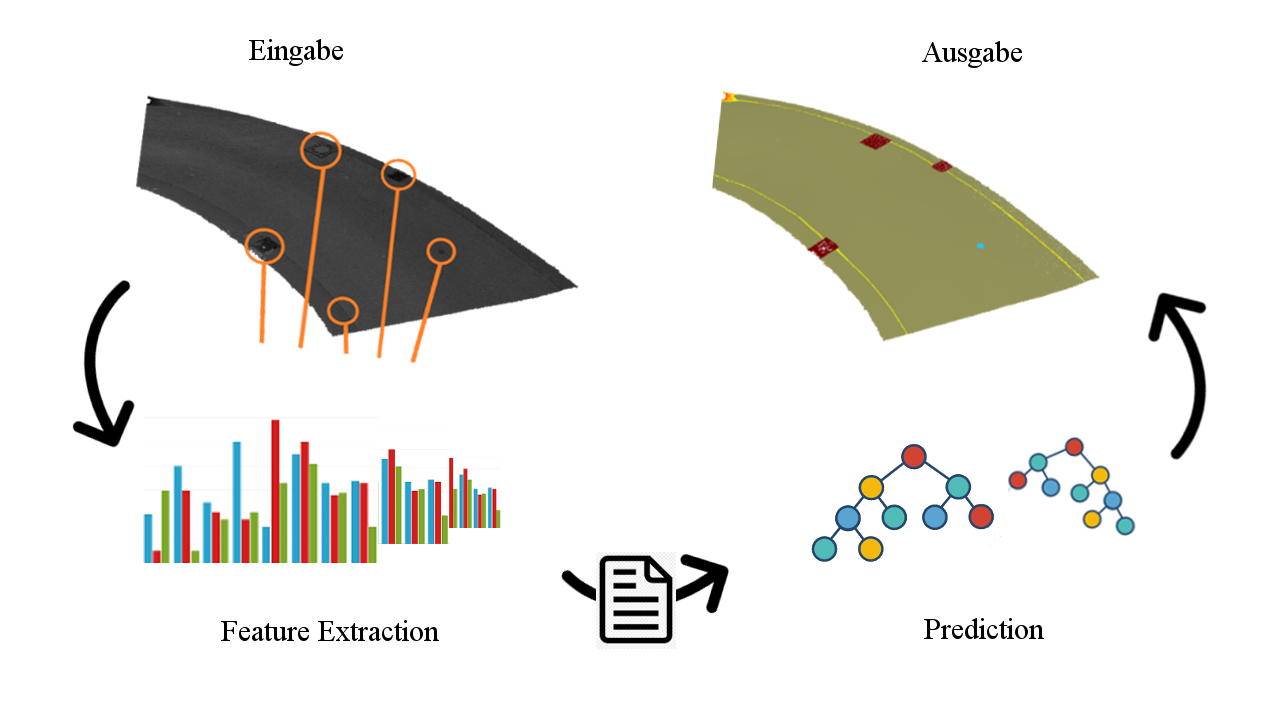
\includegraphics[width=0.95\textwidth]{graphics/ml_process_adv}
    \caption{Ein High-Level-Blick auf den Ablauf des Feature-Extraction-Ansatzes.}
    \label{fig:ml_process}
\end{figure}

\section{Betrachtete Objektklassen}

Entsprechend des Ziels nehmen Objekte, die auf einen mangelhaften Straßenzustand hinweisen, den vornehmlichen Fokus ein. Einfluss auf die Entstehung von Schäden verschiedener Art haben unter anderem der Niederschlag, temperaturbedingte Verformungen sowie die Verkehrsbelastung selbst.\footnote{https://www.ise.kit.edu/rd\_download/SBT/Kolloquium\_SBT\_2011-11-23\_C.Karcher.pdf} Es existieren Leitfäden\footnote{https://itzeb.heller-ig.de/leitfaden/} zur empfohlenen Auswertung solcher \textit{Substanzmerkmale}, an denen sich unter anderem bezüglich der verschiedenen Klassen orientiert wurde. Diese Klassen sind zum besseren Verständnis als Bilder von Punktwolken in Abbildung \ref{fig:all_classes} dargestellt.

\begin{figure}
    \subcaptionbox{unbeschädigte Straße}{
\includegraphics[width=0.32\textwidth]{graphics/class_undamaged}}
    \hfill
    \subcaptionbox{Schlagloch}{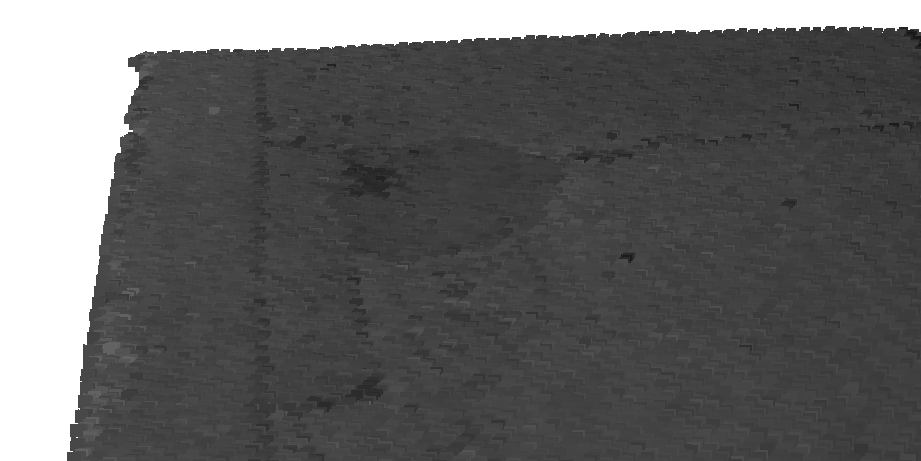
\includegraphics[width=0.32\textwidth]{graphics/class_pothole}}
    \hfill
    \subcaptionbox{Flickstelle}{
\includegraphics[width=0.32\textwidth]{graphics/class_flickstelle}}
    \par\medskip
    \subcaptionbox{Gullys unterschiedlicher Ausprägung}{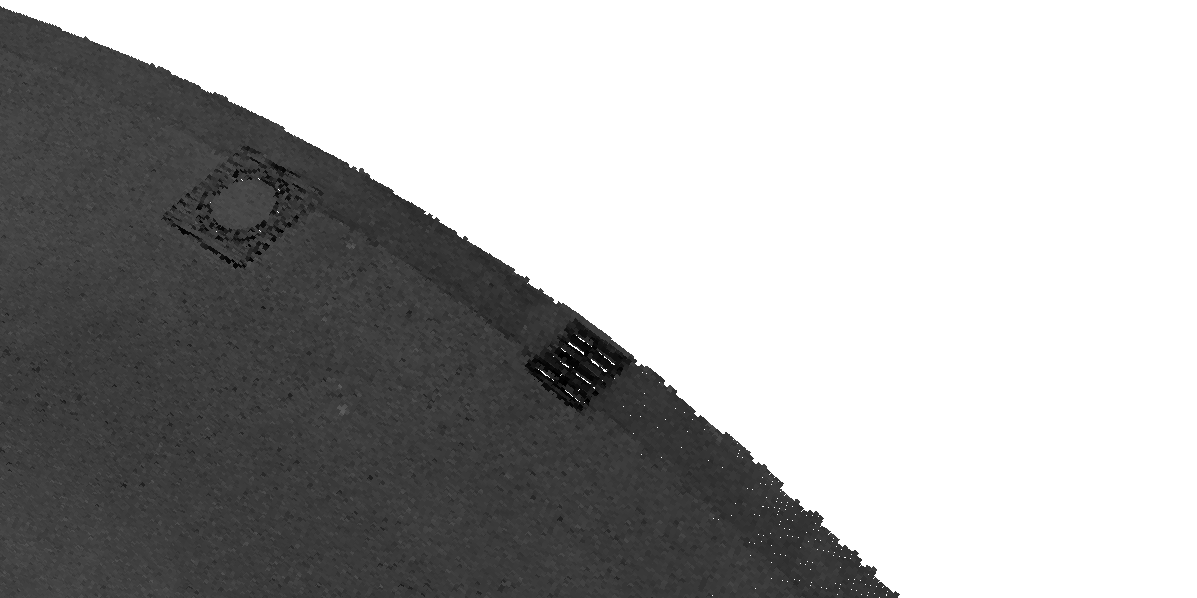
\includegraphics[width=0.32\textwidth]{graphics/class_gully}}
    \hfill
    \subcaptionbox{Ölfleck}{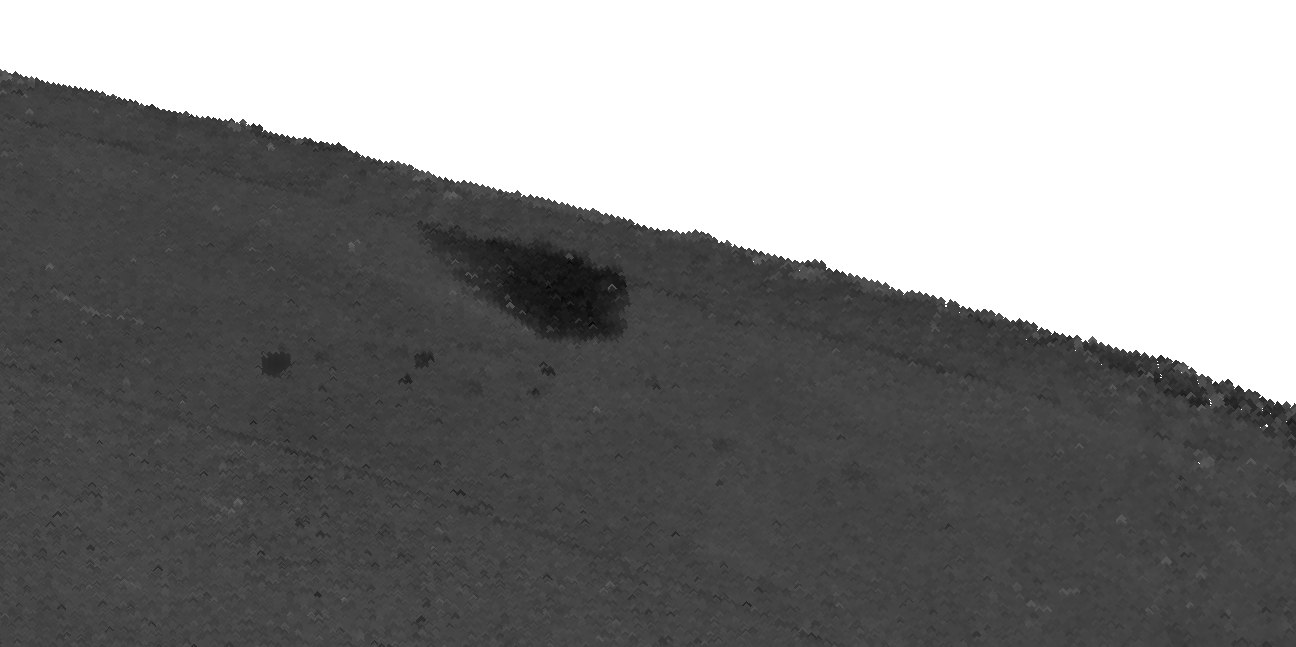
\includegraphics[width=0.32\textwidth]{graphics/class_spill}}
    \hfill
    \subcaptionbox{Fahrbahnmarkierung}{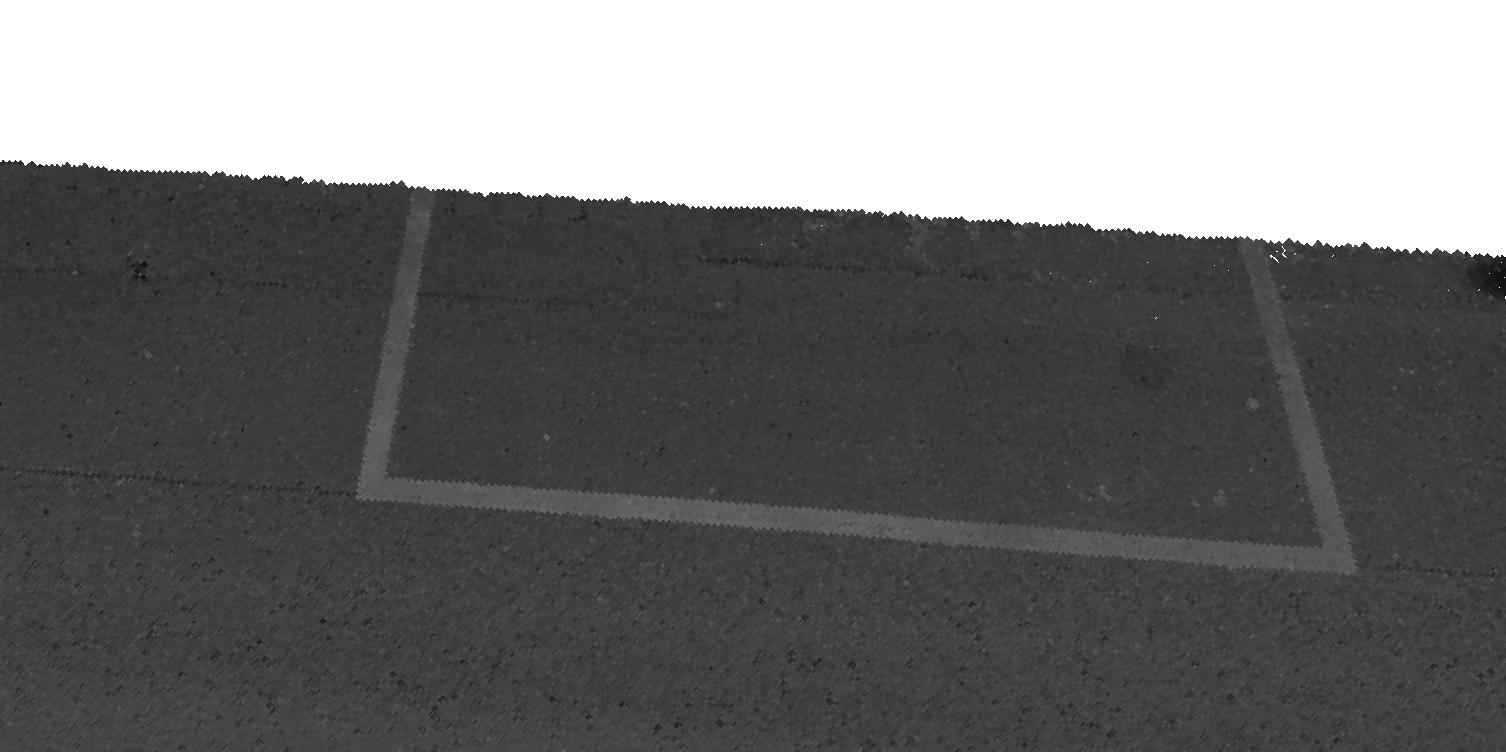
\includegraphics[width=0.32\textwidth]{graphics/class_road_marking}}
    \caption{Beispielhafte Bilder von zu erkennenden Objekten.}
    \label{fig:all_classes}
\end{figure}

Darunter fallen insbesondere merkliche Absenkungen wie Schlaglöcher oder Risse. Schlaglöcher zeichnen sich durch lokale Höhenunterschiede, welche von mehreren Millimetern bis hin zu einigen Zentimetern reichen können, sowie ihre meist eher rundliche Form aus. Durch den Aufriss der Fahrbahnoberfläche erscheinen sie außerdem dunkler als ihre unmittelbare Umgebung. \\
Auch Flickstellen bilden eine - im Vergleich zur gewöhnlichen Straße - auffällige Klasse: Sie werden angebracht, um beschädigte Straßenteile - wie zum Beispiel ein Schlagloch - zu überdecken und auf diese Weise ungefährlich zu machen. Charakterisiert werden sie durch ihre wegen der maschinellen Fertigung meist rechteckige Struktur sowie der im Vergleich zur Nachbarschaft oft dunkler erscheinenden Fugendichtmasse. Letztere kann durch Überquellen ebenfalls für marginale Höhenunterschiede an den Rändern sorgen. Flickstellen werden selbst bei Asphaltbelag auch zu den Schadensklassen gerechnet\footnote{https://itzeb.heller-ig.de/leitfaden/index.html?flickstellen\_\_\_fli\_efli\_afli.htm}. Straßenabschnitte mit einem hohen Anteil an Flickstellen sind entsprechend ein Hinweis auf nötige Reparaturen. \\
Gullys und Kanaldeckel kommen in vielen Ausprägungen bezüglich Größe und Form vor. Obwohl diese selbstverständlich begründet angelegt werden, zeichnen auch sie sich durch charakteristische Höhenunterschiede aus. Diese allgemeine Ähnlichkeit zu Schlaglöchern wirft die Frage nach ihrer Unterscheidbarkeit bezüglich ihrer Features auf, weshalb Gullys ebenfalls ein Ziel der Erkennung sind. Ein zuverlässiges Erkennen von Gullys kann außerdem, wie in Kapitel \ref{chap:uniqueness} erläutert wird, einen weiteren Vorteil bringen: Aufgrund ihrer beständigen Struktur können mehrere Punktwolken desselben Straßenabschnitts zueinander ausgerichtet werden. Damit könnte etwa die Veränderung des Straßenzustands in einem bestimmten Zeitraum dokumentiert werden. \\
Eine weitere Auffälligkeit sind besonders dunkle, unregelmäßige und teils sehr große Flecken. Ohne genaue Betrachtung vor Ort ist nicht zweifelsfrei auszumachen, worum es sich handelt: Bindemittelaustritte sind eine Alternative, aber auch Ölflecken sind möglich und (wegen der Nähe zu Parkplätzen in den genutzten Punktwolken) an dieser Stelle plausibel. Frische Ölflecken allerdings stellen augrund der geringen Griffigkeit eine große Rutschgefahr dar. Wegen dieser Option werden auch jene Stellen gesondert behandelt; der Einfachheit halber ist in der Arbeit folgend nur die Rede von Ölflecken. \\
Für den sicheren Straßenverkehr unerlässlich sind Fahrbahnmarkierungen. Durch ihre in der Materialzusammensetzung begründete Helligkeit sollen sie sich zu allen Tageszeiten und Wetterbedingungen stark abheben vom Rest der Fahrbahn und so Orientierung bieten. Von Interesse könnte hier insbesondere sein, ob und welche Markierungen sich stellenweise durch Verschleiß nicht mehr ihrem Zweck gemäß genug abheben und einer Auffrischung oder Erneuerung bedürfen. \\\\
Für die Bewertung des Straßenzustands spielen auch andere Elemente eine Rolle als unregelmäßige Schäden der Fahrbahnoberfläche wie Schlaglöcher. Dazu zählen zum Beispiel Spurrillen oder Unebenheiten der Straße auf Quer- und Längsseite um wenige Prozent, die unter Umständen über mehrere Meter gemessen werden. Andere Arbeiten wie \cite{Zhiqiang.etal-2019} und \cite{Famili.etal-2021} beziehen diese Mängel als Klassen in ihre \textit{Predictions} ein. \\
Die Erkennung solcher Schäden war kein Ziel dieser Arbeit, entweder aus Mangel an geeigneten und ausreichend vielen Daten oder, da andere Verfahren besser geeignet erscheinen. Für die Berechnung der Quer- wie Längsebenheit kommen beispielsweise 4$m$-Latten\footnote{http://www.vsvinrw.de/tl\_files/VSVI-NRW/Downloads/Seminarberichte/05\_2011/Oberflaecheneigenschaften\_und\_Strassenbautechnik.pdf} zum Einsatz, welche in regelmäßigen Abständen quer zur und längs der Straße gelegt werden. Anhand der Höhendifferenzen der Lattenenden können die gesuchten Werte mathematisch präzise ermittelt werden, ebenso andere Kenngrößen wie die Spurrinnentiefe oder fiktive Wassertiefe. Dieses Prinzip kann übertragen werden auf imaginäre Latten und Punktwolken der Straßen. Famili \textit{et al.} \cite{Famili.etal-2021} verfolgen ähnliche Vorgehensweisen über Funktionsgraphen von Querschnitten der Oberfläche. Solche geometrischen Verfahren sind bereits algorithmisch zu akkuraten Ergebnissen fähig. \\
Erst durch Kombination von Ansätzen, die sich auf solche verschiedenen Aspekte fokussieren, kann letztlich ein gesamtheitliches und aussagekräftiges Bild des Straßenzustands geschaffen werden. 

\section{Systemüberblick}

Beide Ansätze bauen auf ein System von bestehenden und abgeschlossenen Tools auf. Diese wurden teilweise ergänzt um nötige Erweiterungen für den \textit{Feature-Extraction}-Ansatz. \\\\
Das in dieser Arbeit bedeutsamste Werkzeug für die Prozessierung von Punktwolken ist das (in Kapitel \ref{chap:intro} kurz eingeführte) \texttt{PCTool}, einer in \texttt{C++} geschriebenen Anwendung. Dieses Framework bietet eine Vielzahl an Möglichkeiten zur effizienten Verarbeitung von Punktwolken. Die Grundbausteine sind sogenannte Knoten (\textit{Nodes}), die jeweils eine Operation zu Eingabe, Ausgabe oder Prozessierung implementieren. Dazu gehören zum Beispiel \textit{Reader} und \textit{Writer} von Punktwolken verschiedener Dateiformate. Auch die bereits erwähnten Funktionalitäten der Dichtereduktion und Bodenerkennung finden sich dort als separate Knoten wieder neben den für den eigenen Ansatz implementierten. Um die Knoten zu komplexeren Aktionen zu verknüpfen, können sie zu \textit{Pipelines} zusammengelegt werden. Ein Beispiel dazu findet sich in Abbildung \ref{fig:pcr_pipeline}, wo der beschriebene Ablauf des ersten Teils des eigenen Ansatzes zu sehen ist: vom Einlesen der Punktwolke, der Bodenerkennung und Straßenextraktion bis zum Ermitteln der Featurevektoren der einzelnen Punkte zur Schadenserkennung und Zurückschreiben der Punktwolke. (Anmerkung: Der einzelne \texttt{GroundDetector}-Knoten steht an dieser Stelle nur stellvertretend für die im Projekt genutzte elaboriertere Bodenerkennung, siehe \cite{Mattes-2021}.) Auf die Hintergründe der \texttt{StreetExtractor}- und \texttt{PavementDistressDetector}-Knoten wird in nachfolgenden Kapiteln näher eingegangen. \\\\

\begin{figure}[!ht]
    \centering
    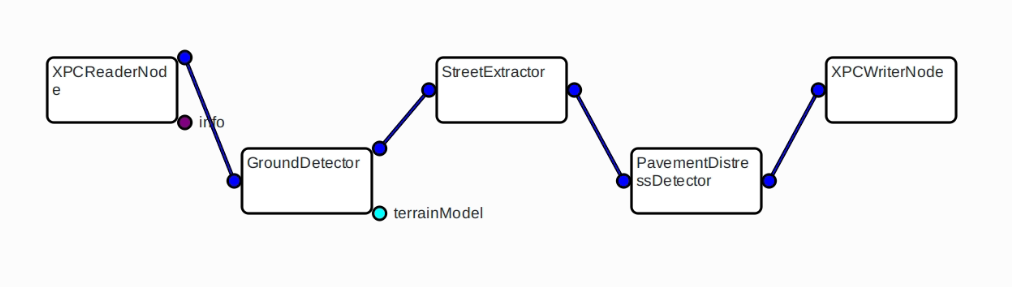
\includegraphics[width=0.95\textwidth]{graphics/pcr_pipeline}
    \caption{Die eingesetzte Pipeline im PCTool für die Featureberechnung.}
    \label{fig:pcr_pipeline}
\end{figure}

Der zweite Schritt des \textit{Feature-Extraction}-Ansatzes, den \textit{Predictions} der einzelnen Punktklassen anhand der Featurevektoren, findet sich in einer Reihe von Python-Skripten. Diese sind Teil des im Projekt entstandenen sogenannten \textit{Modelzoo}, der eine Menge von Funktionalitäten des maschinellen Lernens für die Webplattform \citep{Schilling-2021} bietet. Unter anderem ist dort auch die Klassifizierung von Punktwolken anhand ihres sogenannten \textit{Point Cloud Fingerprints} gelegen, einer Art globaler und kompakter Repräsentation \citep{Kirsten-2021}. Für den eigenen Ansatz werden vor allem Schnittstellen zum Trainieren und Testen von Modellen für die \textit{Predictions} obiger Klassen bereitgestellt, siehe Kaptiel \ref{chap:prediction}. \\
Der Grund für die Trennung der Featureberechnung und \textit{Prediction} in zwei Teilsysteme, was einen verhältnismäßig hohen Zusatzaufwand bedeutet durch Übertragung und Zwischenspeicherung der Featurevektoren, liegt in der Handhabbarkeit. Python ist im Bereich des maschinellen Lernens eine etablierte Wahl und bietet insbesondere einfach zu nutzende Schnittstellen. Langfristig ist daher für eine Effizienzsteigerung die Integration des \textit{Prediction}-Teilsystems in \texttt{C++} bzw. im Speziellen das \texttt{PCTool} anzustreben. \\\\
Mit Hilfe des \texttt{PCNN}-Frameworks, in Kapitel \ref{chap:intro} eingeführt, wurde der \textit{Deep-Learning}-Ansatz getestet. Näheres zur Architektur und Bedienung findet sich in Kapitel \ref{chap:deepl}. Etwaige Bilder von Punktwolken wurden angefertigt mit dem lehrstuhleigenen \texttt{PCViewer}, welcher eine Vielzahl an Möglichkeiten zur Visualisierung der einzelnen Punkte bietet. \\
Das letzte im Zuge dieser Arbeit genutzte Programm ist das \texttt{TrainingTool}, das der Annotation der Klassen pro Punkt dient. Um sich eine Grundlage für die Experimente dieser Arbeit zu schaffen und mangels geeigneter vorhandener Datensätze, wurden damit die Schlaglöcher, Gullys und alle weiteren erwähnten Klassen manuell nach bestem Wissen und Gewissen markiert. Insbesondere wegen der teils feinen Objekte sowie der begrenzten Auflösung der Punktwolken ist damit aber immer eine Unsicherheit behaftet. Gerade bezüglich der Grenzen von Flickstellen und Ränder von Schlaglöchern ist diese Einschränkung in der qualitativen und quantitativen Analyse der \textit{Predictions} zu berücksichtigen, die sich in Kapitel \ref{chap:eval} findet.
%!TEX root = foo-thesis.tex

\chapter{Preprocessing}
\label{chap:preproc}

Die Berechnung der Featurevektoren zur Schadenserkennung wird nicht unmittelbar auf der eingehenden Punktwolke ausgeführt, sondern bedarf zunächst einer Vorprozessierung. \\
Die erste Aufgabe besteht darin, den Boden der Punktwolke zu bestimmen und damit die Menge der für diesen Anwendungsfall überhaupt bedeutsamen Punkte zu reduzieren. Dazu wird eine Bodenerkennung (\textit{Ground Detection}) eingesetzt, welche unter anderem mit Höhenmodellen arbeitet und im Projekt auf der im \texttt{PCTool} bereits bestehenden Funktionalität aufbaut. Schließlich werden die als Boden erkannten Punkte mit der entsprechenden semantischen Klasse markiert. Der nachfolgende Schritt beruht auf einem guten Ergebnis der Bodenerkennung in dem Sinne, dass möglichst viele Punkte der Straße erhalten bleiben und restliche Punkte nicht die Bodenklasse zugewiesen bekommen. Auf die Hintergründe und Implementierung der ausgereifteren Bodenerkennung wird hier nicht näher eingegangen, dies ist bei \cite{Mattes-2021} zu finden.

\section{Straßenextraktion}

Mit den Informationen zum Boden folgt der Schritt, der die Straße selbst erkennen soll. Diese Straßenextraktion soll also außenstehenden Rasen, niedrige Häuserwände und sonstige als Boden klassifizierte, aber nicht zur Fahrbahn selbst gehörenden Bereiche entfernen. Die Grundlage dafür ist eine Abschätzung der Trajektorie des \textit{Mobile-Mapping}-Fahrzeugs, also dessen gefahrener Strecke, die ja auf der Straße verläuft. Diese Abschätzung beruht auf den Dichten der einzelnen Punkte, das bedeutet wie viele Nachbarn sie in einem gewissen Radius besitzen. Bedingt durch die Arbeitsweise der Laserscanner werden nämlich nahegelegene Oberflächen deutlich dichter abgetastet als weiter entfernte \citep{Li.etal-2019}. Wegen der Montierung des Laserscanners auf dem Fahrzeug sind die Punkte auf der gefahrenen Strecke entsprechend dichter als etwa die andere Straßenseite und sonstige Oberflächen. Eine Visualisierung dessen findet sich in Abbildung \ref{fig:colored_density}. \\

\begin{figure}
    \subcaptionbox{Die Straße eingefärbt nach dem Intensitätswert.}{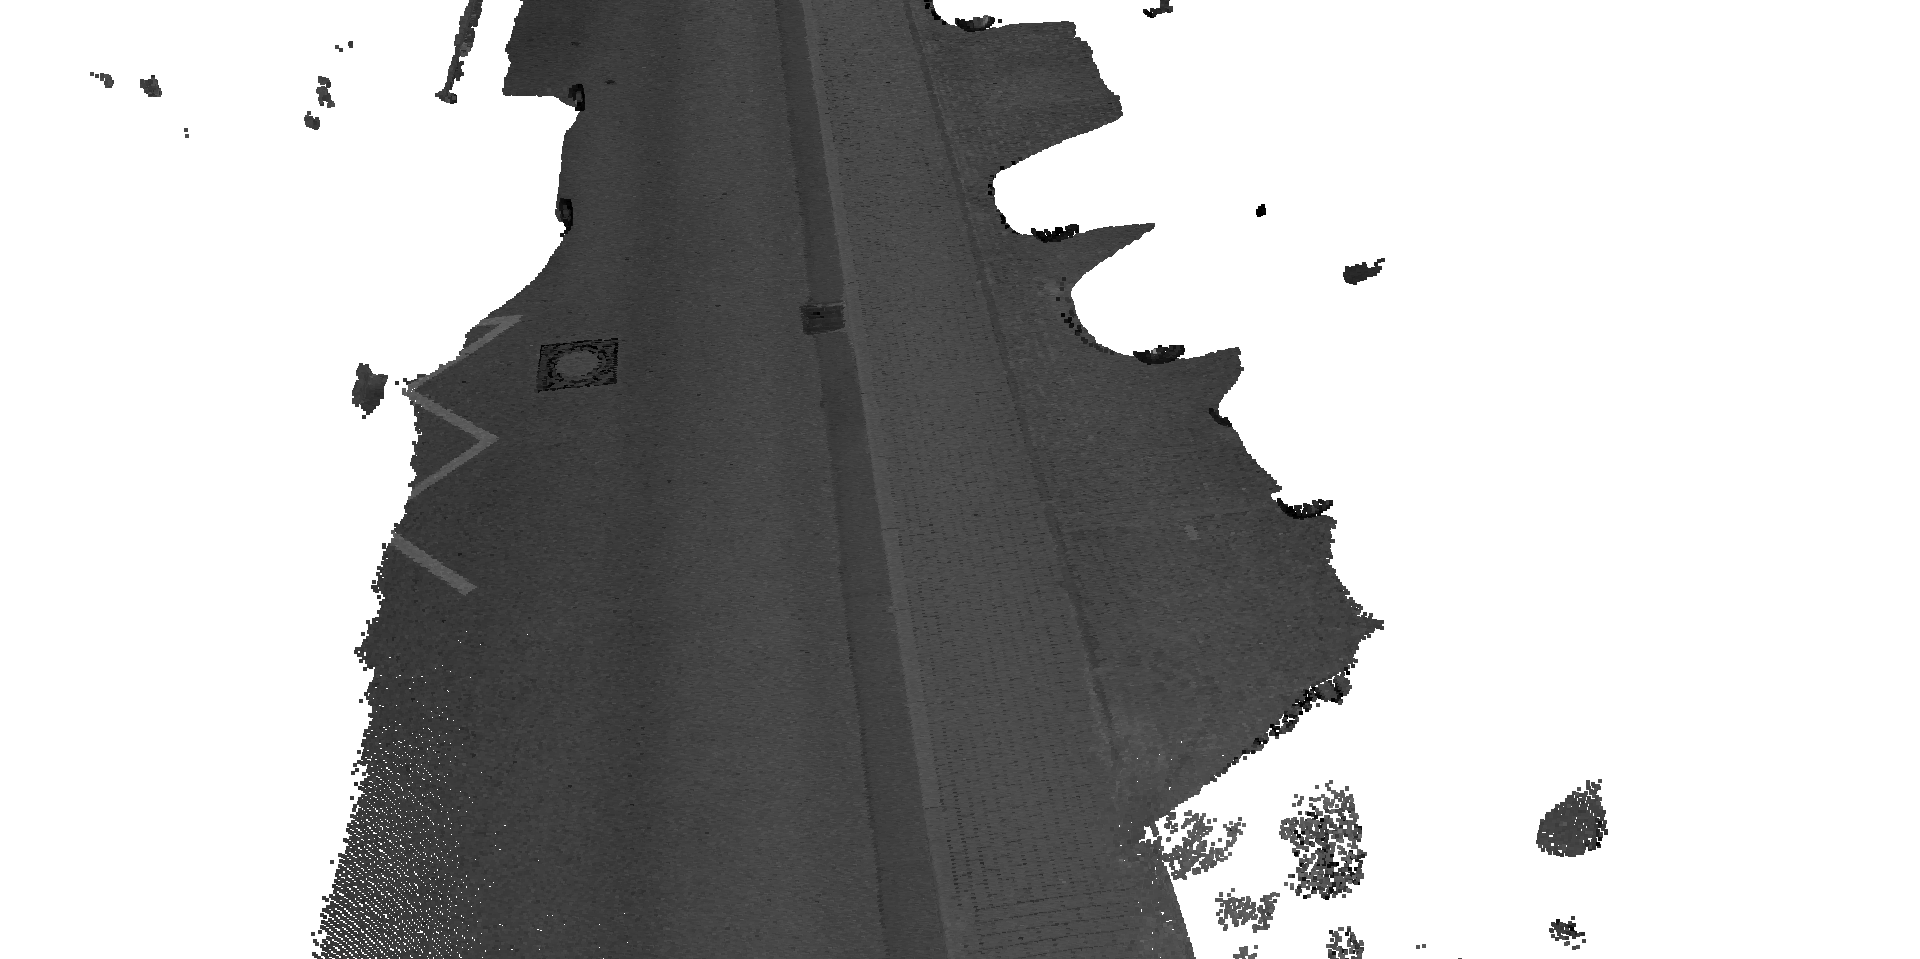
\includegraphics[width=0.5\textwidth]{graphics/trajectory_intensity}}
    \hfill
    \subcaptionbox{Die Straße eingefärbt nach ihren Punktdichten.}{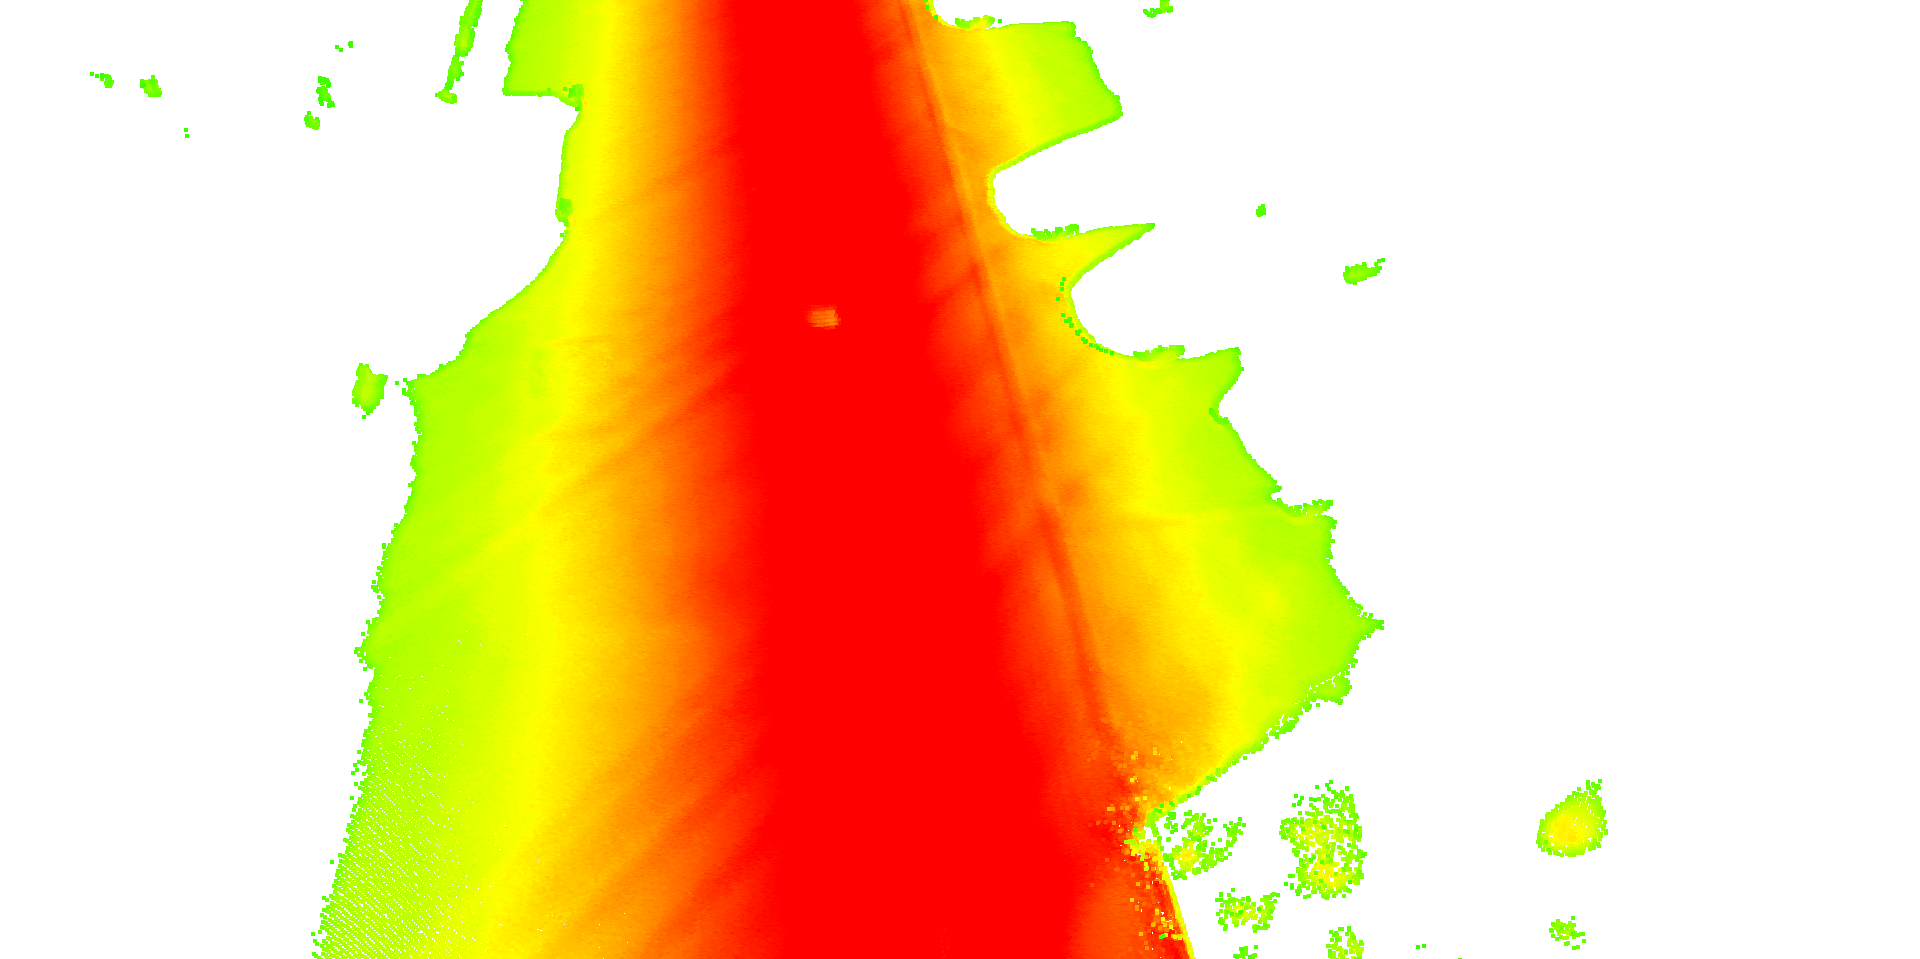
\includegraphics[width=0.5\textwidth]{graphics/trajectory_colored}}
    \caption{Eingefärbte Dichten der Punktwolke nach stattgefundener Bodenerkennung und Entfernung des Nicht-Bodens. Je roter der Farbton eines Punktes, umso dichter ist dessen Umgebung. Die abgeschätzte Trajektorie umfasst eine Straßenseite sowie den Gehweg auf dieser Seite.}
    \label{fig:colored_density}
\end{figure}

Da sich die konkreten Dichten je nach genutztem Laserscanner und somit pro Punktwolke unterscheiden können, werden die gesammelten Dichten zu relativen Werten umgewandelt. Dabei kommt die sogenannte \textit{Min-Max}-Normalisierung zum Einsatz \citep{Patro.Sahu-2015}. Das bedeutet, von jedem einzelnen Wert der Liste - hier der Dichten pro Punkt - wird das Minimum der Liste subtrahiert und anschließend durch die Differenz von Maximum und Minimum geteilt. Auf diese Weise ist in der verarbeiteten Liste immer der kleinste Wert die 0 und der größte Wert die 1. Diese nun relativen Dichten sind über verschiedene Punktwolken hinweg besser vergleichbar. \\\\
Mit Hilfe des arithmetischen Mittels und der Standardabweichung der relativen Dichten wird die Punktwolke in zwei Teile getrennt: Der erste Teil repräsentiert die abgeschätzte Trajektorie, die zumindest größtenteils zur Straße dazugehören soll. Der zweite Teil beinhaltet die restlichen Punkte, wozu die andere Straßenseite und sonstige übrig gebliebene Oberflächen zählen können, die also teilweise auch als Straße erkannt werden sollen. Dabei zählen all jene Punkte, deren relative Dichte größer als das arithmetische Mittel minus einer halben Standardabweichung ist, zum Trajektorie-Teil. Der Faktor wurde empirisch bestimmt. \\
Auf den beiden Teilen wird nun parallel der \texttt{PointCloudClusterer} eingesetzt, der bereits im \texttt{PCTool} integriert ist: Dieser ermittelt auf Punktdistanzen basierende zusammenhängende Bereiche, die \textit{Cluster}. Spezifiziert werden kann die maximale Distanz eines Punktes zur Noch-Zugehörigkeit zu einem \textit{Cluster} sowie die minimale Größe eines \textit{Clusters} gegen sein Verwerfen. 
Die maximale Distanz wurde hier auf 20\% der durchschnittlichen relativen Dichte gesetzt, was bei den getesteten Punktwolken einen guten Ausgleich zwischen Straßenbeibehaltung und Entfernung restlicher Punkte bedeutete. Die nötige Größe der \textit{Cluster} beträgt 30\% der Größe der jeweiligen Teilpunktwolke. Dies beruht auf der Annahme, dass in beiden Teilen die Straße den jeweils größten Anteil der Punkte ausmacht, da sie durchgängig verläuft im Gegensatz zu Rasenflächen einzelner Gebäude oder sonstigen nahegelegenen Bodenstellen. Andererseits wird nicht zwangsläufig nur das größte \textit{Cluster} behalten, da es Fälle geben kann, in denen die Straße getrennt voneinander ist - etwa durch parkende Autos, die durch die vorherige Bodenerkennung entfernt worden sind. Diese 30\% sollen also erneut einen Ausgleich herstellen zwischen einer vollständigen Straßenerfassung und möglichst großen Entfernung sonstiger Punkte. All jene \textit{Cluster}, die bis dahin übrig geblieben sind - im Trajektorie-Teil wie im restlichen Teil - werden zur Straße gezählt und zum Schluss wieder zu einer einzelnen Punktwolke zusammengeführt mit dem integrierten \texttt{PointCloudMerger}. Eine geordnete Darstellung dieses Prozesses findet sich in Abbildung \ref{fig:street_extraction}.

\begin{figure}[!ht]
    \centering
    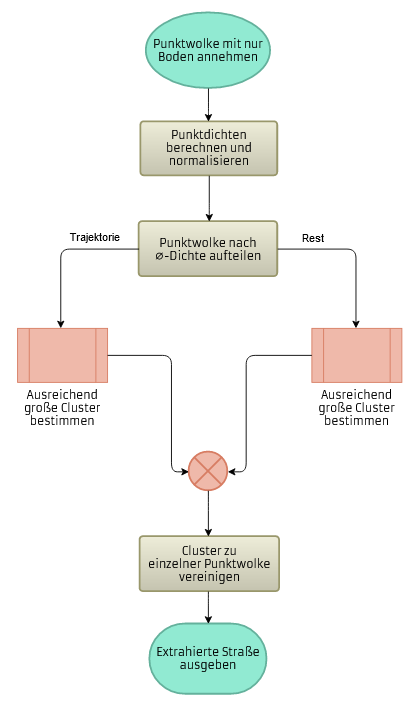
\includegraphics[width=0.5\textwidth]{graphics/flowchart_street_extraction}
    \caption{Eine Übersicht des Ablaufs der Straßenextraktion. Die roten Kästen kennzeichnen die bezüglich Laufzeit aufwändigsten Schritte des Prozesses.}
    \label{fig:street_extraction}
\end{figure}

Dieser Teil der gesamten \textit{Pipeline} sollte keinen Fokus der Arbeit einnehmen, sondern war zunächst rein funktional angelegt und beruht auf einigen Heuristiken. Wie in Kapitel \ref{chap:eval} dargestellt wird, reicht dies bereits aus für den Erhalt der fast vollständigen Straße und großer Reduktion sonstiger Punkte. Nachteilig ist, dass der Prozess Parameter beinhaltet, die bisher nur nach reinem Empfinden und an wenigen Testpunktwolken bestimmt wurden. Für denkbare Verbesserungen der Straßenextraktion neben diesem Ansatz siehe Kapitel \ref{chap:outro}. \\
Sobald die nun als Straße erkannten Punkte extrahiert sind, dient die nun übrige Punktwolke beiden Ansätzen als Eingabe ihrer Verarbeitung.

\section{Normalisierung der Intensität}

Vor der tatsächlichen Berechnung der Features erfolgt noch eine Wertenormalisierung. Während der \textit{Deep-Learning}-Ansatz seine eigene Art der Normalisierung vornimmt, geht der eigene Ansatz folgendermaßen vor: 
Oftmals wird neben den 3D-Koordinaten der Punkte auch ihre Intensität erfasst und gespeichert, ein Maß zur Ermittlung der Stärke des reflektierten Laserstrahls \citep{Tatoglu.Pochiraju-2012}. Dieses Intensitätsattribut besitzt eine hohe Varianz bezüglich verschiedener Laserscanner, die unter anderem von deren unterschiedlicher Technik oder Verarbeitung verursacht wird. Zwar liegt der Wertebereich des Attributs grundsätzlich bei 0 bis 65535, wird aber meist nicht ausgenutzt. Der Intensitätswert desselben Punktes, aufgenommen von zwei verschiedenen Laserscannern, kann sich um mehrere Tausend unterscheiden. Aus diesem Grund werden diese absoluten Werte zunächst in relative umgewandelt, sodass sie über verschiedene Punktwolken hinweg vergleichbar sind. Für die Normalisierung wird ebenfalls die \textit{Min-Max}-Normalisierung verwendet, wie sie im vorigen Abschnitt erläutert wurde. Dadurch hat letztlich die geringste Intensität der Punktwolke den Wert 0 und die höchste den Wert 1. Eine ähnliche Normalisierung und Anpassung des Wertebereichs findet sich bei \cite{Li.Cheng-2018}. Ein Nachteil dessen ist der Verlust der absoluten Dimension der Intensität. Dies könnte zum Beispiel dann problematisch sein, wenn eine Punktwolke keine Fahrbahnmarkierungen beinhaltet, die für gewöhnlich die hellsten Objekte auf der Straße sind. In diesem Fall würden durch die Normalisierung Punkte einer anderen Klasse die höchsten Werte nahe der 1 erhalten, was sich unter Umständen negativ auf die auf diesem Feature aufbauenden \textit{Predictions} auswirkt. \\
Da bei den 3D-Koordinaten keine so erheblichen Unterschiede zu erwarten sind, werden diese Werte nicht normalisiert und alle letztlich daraus ermittelten Features als vergleichbar über verschiedene Punktwolken hinweg angesehen. \\\\
Ein weiterer Aspekt, der eine schädliche Wirkung auf die Qualität der \textit{Predictions} haben kann, sind einzelne Punkte, deren Intensität übermäßig stark von der Mehrheit der anderen Werte abweicht. Unabhängig davon, ob dies Messungenauigkeiten sind oder tatsächlich einzelne Abweichungen, wird diese Anomalie in die Normalisierung übernommen und daher ist ein Entfernen jener Werte erstrebenswert. Da aber selbstverständlich auch diese Punkte erhalten bleiben und eine Intensität besitzen sollen, werden die Außenseiter-Punkte noch vor der Normalisierung bestimmt und ihre Intensität auf den niedrigsten bzw. höchsten Wert gesetzt, der nicht zu den abweichenden Werten gezählt wird. Auf diese Weise sollen die Relationen zwischen verschiedenen Punktwolken annähernd erhalten bleiben, ohne durch die Werteanpassung und anschließende Normalisierung einen merklichen Informationsverlust zu erleiden. \\
Der hier genutzte Prozess zum Finden abweichender Punkte basiert auf der \textit{Interquartile Range (IQR)} \citep{Rousseeuw.Hubert-2011}. Dabei werden die Werte an einem Viertel sowie drei Viertel (zur Ganzzahl abgerundet bzw. aufgerundet) der sortierten Liste angeschaut: Dies sind das erste bzw. dritte Quartil $Q_1, Q_3$. Mittels $IQR = Q_3 - Q_1$ können nun die angesprochenen Schwellwerte nach oben und nach unten definiert werden als
\begin{equation}
    T_{lo} = Q_1 - s * IQR  
        \quad\text{und}\quad 
    T_{hi} = Q_3 + t * IQR
\end{equation}
Alle Werte kleiner als $T_{lo}$ werden schließlich auf $T_{lo}$ gesetzt; alle Werte größer als $T_{hi}$ werden auf $T_{hi}$ gesetzt. Die einzigen Parameter, die dafür noch festgelegt werden müssen, sind $s$ und $t$. Sie bestimmen, wie schnell ein Wert als Außenseiter betrachtet wird. Häufig liegen um $1,5$, in diesem Fall werden sie - auch bedingt durch die große Spannbreite des Wertebereichs mit starker Konzentration in der Mitte wegen der gewöhnlichen Straßenpunkte - empirisch mit $s=6$ bzw. $t=4$ belegt. Konkrete Zahlen zu den Auswirkungen auf Trainings- und Testpunktwolke finden sich in Kapitel \ref{chap:eval}.
%!TEX root = foo-thesis.tex

\chapter{Featureberechnung}
\label{chap:feature-calc}

Im Folgenden sollen die wichtigsten Bestandteile der Featureberechnung im \textit{Feature-Extraction}-Ansatz motiviert und erläutert werden. Der vollständige Ablauf des Prozesses, der noch das im nächsten Kapitel behandelte \textit{Uniqueness}-Konzept beinhaltet, findet sich dort in Abbildung \ref{fig:feature_extraction}. Die Featureberechnung ermittelt letztlich für jeden Punkt dessen Featurevektor, der vom Modell zur \textit{Prediction} der Klasse genutzt wird.

\section{Scales}

Um einen Punkt zu charakterisieren, wird seine lokale Nachbarschaft betrachtet. Für die Ermittlung dieser Nachbarschaft gibt es zwei häufig genutzte Wege: die \textit{k} nächsten Nachbarn zu nehmen oder alle Nachbarn, die im vorgegebenen Radius einer Kugel um den Ursprungspunkt liegen. Der Vorteil an den \textit{k} Nachbarn ist, dass man sich über die betrachtete Nachbarzahl sicher sein kann. Allerdings hängt der dabei betrachtete Radius erheblich von der lokalen Punktdichte ab: Beim \textit{Mobile Mapping} etwa wird für Punkte auf der Trajektorie des Laserscannerfahrzeugs mit demselben \textit{k} ein deutlich geringerer Radius betrachtet als für Punkte auf der anderen, nicht befahrenen Straßenseite. Abbildung \ref{fig:knn_vs_scale} stellt dies an zwei Beispielpunkten anschaulich dar. Deshalb eignet sich die Radiusbetrachtung besser für konsistente und über verschiedene Punkte vergleichbare geometrische Features \citep{Thomas.etal-2018}. Diese Art der Nachbarschaftsbetrachtung - von nun an werden die Radii \textit{Scales} genannt - findet in dem \textit{Feature-Extraction}-Ansatz entsprechend Verwendung. \\

\begin{figure}
    \subcaptionbox{Trajektorie, k = 60}{
\includegraphics[width=0.5\textwidth]{graphics/traj_knn_adv}}
    \hfill
    \subcaptionbox{Nicht-Trajektorie, k = 60}{
\includegraphics[width=0.5\textwidth]{graphics/nontraj_knn_adv}}
    \par\medskip
    \subcaptionbox{Trajektorie, Radius 10cm}{
\includegraphics[width=0.5\textwidth]{graphics/traj_scale_adv}}
    \hfill
    \subcaptionbox{Nicht-Trajektorie, Radius 10cm}{
\includegraphics[width=0.5\textwidth]{graphics/nontraj_scale_adv}}
    \caption{Visualisierungen der Nachbarschaften zweier Punkte (zentral, rot gefärbt) auf der Trajektorie bzw. dem restlichen Teil, ermittelt durch die k nächsten Nachbarn bzw. einen festen Radius. Die Bilder sind maßstabsgerecht.}
    \label{fig:knn_vs_scale}
\end{figure}

Um trotz der oftmals Millionen von Punkten einer Punktwolke schnell positionelle Beziehungen herzustellen, wozu etwa das Finden der Nachbarschaft eines Punktes gehört, bedarf es dafür geeigneter Datenstrukturen. Eine solche ist auch der \textit{k-d}-Baum, der einen effizienten Zugriff auf multidimensionale Daten erlaubt, wie es die 3D-Punktkoordinaten sind. Das \texttt{PCTool} sieht dafür die Klasse \texttt{SpatialSearch} vor, die intern einen \textit{k-d}-Baum implementiert und eine einfach zu nutzende Schnittstelle bietet. So können mit jeweils einem Funktionsaufruf sowohl die \textit{k} nächsten Nachbarn einer 3D-Position oder eines Punktindizes gefunden werden als auch alle Nachbarn in einem vorgegebenen Scale. \\\\
Die nächste Frage ist, welche konkreten Scales genutzt werden. Dass überhaupt die Nutzung mehrerer Scales sinnvoll ist, zeigt sich beim Blick auf verschiedene Objekte, die es zu erkennen gilt. Zum einen sind gerade Schlaglöcher häufig unregelmäßige Strukturen, die in vielerlei Ausprägungen vorkommen können: über mehrere Größen hinweg sowie in sehr runden oder eher länglichen Formen. Flickstellen zeichnen sich vorzugsweise in kleinem Scale aus durch ihre hohen Intensitätsunterschiede zu ihrer Umgebung. Bei größeren Gullys wird der innere, mittige Bereich hingegen erst mit deutlich größerem Scale auffällig, da er im kleinen Bereich sehr planar und kaum von der gewöhnlichen Straße zu unterscheiden ist. Um mit diesen verschiedenen Granularitäten umgehen zu können, werden mehrere, an typische Objektgrößen angepasste, Scales genutzt. \\
Um einen Eindruck von den durchschnittlichen Nachbarzahlen verschiedener Scales zu erhalten, sind diese in Tabelle \ref{table:neighbor_counts} (auf Ganzzahlen gerundet) aufgelistet für die Trainingspunktwolke, jeweils auch separat für den Trajektorie- und den restlichen Teil. Den Daten ist Folgendes zu entnehmen:
\begin{itemize}
    \item Für größere Scales steigen die Nachbarzahlen immer stärker an.
    \item Die Nachbarzahlen für Punkte auf der abgeschätzten Trajektorie sind in etwa doppelt so hoch wie für Punkte auf der restlichen Punktwolke. Dies gibt eine weitere Begründung für die in der Straßenextraktion vorgenommene Trennung in einen Trajektorie- und einen restlichen Teil.
    \item Die gesamtheitlichen Zahlen eines Scales liegen näher an denen der Trajektorie. Dies verdeutlicht die Tatsache, dass auf der vom Laserscannerfahrzeug gefahrenen Strecke deutlich mehr Punkte erfasst werden als in der übrigen Umgebung.
\end{itemize}
Laufzeiten für insbesondere die größeren Scales werden in Kapitel \ref{chap:eval} aufgeführt, doch wird hieraus bereits die Beschränkung auf möglichst kleine Scales ersichtlich.

\begin{table}
\centering
\begin{tabular}{c|c|c|c|c|c|c|c|c|c|c}
 & 1$cm$ & 3$cm$ & 6$cm$ & 9$cm$ & 12$cm$ & 15$cm$ & 20$cm$ & 30$cm$ & 40$cm$ & 50$cm$ \\
\hline
Trajektorie & 2 & 15 & 58 & 131 & 232 & 361 & 639 & 1417 & 2480 & 3812 \\
Rest        & 1 &  7 & 28 &  62 & 110 & 171 & 304 &  683 & 1211 & 1887 \\
\hline
\textbf{Gesamt} & \textbf{2} & \textbf{13} & \textbf{48} & \textbf{109} & \textbf{192} & \textbf{299} & \textbf{530} & \textbf{1178} & \textbf{2068} & \textbf{3186} \\
\end{tabular}
\caption{Die durchschnittlichen Nachbarzahlen für ausgewählte Scales, außerdem getrennt aufgeführt für verschiedene Teile der Punktwolke.}
\label{table:neighbor_counts}
\end{table}

Für die unteren Scales wird hier die Grenze bei 3$cm$ angesetzt. Dies ist gering genug für die Feinheiten der Flickstellen oder potenziell sehr kleine Schlaglöcher. Um aussagekräfige Features aus Nachbarschaften zu extrahieren und nicht zu stark von Messungenauigkeiten beeinflusst zu werden, benötigt es eine gewisse Grundanzahl an Nachbarn. Die noch kleineren Scales erfüllen dies - wie der Tabelle zu entnehmen - nicht und werden daher nicht verwendet. Bei den größeren Scales muss abgewogen werden zwischen ihrem zusätzlichen Informationsgehalt und der steigenden Verarbeitungsdauer. Wie bereits erwähnt, sind die großen Scales vor allem sinnvoll für die mittigen Punkte von Gullys. Allerdings genügt auch für diese Punkte ein Scale von etwa 25$cm$, um zu charakteristischen Stellen des Gullys zu reichen wie dem Innenring, weshalb dies die naheliegende obere Schranke darstellt. Da diese Arbeit einen stärkeren Fokus auf die Schadenserkennung legt als auf die vollständige Identifikation von Gullys, liegt der maximale Scale für die standardmäßigen Versuche bei nur 15$cm$. In Kapitel \ref{chap:eval} findet sich auch ein Vergleich zu einem Experiment mit zusätzlichen größeren Scales. In der Spanne von 3$cm$ bis 15$cm$ wird nun jeder Scale im Abstand von wiederum 3$cm$ für die Featureberechnung genutzt. Dies soll einerseits eine angemessene Menge von Scales darstellen, andererseits typische Größen von anzufindenden Schlaglöchern abdecken.

\section{Ein- und mehrwertige Features}

Als Features für Punkte kommen zum einen einwertige Daten in Betracht. Dies umfasst zum Beispiel
\begin{itemize}
    \item Attribute direkt wie die Intensität
    \item Werte, die sich aus der Punktenachbarschaft ergeben, etwa aus der Verteilung der umliegenden 3D-Koordinaten
    \item kumulierte Formen obiger Daten, etwa Durchschnitte oder Standardabweichungen davon
\end{itemize}
Daneben gibt es auch die Möglichkeit für mehrwertige Features. Diese können etwa als Histogramme ausgedrückt werden, also Häufigkeitsverteilungen für bestimmte numerische Merkmale. Sie sind zusammengesetzt aus mehreren sogenannten Bins, welche die Anzahl der Observationen zählen, die in den von ihnen aufgespannten Wertebereich fallen. In dieser Arbeit entspricht eine Observation dem Merkmal eines Punktes, etwa einem Intensitätswert. Die absolute Zahl an Observationen in einem Bin wird \textit{Count} genannt, der entsprechende relative Wert - bezogen auf die Gesamtzahl an Observationen im Histogramm - \textit{Frequency}. Vorteile von Histogrammen sind insbesondere folgende \citep{Rusu.etal-2008}:
\begin{itemize}
    \item Sie besitzen eine grundsätzlich höhere Aussagekraft durch die genauere Charakterisierung der Nachbarschaft. Was sich etwa in einem Durchschnittswert durch entgegengesetzte Größen aufheben würde, kann nun präziser dargestellt werden. Mehr und damit feinere Bins, d.h. jeweils kleinere Wertebereiche, können die Aussagekraft potenziell steigern. Allerdings resultiert dies unter Umständen in einer zu starken Verteilung der Häufigkeiten, sodass charakteristische Ausschläge verloren gehen.
    \item Die oben aufgeführten teilweise erheblichen Unterschiede der Dichte an verschiedenen Stellen einer \textit{Mobile-Mapping}-Punktwolke machen einwertige Features unter Umständen schwierig vergleichbar für einen festen Scale. Bei Histogrammen kann dieses Problem abgeschwächt werden, da durch das Einsortieren in Bins die Werte normalisiert werden in den Bereich von 0 bis 1, und zwar unabhängig von der Anzahl der Nachbarn. Deswegen werden im Ansatz zum Vergleich zwischen Histogrammen und auch für die letztlichen Featurevektoren lediglich die \textit{Frequencies} betrachtet.
    \item Der Umgang mit Außenseiterpunkten (\textit{Outliern}), die teilweise von Messungenauigkeiten stammen, wird erleichtert. Während sie bei einwertigen Features den Wert stark verzerren können - sofern nicht laufzeitintensivere Berechnungen wie der Median durchgeführt werden -, erhöhen sie beim Histogramm nur die \textit{Frequency} eines Bins leicht und sind somit beinahe wie leere Bins zu behandeln. Zwar werden solche \textit{Outlier} bei den Intensitäten im \textit{Preprocessing} möglichst beseitigt. Bei den unnormalisierten 3D-Koordinaten sind sie aber weiterhin möglich und potenziell hinderlich.
    \item Histogramme sind, im Gegensatz zu einigen anderen lokalen Deskriptoren \citep{Han.etal-2018}, unabhängig von Transformationen der Punktwolke wie Rotation oder Translation.
\end{itemize}
Für diesen Ansatz sollen lediglich mehrwertige Features eingesetzt werden. Ein Vergleich mit der Nutzung nur einwertiger Features findet sich in Kapitel \ref{chap:eval}.
Im Zuge dieser Arbeit wurde im \texttt{PCTool} eine eigene Histogramm-Datenstruktur implementiert. Das geschah zum einen aus Mangel an Alternativen, zum anderen, um für den \textit{Feature-Extraction}-Ansatz nötige Methoden wie ein Distanzmaß oder die Berechnung einer durchschnittlichen Repräsentation (siehe Kapitel \ref{chap:uniqueness}) direkt einzubauen. Ansonsten werden gewöhnliche Funktionalitäten bereitgestellt wie das Füllen der Bins mit gegebenen Daten sowie die Rückgabe der ermittelten \textit{Frequencies}. \\
Zum Zwecke der Erweiterbarkeit und optimierter Speichernutzung ist \texttt{Histogram} eine abstrakte Klasse, die nur die Counts speichert. Ein Histogramm kann linear oder nicht-linear sein, je nachdem, ob dessen Bins einen kontinuierlichen und gleichmäßig aufgeteilten Wertebereich aufspannen. Diese Arten werden in den beiden Unterklassen \texttt{LinearHistogram} und \texttt{NonLinearHistogram} umgesetzt mit ihren entsprechenden internen Arbeitsweisen. In diesem Ansatz wurden keine nicht-linearen Histogramme genutzt, was insbesondere an ihrer verhältnismäßig aufwändigen Berechnung liegt: Statt die Bins direkt in einer Iteration der Daten zu befüllen, ist eine vorherige Sortierung letzterer nötig. In Verbindung mit größeren Scales macht sich diese $nlogn$-Komplexität in der Laufzeit bemerkbar. Ein Vorteil der Nutzung nicht-linearer Histogramme könnte aber darin liegen, genauere Kontrolle über die Wertebereiche zu haben, wenn etwa bekannt ist, dass in bestimmten Größenordnungen keine Werte zu erwarten sind. \\ 
Die dritte Unterklasse ist das \texttt{AbsoluteHistogram}. Dieses speichert mehrere (grundsätzlich unabhängige) einwertige Features anstatt echter Bins, die als die \textit{Frequencies} betrachtet werden. Da also keine \textit{Counts} existieren, handelt es sich der grundlegenden Bedeutung nach um kein Histogramm. Die \textit{Frequencies} ergeben summiert auch nicht 1, wobei die im Experiment genutzten einwertigen Features jeweils zwischen 0 und 1 liegen. Es ist vornehmlich eingeführt worden für den einheitlichen Umgang mit ein- und mehrwertigen Features bezüglich der Speicherung und des Distanzmaßes, obwohl die Semantik eine andere ist. \\\\
Wenn in Abschnitten des Wertebereichs kaum Werte tatsächlich vorkommen, hat dies bei linearen Histogramme teilweise viele leere Bins zur Folge, d.h. Bins mit einem \textit{Count} und demzufolge einer \textit{Frequency} von 0. Um während der Featureberechnung und der Zwischenspeicherung aller Featurevektoren etwas Speicher zu sparen, werden solche Folgen von leeren Bins verkürzt abgespeichert: Statt $k$ ($k \geq 2$) konsekutiver $0.0$-Einträge wird ein Paar geschrieben aus Erkennungssymbol für diese Verkürzung (etwa \texttt{infinity}) und dem $k$ selbst. Beim abschließenden Schreiben der Featurevektoren können diese wieder leicht in ihre ursprüngliche Größe überführt werden. Um ferner etwas Rauschen zu reduzieren, der zum Beispiel durch einen \textit{Outlier} verursacht wurde, wird ein Schwellwert von $0.005$ genutzt statt des festen Werts von $0.0$, damit ein Bin als leer gilt. Zwar sorgt dies dafür, dass die Summe aller \textit{Frequencies} eines Histogramms im Featurevektor nicht mehr unbedingt gleich 1 ist; dies führte allerdings zu keinen signifikanten Änderungen der \textit{Predictions}. \\
Da die von den Histogrammen aufgespannten Wertebereiche nicht immer die theoretisch möglichen Wertebereiche vollständig abdecken, gilt außerdem: Werte, die kleiner als die Werte im ersten Bin sind, und Werte, die größer als die Werte im letzten Bin sind, werden entsprechend dem ersten bzw. letzten Bin zugerechnet. Auf diese Weise werden immer alle Werte der Nachbarschaft berücksichtigt. \\
Als \textit{Featureraum} sollen künftig einzelne lineare oder absolute Histogramme bezeichnet werden, etwa der Featureraum der Intensität. Pro Scale und Punkt werden mehrere solcher Featureräume berechnet; alle Featureräume aller Scales bilden schließlich den Featurevektor pro Punkt, der für die \textit{Prediction} seiner Klasse genutzt wird.

\section{Approximation für größere Scales}

Die Zahl der Nachbarn eines Punktes erhöht sich mit linear steigendem Scale deutlich stärker als linear. Entsprechend verlängert sich auch die Prozessierungsdauer pro Scale erheblich. Da unter Umständen solche größeren Scales aber nicht einfach ausgelassen werden können, beinhaltet der eigene Ansatz die Möglichkeit einer Approximation der Featurevektoren auf Basis reduzierter Originaldaten. Die Motivation dahinter ist, dass für feine Stellen die kleinen Scales gedacht sind, die tatsächlich jeden Punkt berücksichtigen. Im größeren Scale genügt eine regelmäßig abgetastete Teilmenge aller Punkte.  \\
Zu diesem Zweck wird, noch vor der Extraktion der Features, eine Dichtereduktion auf der Punktwolke ausgeführt. Diese Operation kann die Punktmenge senken, indem alle Punkte etwa innerhalb eines Würfels zu einem einzigen Punkt zusammengefasst werden. Dazu wird intern eine Kopie der originalen Punktwolke angelegt, die sogenannte \textit{Half Edge Length} bestimmt, welche die Stärke der Dichtereduktion festlegt, und letztere entsprechend vorgenommen. Auf dieser reduzierten Punktwolke werden nun ebenfalls ein \textit{k-d}-Baum für den effizienten Zugriff erzeugt sowie die Features auf analoge Weise berechnet. Der Schwellwert für die Ausführung der Operation liegt bei 20$cm$. Für kleinere Scales ist der Mehraufwand aus Kopie, der Dichtereduktion und der gleich erklärten Approximation zu groß im Vergleich zur standardmäßigen Prozessierungszeit ohne Dichtereduktion. \\\\
Die Dichtereduktion verringert effektiv die Nachbarzahl jedes Punktes und somit insbesondere die Dauer der Featureberechnung. Allerdings sind anschließend nur Features berechnet worden für eine Teilmenge der ursprünglichen Punkte. Da für jeden Punkt ein vollständiger Featurevektor erwartet wird für die letztliche \textit{Prediction}, muss dieser jeweils aus den bisher ermittelten approximiert werden. Der Ansatz ist hierbei der folgende: Für jeden Originalpunkt $P$ wird dessen Nachbarschaft $\mathfrak{N}$ in der reduzierten Punktwolke bestimmt. Der Scale für die Suche beträgt 3$cm$, um keine zu weit entfernten Punkte und somit Featurevektoren einzubeziehen. Für den Ausnahmefall, dass sich kein einziger Punkt in diesem Scale befindet, wird lediglich der nächste Punkt (\textit{kNN} = 1) herangezogen. Da nähere Punkte eher den tatsächlichen Featurevektor von $P$ für diesen Scale repräsentieren, sollen sie auch stärker bei der Approximation gewichtet werden. Dies geschieht über die inverse Distanz zu $P$, wobei dieser Wert noch durch die Summe aller inversen Distanzen normalisiert wird:
\begin{equation}
    \omega_i = \nicefrac{\frac{1}{d(P, \mathfrak{N}_i)}}{\sum_{j = 1}^{|\mathfrak{N}|}{\frac{1}{d(P, \mathfrak{N}_j)}}}, i \in \{1, ..., |\mathfrak{N}|\}
\end{equation}
Dabei entspricht $d$ der Distanzfunktion im euklidischen Raum. Mithilfe der Gewichtungen und der Featurevektoren $\mathfrak{F}$ der Nachbarschaft kann schließlich der Featurevektor $F$ von $P$ als gewichteter Durchschnitt berechnet werden \citep{Rusu.etal-2009}, umgesetzt durch die \texttt{weightedMean}-Methode der \texttt{Histogram}-Klasse:
\begin{equation}
    F_P = \sum\limits_{i = 1}^{|\mathfrak{N}|}{\omega_i * \mathfrak{F}_{\mathfrak{N}_i}}
\end{equation}
Dieser Approximationsschritt soll also die Prozessierungszeit senken und die einzelnen Featurevektoren dabei trotzdem hinreichend genau darstellen. Ein Vergleich der Zeitersparnis durch Nutzung der Approximation für größere Scales findet sich in Kapitel \ref{chap:eval}.

\section{Genutzte Features}

Die genutzten Features sollen Unterscheidungsmerkmale zwischen den verschiedenen Klassen ausdrücken. Sie basieren auf den in der Punktwolke gespeicherten Intensitätswerten sowie 3D-Koordinaten. Alle Features werden durch Histogramme repräsentiert, wobei jedes dieser aus 12 Bins besteht. Dieser Wert soll einen Ausgleich schaffen zwischen einem ausreichenden Detailgrad und zu großer Streuung der \textit{Frequencies}.

\subsection*{Intensitätsbasiert}

Die reine Intensität hebt bereits Fahrbahnmarkierungen durch einen sehr hohen und Ölflecken durch einen sehr niedrigen Wert hervor. Zhiqiang \textit{et al.} \cite{Zhiqiang.etal-2019} nutzen dieses Attribut ebenfalls als Teil ihrer Featurevektoren, wobei dort noch eine Interpolation über Gewichtungen invers zur Distanz vorgenommen wird. Es gibt einzelne Punkte mit extremen Ausschlägen, die weder zur einen noch zur anderen Klasse gehören, siehe Abbildung \ref{fig:fake_road_marking}. Mit dem Ziel, solche Außenseiter auch entsprechend zu klassifizieren, wird ein Histogramm gebildet der umliegenden Intensitäten. Dessen Wertebereich von 0,2 bis 0,8 bildet dabei ungefähr das Spektrum der häufig vorkommenden Intensitäten ab, mit den Ölflecken durchschnittlich knapp unter 0,2 und den Fahrbahnmarkierungen knapp über 0,8. Für die erwähnten Außenseiter könnte dieses mehrwertige Feature im kleinen Scale ähnlich dem von Fahrbahnmarkierungen sein, was sich im größeren Scale jedoch wieder ausgleicht und die Punkte voneinander abgrenzt. Auch Schlaglöcher haben oft, bedingt durch den abgetragenen Asphalt, eine geringere Intensität als ihre unmittelbare Umgebung. \\
Das nächste Feature umfasst die lokalen Intensitätsunterschiede der Nachbarn zum jeweiligen Ursprungspunkt. Neben Fahrbahnmarkierungen und Ölflecken sind gerade Flickstellen dadurch gekennzeichnet, dass die deutlich dunklere Fugendichtmasse, die Streifen mit wenigen Zentimetern Breite bildet, sich abhebt vom Rest der umliegenden Oberfläche und somit die meist rechteckige Form erkennen lässt. Diese Differenzen sollen dabei helfen, in ihrer Intensität auffällige Stellen einzugrenzen und zu erkennen. Dazu wird ein Histogramm erstellt aus den absoluten Differenzen der Intensitäten mit einem Wertebereich von 0 bis 0,3. Die Obergrenze schließt bereits - trotz theoretischem Maximalwert von 1 - den größten Teil der tatsächlich vorkommenden Differenzen ein, darunter diejenigen zwischen Flickstellen und angrenzender gewöhnlicher Straße. \\
Zusammengenommen charakterisieren die beiden Histogramme die Intensität eines Punktes und wie sehr sie sich unterscheidet von dessen Nachbarschaft.

\begin{figure}[!ht]
    \centering
    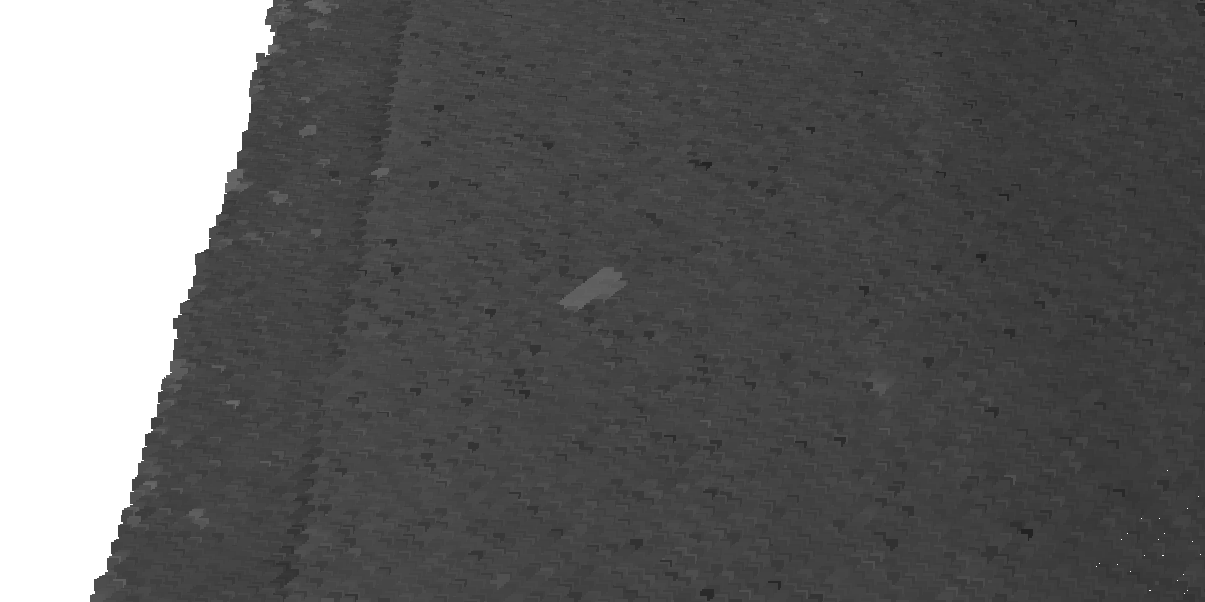
\includegraphics[width=0.3\textwidth]{graphics/fake_road_marking}
    \caption{Eine kleine Stelle auf der Straße, die eine ähnlich hohe Intensität wie Fahrbahnmarkierungen besitzt.}
    \label{fig:fake_road_marking}
\end{figure}

\subsection*{Koordinatenbasiert}

Es existieren verschiedene Maße, die für einen einzelnen Punkt die Form und Oberfläche seiner lokalen Nachbarschaft beschreiben \citep{Han.etal-2018}. Eine Auswahl dieser grundsätzlich einwertigen Features soll im Folgenden erläutert werden. \\
Die Basis jener Maße ist die Betrachtung der umgebenden 3D-Koordinaten eines Punktes und deren Verteilung. Dies wird repräsentiert durch die Kovarianzmatrix. Grundsätzlich beschreibt die Kovarianz zwischen zwei Variablen einen Grad ihres linearen Zusammenhangs: Ihr Vorzeichen deutet an, ob höhere Werte der einen Variable eher mit höheren oder niedrigeren Werten der anderen Variable einhergehen und umgekehrt. Im konkreten Fall von 3D-Daten sind die Variablen die drei Dimensionen \textit{X}, \textit{Y} und \textit{Z} selbst, die zusammen eine \textit{3×3}-Kovarianzmatrix einer Punktmenge bilden und in ihren Einträgen die Kovarianz zwischen den entsprechenden Dimensionen beschreibt. Die Durchschnitte der Variablen für die Zentrierung der Koordinaten sind hier die Koordinaten des durchschnittlichen Punkts der Menge, dem sogenannten \textit{Centroid}. \\
Ist diese Matrix für einen Punkt und seine Nachbarschaft einmal berechnet, müssen aussagekräfige Informationen daraus extrahiert werden. Für die genutzten Maße geschieht das mittels der drei Eigenwerte der Matrix. Diese bemessen die höchsten Varianzen entlang paarweise orthogonaler Achsen. Die Eigenwerte $\lambda_1$, $\lambda_2$ und $\lambda_3$ werden absteigend sortiert, sodass $\lambda_1 \geq \lambda_2 \geq \lambda_3$. Anschließend werden sie normalisiert durch Division ihrer Gesamtsumme: 
\begin{equation}
    \label{formula:eigen_normalization}
    e_i = \frac{\lambda_i}{\lambda_1 + \lambda_2 + \lambda_3}, i \in \{1, 2, 3\}.
\end{equation}
Die Berechnung der Eigenwerte ist aufwändiger als die der intensitätsbasierten Features. Zu diesem Zweck wurde der \texttt{EigenvalueCalculator} im \texttt{PCTool} implementiert. Dieser baut zu großem Teil auf dem zuvor existierenden \texttt{NormalsEstimator} auf, welcher für alle Punkte parallel ihre abgeschätzte Normale berechnet, die senkrecht auf der approximierten Oberfläche steht. Diese Normale ergibt sich als der Eigenvektor der Kovarianzmatrix mit dem kleinsten Eigenwert. Da in diesem Schritt also die Eigenwerte ohnehin berechnet werden, soll im \texttt{EigenvalueCalculator} beides kombiniert werden. Mit einstellbarem Scale werden die Normalen berechnet und jeweils drei Eigenwerte für alle Punkte zurückgegeben. Daraufhin werden diese entsprechend \ref{formula:eigen_normalization} normalisiert durch Division der Gesamtsumme. \\\\
Mittels der drei normalisierten Eigenwerte können nun die Maße \textit{Linearity}, \textit{Planarity}, \textit{Scattering} (auch \textit{Spherity}) sowie \textit{Local Curvature} (auch \textit{Change of Curvature}, folgend nur \textit{Curvature}) einfach berechnet werden, wie es in Tabelle \ref{table:eigenvalue_features} dargestellt ist. Diese Features werden unter anderem von \cite{Zaboli.etal-2019} und \cite{Li.Cheng-2018} genutzt, um städtische Objekte in \textit{Mobile-Mapping}-Punktwolken zu erkennen. Sie beschreiben, wie linear, eben oder rund die Nachbarschaft eines Punktes sich verhält und wie stark sie sich im Vergleich zu einer Ebene krümmt. Von ihrer Aussagekraft sind sie vergleichbar mit den in \cite{Zhiqiang.etal-2019} genutzten Features \textit{Roughness Index} und \textit{Gaussian Curvature}. Die Berechnung der Maße pro Punkt wird durchgeführt von Objekten der jeweils zuständigen Klasse (\texttt{CurvatureCollector} für \textit{Curvature}, usw.). \\

\begin{table}
\centering
\begin{tabular}{c|c|c|c}
Linearity & Planarity & Scattering & Curvature \\ 
$\frac{e_1 - e_2}{e_1}$ & $\frac{e_2 - e_3}{e_1}$ & $\frac{e_3}{e_1}$ & $\frac{e_3}{e_1 + e_2 + e_3}$ \\
\end{tabular}
\caption{Vier einwertige, auf den Eigenwerten der Kovarianzmatrix basierenden Features zur Beschreibung der Form der lokalen Nachbarschaft.}
\label{table:eigenvalue_features}
\end{table}

Auf Basis dieser einwertigen Features werden dann mehrwertige in Form von Histogrammen gebildet. Dabei hat sich jedoch herausgestellt, dass \textit{Linearity} und \textit{Planarity} nur einen geringen Informationswert bieten bezüglich der Unterscheidungskraft. Deshalb sind diese beiden Maße nicht Teil der koordinatenbasierten Features, sondern lediglich \textit{Scattering} und \textit{Curvature}. Im Experiment mit nur einwertigen Features werden alle vier Werte an die Featurevektoren angehängt. \\
Die Grenzen der Histogramm-Wertebereiche sind zusätzlich vom Scale abhängig, da die Varianz der Werte im kleinen Scale generell höher ist. So können im Radius von wenigen Zentimetern kleine Unterschiede der Koordinaten einen großen Einfluss auf den Wert haben, was auch an der geringen Zahl an Nachbarn liegt (siehe Tabelle \ref{table:neighbor_counts}). Für Scales von 10, 20 und mehr Zentimetern gleicht sich dies für die allermeisten Punkte wieder aus und die Werte nähern sich dem Durchschnitt der gesamten Punktwolke an. Beispielsweise ist der durchschnittliche Wert für \textit{Scattering} in der Trainingspunktwolke im Scale von 3$cm$ gleich 0,013, im Scale von 15$cm$ nur noch 0,001. Dabei ist der \textit{Scattering}-Wert für die hier behandelten Objektklassen ebenso wie die \textit{Curvature} grundsätzlich eher gering und weit entfernt vom maximalen Wert 1. Daher wird jeweils die Obergrenze des Histogramms - die durch manuelle Inspektion für eine gute Unterscheidung zwischen den Klassen festgelegt wurde - angepasst, was in Tabelle \ref{table:eigenvalue_features_impl} für die einzelnen Scales aufgeführt ist.

\begin{table}
\centering
\begin{tabular}{c|c|c|c|c|c}
& 3$cm$ & 6$cm$ & 9$cm$ & 12$cm$ & 15$cm$ \\
\hline
Scattering & 0,05 & 0,02 & 0,01 & 0,005 & 0,005 \\
Curvature  & 0,03 & 0,01 & 0,005 & 0,0025 & 0,0025 \\
\end{tabular}
\caption{Die Obergrenzen der linearen Histogramme von den genutzten Eigenwert-basierten Features für jeden Scale.}
\label{table:eigenvalue_features_impl}
\end{table}

In diesem Ansatz werden keine globalen Features verwendet, die jeweils die gesamte Punktwolke verarbeiten. Während etwa in \cite{Zhiqiang.etal-2019} \textit{Triangulated Irregular Networks} und Verfahren der \textit{Object Segmentation} genutzt werden, um die Umrisse von Objekten wie Schlaglöchern und Rissen zu detektieren, sollen hier nur lokale - also jeweils auf einen Scale beschränkte - Features Anwendung finden.
%!TEX root = foo-thesis.tex

\chapter{Uniqueness}
\label{chap:uniqueness}

Die zu klassifizierenden Objekte und deren einzelne Punkte sollten sich - im ein oder anderen Featureraum - merklich unterscheiden von den gewöhnlichen Straßenpunkten, die weder einen Schaden noch ein sonstiges besonderes Objekt darstellen. Dieses Konzept der \textit{uniquen} Punkte, teilweise auch \textit{key feature points}, hat das Ziel eine Punktwolke durch eine geeignete und angemessen große Menge von Punkten zu charakterisieren. \\
Da, wie bereits erläutert, die Features von verschiedenen Objekten teils erst bei verschiedenen Scales Unterscheidungskraft besitzen, gilt dies auch für die letztlich auf diesen Features basierende \textit{Uniqueness}. Daher wird jene pro Scale berechnet und jeder Punkt, der in mindestens einem Scale \textit{unique} ist, ist dies für die gesamte Punktwolke. Damit darüber hinaus bei stark unterschiedlichen Binzahlen der verschiedenen Featureräume - wenn etwa \textit{Curvature} doppelt so viele Bins hätte wie die Intensitätsdifferenzen - kein einzelner Featureraum einen zu starken Einfluss auf die Entscheidung zur \textit{Uniqueness} hat, wird letztere separat für jeden Featureraum berechnet. Sobald ein Punkt in mindestens einem Featureraum als \textit{unique} gilt, tut er dies auch für den gesamten Scale. Dieses Prinzip ist vor allem mit Blick auf potenzielle zukünftige Erweiterungen eingeführt worden, sollten zum Beispiel neue Features hinzukommen oder sich die Kennzahlen der Histogramme deutlich ändern. In der in diesem Ansatz genutzten Konfiguration, in der alle Histogramme dieselbe Größe besitzen, hat es geringe Auswirkungen. \\
Die Basis für die Ermittlung dieser \textit{uniquen} Punkte, wie vom Prinzip her auch in \cite{Rusu.etal-2008} genutzt, sind 
\begin{itemize}
    \item die Berechnung des Featureraums vom \textit{durchschnittlichen} Punkt (\textit{Mean})
    \item die Berechnung der Distanz zwischen dem Featureraum eines einzelnen Punktes und dem \textit{Mean}-Featureraum
\end{itemize}
Der \textit{Mean}-Featureraum kann für einwertige Features durch einfaches Bilden des Durchschnitts ermittelt werden, für mehrwertige Features werden die \textit{Counts} der einzelnen Bins über alle Punkte gleich gewichtet aufsummiert und entsprechend die \textit{Frequencies} neu berechnet. Umgesetzt wird dies durch die \texttt{mean}-Methode der \texttt{Histogram}-Klasse. \\\\
Diejenigen Punkte, die eine spezifizierte ausreichend große Distanz zum \textit{Mean} besitzen, werden anschließend als \textit{unique} betrachtet. Das genutzte Distanzmaß ist dabei die \textit{Kullback-Leibler-Divergenz (KL-Divergenz)} \citep{Kullback.Leibler-1951}. Dieses ist originär ein nicht-kommutatives Maß über zwei Wahrscheinlichkeitsverteilungen $P$ und $Q$ und drückt den Grad ihrer Verschiedenheit aus. In diesem Ansatz werden keine Wahrscheinlichkeitsverteilungen in jenem Sinne verwendet, doch die mehrwertigen Features in Form von Histogrammen erfüllen ihre nötige Eigenschaften: Alle Einträge, in diesem Fall die \textit{Frequencies} der Bins, liegen zwischen 0 und 1 und ihre Gesamtsumme beträgt genau 1. Für einwertige Features ist die zweite Eigenschaft nicht erfüllt, sie machen aber nur einen kleinen Teil der vollständigen Featurevektoren aus und werden aus Gründen der Praktikabilität dennoch identisch behandelt. \cite{Rusu.etal-2008} nutzen die KL-Divergenz ebenfalls als eines von mehreren getesteten Distanzmaßen. \\
$P$ steht hierbei jeweils für den Featureraum eines Punktes, $Q$ für den \textit{Mean}-Featureraum eines Scales. Die Formel zur Berechnung der Distanz zwischen diesen Featureräumen, wobei $P(i)$ und $Q(i)$ die \textit{Frequencies} der jeweils $i$-ten Bins und $n$ die Binzahl bezeichnen, lautet:
\begin{equation}    
    D(P || Q) = \sum_{i=1}^{n}{(P(i) - Q(i)) * \log_2\left(\frac{P(i)}{Q(i)}\right)}
\end{equation}
Die KL-Divergenz ist nur definiert, wenn für alle Einträge $i$ mit $Q(i)=0$ auch $P(i)=0$ gilt. Dies ist hier der Fall, da ein Eintrag von 0 im \textit{Mean} immer bedeutet, dass der entsprechende Eintrag auch beim Featureraum jedes Punktes gleich 0 ist. Für $P(i)=0$ ist der Summand als 0 definiert. \\
Von der Liste all der parallel berechneten Distanzen zum \textit{Mean} werden daraufhin der Durchschnitt $\mu$ sowie die Standardabweichung $\sigma$ ermittelt. Ein Punkt $P$ ist nun genau dann \textit{unique}, wenn gilt:
\begin{equation}
    D(P || Q) \geq \mu + \alpha * \sigma
\end{equation}
Dabei ist $\alpha$ ein im \texttt{PavementDistressDetector}-Knoten einstellbarer Parameter. Je größer dieser ist, desto weniger Punkte gelten tendenziell als \textit{unique} - diese sind dafür aber besonders auffällig. In den Experimenten hat sich generell ein Wert von 1,0 als annehmbar dargestellt. Eine Evaluierung verschiedener $\alpha$-Werte findet sich in Kapitel \ref{chap:eval}. \\\\
Die Gründe für eine solche Darstellung der Punktwolke durch eine geringere Zahl an Punkten sind vielfältig. Eine Motivation kann - gerade für statische Objekte - die Registrierung sein. Dabei sind die Ausgangslage zwei oder mehr Punktwolken, die durch mehrere Laserscannungen entstanden sind, etwa zu verschiedenen Zeitpunkten oder aus unterschiedlichen Perspektiven. Durch geeignete Algorithmen wie dem \textit{Sample Consensus Initial Alignment} \citep{Rusu.etal-2009} können für \textit{unique} Punkte der einen Punktwolke sogenannte Korrespondenz-Punkte in der anderen Punktwolke gesucht werden. Der Vorteil der Nutzung von \textit{Uniqueness} liegt hierbei darin, dass die Ausgangsmenge der zu betrachtenden Punkte für die Korrespondenzsuche drastisch, aber zugleich sinnvoll reduziert wird. Diese tiefgreifendere Verwendung des \textit{Uniqueness}-Konzepts wird in dieser Arbeit nicht näher behandelt, doch in Kapitel \ref{chap:outro} finden sich Ideen für seine Einsatzmöglichkeiten bei der Dokumentation von Straßenschäden. \\
Ein zweiter und pragmatischer Grund für die Ermittlung von \textit{uniquen} Punkten ist die resultierende Datenreduktion. Wie im vorherigen Kapitel erläutert, ist in der momentanen Architektur dieses Ansatzes eine Übertragung der Featurevektoren mit temporärer Festplattenspeicherung nötig. Da weiterhin die Nutzung von mehrwertigen Features wie Histogrammen inhärent zusätzlichen Speicheraufwand bedeutet, soll das \textit{Uniqueness}-Konzept Abhilfe schaffen. Ein weiterer Nebeneffekt ist die reduzierte Trainings- und \textit{Prediction}-Zeit des Modells, da weniger Eingaben zu verarbeiten sind. \\
Eine Bedingung für gute Ergebnisse der \textit{Uniqueness} ist in diesem Anwendungsfall, dass die Objekte von Interesse eine Minderheit der Punkte repräsentieren und so in der Gesamtpunktwolke entsprechend auffallen. Dies ist bei gewöhnlichen Punktwolken von Straßen der Fall, siehe Kapitel \ref{chap:eval} für Relationen der Klassen bei der Trainings- und Testpunktwolke. Für die nicht-\textit{uniquen} Punkte wird die implizite Annahme getroffen, dass diese den gewöhnlichen Straßenzustand repräsentieren, weshalb ihnen direkt die entsprechende Klasse zugewiesen wird. \\\\
Eine visuelle Darstellung des gesamten ersten Teils vom \textit{Feature-Extraction}-Ansatz, der Featureberechnung im \texttt{PavementDistressDetector}-Knoten, findet sich in Abbildung \ref{fig:feature_extraction}. 
Den Abschluss bildet dabei das Schreiben der sogenannten \textit{Featuresdatei}. Diese im Sinne der Speichereffizienz binäre Datei enthält die vollständigen Featurevektoren aller Punkte. Im Falle von betrachteter \textit{Uniqueness} sind nur die Vektoren der \textit{uniquen} Punkte geschrieben inklusive ihrer Indizes. Zusätzlich stehen immer zu Beginn die Gesamtzahl der folgenden Featurevektoren, die Anzahl der genutzten Scales sowie die Featurevektorgröße pro Scale. Die Featuresdatei wird anschließend von den Python-Skripten eingelesen und für Training und Test der Modelle bzw. die abschließende \textit{Prediction} der Klassen genutzt, siehe Kapitel \ref{chap:prediction}.

\begin{figure}[!ht]
    \centering
    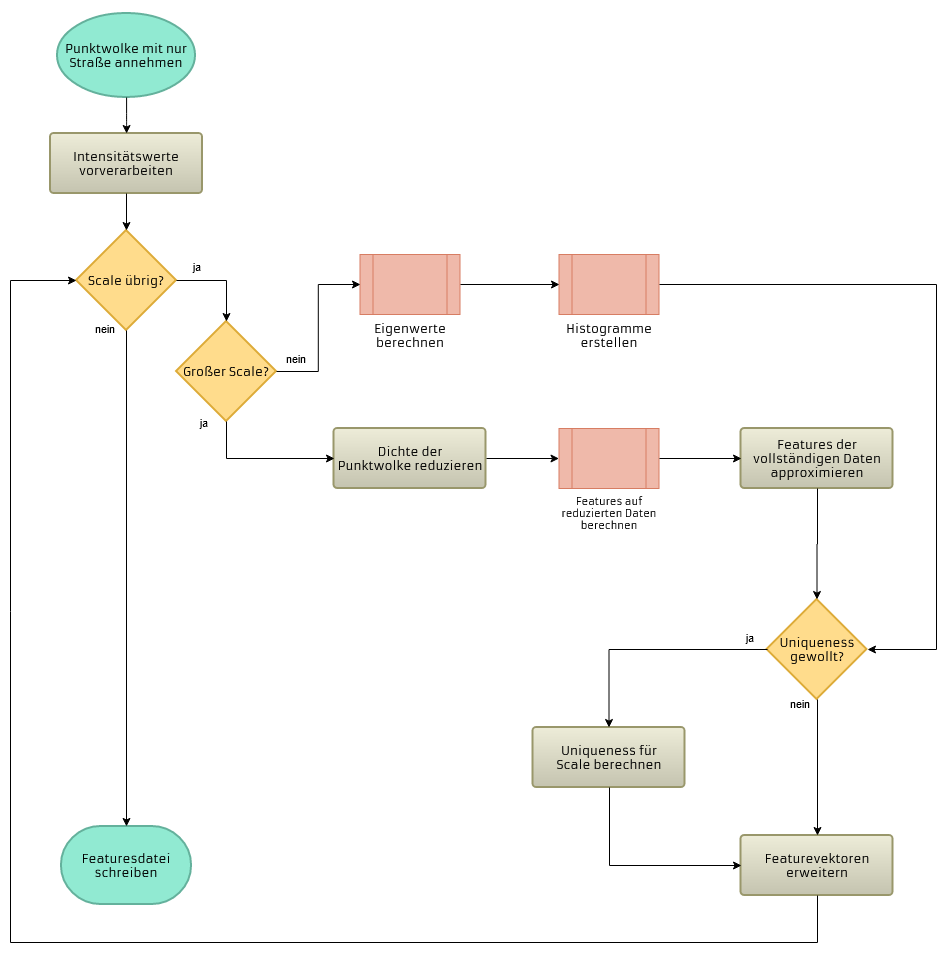
\includegraphics[width=0.98\textwidth]{graphics/flowchart_feature_extraction}
    \caption{Eine Übersicht des Ablaufs der Featureberechnung. Die roten Kästen kennzeichnen die bezüglich Laufzeit aufwändigsten Schritte des Prozesses.}
    \label{fig:feature_extraction}
\end{figure}
%!TEX root = foo-thesis.tex

\chapter{Prediction}
\label{chap:prediction}

Anhand der zuvor ermittelten Featurevektoren, bestehend aus Features mehrerer Scales und ggf. reduziert auf die Menge der \textit{uniquen} Punkte, soll nun jeweils die Klasse jedes Punktes vorhergesagt werden. Dazu kommt die zuvor geschriebene Featuresdatei zum Einsatz, aus der zunächst wieder die vollständigen Featurevektoren extrahiert werden müssen. Wie bei \cite{Zhiqiang.etal-2019} und \cite{Li.Cheng-2018} wird in diesem Ansatz für die \textit{Prediction} ein \textit{Random Forest} verwendet, der in dortigen Experimenten einen probabilistischen Ansatz sowie ein \textit{Support-Vector-Machine}-Modell übertroffen hat. Ein \textit{Random Forest} zeichnet sich grundsätzlich durch eine hohe Robustheit gegenüber kleinen Abweichungen oder Anomalien aus, die besonders bei feinen Features, wie sie hier vorkommen, wünschenswert ist. \\
Die Grundlage eines \textit{Random Forest} ist der \textit{Decision Tree}. Ein solcher einzelner Baum ist steuerbar über eine Menge von Parametern. Im Allgemeinen erhält er nur eine Teilmenge der Trainingsdaten und auch nur eine Teilmenge der Features zur Betrachtung. Anschließend wird er daraufhin trainiert, durch eine Reihe von Entscheidungen - im rein numerischen Fall basierend auf geeigneten Schwellwerten - die Klasse der Eingabe anhand der ihm zur Verfügung gestellten Features zu bestimmen. Um \textit{Overfitting}, also eine zu starke Spezialisierung auf die Trainingsdaten und damit zu geringe Generalisierung, zu vermindern, kann auch die maximale Anzahl an Entscheidungen - die Tiefe des Baums - festgelegt werden. \\
Für sich genommen ist ein einzelner Baum nur bei einigen Features zu einer sinnvollen Entscheidung für eine Klasse geeignet, bei anderen Features ist diese eher zufällig. Dies wird im \textit{Random Forest} dadurch ausgenutzt, dass jener oft aus Hunderten oder mehr unkorrelierten \textit{Decision Trees} besteht. Jeder von diesen trifft eine Entscheidung, die letztliche Entscheidung des gesamten Modells ergibt sich als Mehrheitsmeinung (\textit{Majority Vote}) dieser Einzelvorhersagen. Das Zusammenspiel aus \textit{Expertenmeinungen} jeweils spezialisierter Bäume und eher zufälligen Entscheidungen der restlichen Bäume ist einer der wesentlichen Gründe für die Stabilität des Modells \citep{Breiman-2001}.\\
Die einzigen beiden Parameter, die für diesen Ansatz manuell gesetzt wurden, sind die Gesamtzahl der \textit{Decision Trees}, aus denen der \textit{Random Forest} besteht, sowie die maximale Tiefe pro Baum. Die Anzahl der Bäume liegt für die Experimente bei 100. Es wurden auch höhere Zahlen getestet, die aber keine signifikanten Steigerungen bei der Qualität der \textit{Predictions} brachten. Während dieser Wert dem von \cite{Zhiqiang.etal-2019} gleicht, liegt die maximale Tiefe eines Baums hier bei 15 statt bei 10. Dies kann damit begründet werden, dass im vorliegenden Ansatz deutlich größere Featurevektoren genutzt werden: statt insgesamt 48 beinhalten sie hier 240 Werte (5 Scales á 48 \textit{Frequencies}). Eine noch größere Tiefe brachte bei Versuchen allerdings keine Verbesserungen mehr - im Gegenteil scheint dann ein \textit{Overfitting} auf die Trainingsdaten stattzufinden durch zu spezialisierte Entscheidungen pro Baum. \\
Um mit dem Ungleichgewicht der Klassen umzugehen, das in Tabelle \ref{table:class_frequencies} konkretisiert wird, findet für das Training ein \textit{Sampling} der gewöhnlichen Straßenpunkte statt. Das bedeutet, von allen Straßenpunkten wird ein zufälliger Anteil behalten, der dem \textit{Random Forest} übergeben wird. Der Anteil für die durchgeführten Experimente ist dabei so groß, dass jene Punkte, die nicht die Klasse Straße besitzen, etwa ein Zehntel der Gesamtpunkte ausmachen. Dies stellt eine Abwägung dar von der Reduktion des Ungleichgewichts gegenüber der Beibehaltung realistischer Klassenverhältnisse. \\\\
Für die \textit{Predictions} mittels \textit{Random Forest} wird das Paket \textit{scikit-learn} verwendet, das vielseitige Funktionalitäten im Bereich des maschinellen Lernens bietet. Die Python-Skripte des Ansatzes lassen sich über eine Kommandozeilen-Schnittstelle bedienen:
\begin{itemize}
    \item Es kann ein \textit{Random Forest} erstellt und trainiert werden. Dazu muss eine Featuresdatei eingelesen werden sowie eine Trainingspunktwolke mit den tatsächlichen Klassen. Darauf kann das Modell anschließend \textit{gefittet} werden, also seine Ausgaben an die gewünschten Ausgaben angenähert.
    \item Es kann ein \textit{Random Forest} getestet werden auf seine Qualität. Dazu muss neben dem trainierten Modell erneut eine Featuresdatei eingelesen werden sowie die zugehörige Testpunktwolke mit den tatsächlichen Klassen. Anschließend findet die \textit{Prediction} der Punktklassen durch den \textit{Random Forest} statt, was mit den erwarteten Klassen abgeglichen und in Form von Metriken pro Klasse evaluiert wird. Zu den hier verwendeten Metriken siehe Kapitel \ref{chap:eval}.
    \item Es kann auch ein anderes Modell auf seine Qualität getestet werden. Dazu wird neben der Testpunktwolke mit den tatsächlichen Klassen nur die \textit{Prediction}-Punktwolke benötigt mit den vorhergesagten Klassen. Damit werden anschließend ebenfalls Metriken für die einzelnen Klassen berechnet. Diese Option wurde vorrangig eingeführt, um mit den \textit{Predictions} von \texttt{PointNet} analog zu arbeiten wie mit denen des eigenen Ansatzes. Dies umfasst neben der Ermittlung derselben Metriken auch ein mögliches, identisch durchgeführtes \textit{Postprocessing}.
    \item Es können die Klassen einer noch nicht annotierten Punktwolke vorhergesagt werden. Dazu muss neben dem gewünschten Modell die entsprechende Featuresdatei eingelesen werden sowie die Punktwolke selbst zum Schreiben der Klassen. Dieser \textit{Prediction}-Teil ist für einen potenziellen regelmäßigen Einsatz auf der Plattform der bedeutsamste.
\end{itemize}
Beim Testen sowie der \textit{Prediction} des Modells besteht die Möglichkeit, über ein \textit{Flag} zu bestimmen, ob ein \textit{Postprocessing} der vorhergesagten Klassen stattfinden soll oder nicht. Genaue Erläuterungen zu dessen Funktionsweise finden sich in Kapitel \ref{chap:postproc}. In Abbildung \ref{fig:prediction} ist der grundsätzliche Ablauf einer solchen \textit{Prediction} dargestellt.

\begin{figure}[!ht]
    \centering
    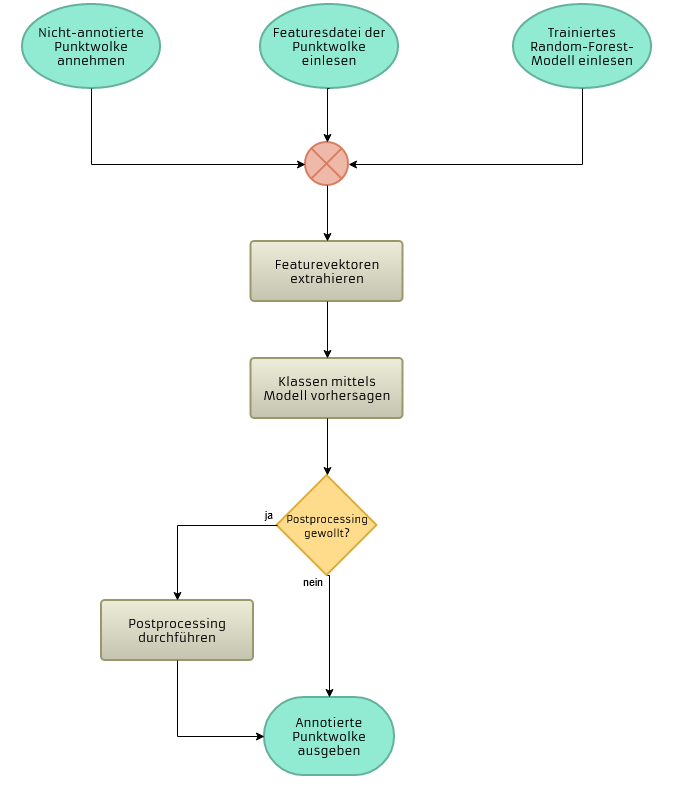
\includegraphics[width=0.95\textwidth]{graphics/flowchart_prediction}
    \caption{Eine Übersicht des Ablaufs einer Prediction.}
    \label{fig:prediction}
\end{figure}
%!TEX root = foo-thesis.tex

\chapter{Ansatz Deep Learning}
\label{chap:deepl}

\texttt{PointNet} \citep{Charles.etal-2017} ist eine \textit{Deep-Learning}-Architektur. Das neuronale Netz ist in der Lage eine Punktmenge zu verarbeiten, ohne von der Reihenfolge der Punkte abhängig zu sein. Dabei kann es sowohl einer gesamten Punktwolke eine Klasse zuweisen als auch die Punktwolke nach semantischen Klassen pro Punkt segmentieren. Da eine Implementierung von \texttt{PointNet} nicht Fokus dieser Arbeit ist, soll dessen Architektur nur grob zusammengefasst werden. Als wichtige Merkmale des Netzes werden genannt: 
\begin{itemize}
    \item das Nutzen einer symmetrischen Funktion für die permutationsunabhängige Prozessierung der Punkte
    \item die gleichzeitige interne Verwendung und Konkatenation von globalen Features und lokalen Features für die Berechnung der Gesamtklasse der Punktwolke oder der Einzelklassen der Punkte
    \item die automatische Angleichung der Koordinaten sowie Pro-Punkt-Features über Punktwolken hinweg, um eine Unabhängigkeit von Transformationen wie Rotation und Translation zu erreichen
\end{itemize}
Standardmäßig besteht der Input für \texttt{PointNet} lediglich aus den dreidimensionalen Punktkoordinaten. Allerdings lassen sich beliebige weitere Pro-Punkt-Features anhängen, was insbesondere für solche Attribute sinnvoll ist, die sich nicht indirekt aus den Koordinaten allein herleiten lassen. In dieser Arbeit gilt das für die Intensität, die auch im \textit{Feature-Extraction}-Ansatz genutzt wird. Entsprechend werden für einen aussagekräftigen Vergleich der Ansätze diese Werte den Koordinaten angehängt. \\
Auch die Arbeitsweise der beiden Ansätze bei der \textit{Prediction} unterscheidet sich: Statt sich Punkte einzeln anzuschauen, Features zu berechnen und eine Klasse vorherzusagen, wird bei der Nutzung von \texttt{PointNet} eine (durch Parameter in der Größe beeinflussbare) Menge von \textit{Samples} aus der gesamten Punktwolke gezogen. Für jeden dieser Punkte wird eine feste Zahl an Nachbarn bestimmt in ebenfalls fest eingestelltem (maximalen) Scale. Bei zu wenig Nachbarn werden Punkte mehrmals in die Menge aufgenommen. Nach Durchlaufen des Netzes wird jedem dieser Punkte auf einmal eine eigene Klasse zugewiesen, die das Modell für am wahrscheinlichsten hält. \\
Insgesamt lässt sich sagen, dass sich dieser modernere Ansatz - wie andere \textit{Deep-Learning}-Architekturen - dadurch auszeichnet, automatisch aussagekräftige Features aus dem \textit{Input} zu extrahieren. Dadurch wird ein grundsätzlich generischer Ablauf geschaffen, der nicht mehr auf manuell erarbeiteten und meist auf einen Anwendungsfall spezialisierten Features basiert, sondern für gute Ergebnisse lediglich ausreichend Trainingsdaten benötigt. \\\\
Da auf die Funktionsweise von \texttt{PointNet} hier kein Einfluss geübt werden kann, beschränken sich die Experimente auf die Nutzung verschiedener Parameterkombinationen. Die letztlich für die Klassifizierung relevanten Parameter des Modells bzw. für dessen Einsatz durch \texttt{PCNN} sind\footnote{https://gitlab.hpi3d.de/pcr/pcnn-docs/-/blob/main/latex/pcnn.pdf} folgende:
\begin{enumerate}
    \item der \textit{Query Radius}. Dieser Wert gibt an, wie weit ein Punkt maximal entfernt sein darf vom Ursprungspunkt, um zur Nachbarschaft zu gehören. Standardmäßig auf 3$m$ gesetzt für größere Objekte wie Häuser und Bäume, sollte er für den Anwendungsfall dieser Arbeit mit Blick auf die betrachteten Klassen entsprechend reduziert werden. Da nur ein fester Wert einstellbar ist, werden Experimente durchgeführt für jeden der im \textit{Feature-Extraction}-Ansatz genutzten Scales. In der Evaluierung wird dabei auch auf die Unterschiede in der jeweiligen Klassifikationsleistung eingegangen. 
    \item die \textit{Neighborhood Size}. Hiermit wird bestimmt, wie groß jede betrachtete Nachbarschaft ist. Weil auch dieser Wert für alle Punkte gleich bleibt, aber nicht jede Nachbarschaft dieselbe Punktanzahl enthält, muss unter Umständen aufgefüllt werden durch Mehrfachnutzung einzelner Punkte. Damit diese Ausnahmebehandlung nicht allzu häufig Anwendung findet, orientiert sich die genutzte Nachbarschaftsgröße in den Experimenten am jeweiligen \textit{Query Radius}. Genauer bedeutet dies, dass der Wert nahe der durchschnittlichen Nachbarzahl für den entsprechenden Scale liegt.
    \item der \textit{Length Divider}. Dieser \texttt{PCNN}-eigene Parameter hat einen Einfluss darauf, wie viele \textit{Samples} für das Training des Modells aus der Punktwolke gezogen werden. Je kleiner der Wert, desto mehr Punkte werden betrachtet und umgekehrt. Für \textit{Predictions} auf neuen Daten hingegen wird jeder Punkt als \textit{Sample} genommen und somit klassifiziert.
    \item die Anzahl an Epochen. Eine Epoche ist dann beendet, wenn alle Trainingsdaten - hier die Menge aller \textit{Samples} mit ihren jeweiligen Nachbarschaften - das Modell einmal durchlaufen haben. Mit mehr Epochen steigt grundsätzlich die Genauigkeit des Modells, das mit wenigen Epochen eher zufällige Ergebnisse bringt. Allerdings muss dabei beachtet werden, dass zu viele Epochen \textit{Overfitting} verursachen können, was sich dann in schlechteren \textit{Predictions} bei unbekannten Daten bemerkbar macht. Aus diesem Grund beendet \texttt{PCNN} das Training frühzeitig, sobald Epochen keine Verbesserung der Leistung mehr bringen.
\end{enumerate} 
Ergebnisse dieses Ansatzes und ein Vergleich mit denen vom \textit{Feature-Extraction}-Ansatz finden sich in Kapitel \ref{chap:eval}.
%!TEX root = foo-thesis.tex

\chapter{Postprocessing}
\label{chap:postproc}

Die Nachprozessierung findet statt, nachdem vom jeweiligen Ansatz alle Punkte einer Klasse zugewiesen wurden. Da dies eine verhältnismäßig simple Aufgabe ist, findet sich die Implementierung in denselben Python-Skripten, welche auch die Funktionalität zum Modelltraining und -test des \textit{Feature-Extraction}-Ansatzes beinhalten. Die Grundidee ist, Klassen von denjenigen Punkten noch einmal zu ändern, bei denen eine andere Klasse aufgrund der unmittelbaren Nachbarklassen wahrscheinlich ist. Dies geschieht in zwei Richtungen, wofür sequentiell zwei Iterationen notwendig sind. In beiden Richtungen wird eine Punktenachbarschaft im Scale von 7,5$cm$ betrachtet, die sich als geeignet herausgestellt hat. Auch hier wird für den effizienten Zugriff auf die Nachbarn ein zuvor für die Punktwolke ersteller \textit{k-d}-Baum genutzt, der an dieser Stelle entsprechend in Python implementiert ist. \\\\
Die erste Richtung besteht darin, Klassen-Außenseitern die Standardklasse der gewöhnlichen Straße zuzuweisen. Darunter fallen Punkte, die momentan nicht Straße sind, aber auch nicht genügend Punkte ihrer Klasse in unmittelbarer Umgebung haben. Für jede der betrachteten Objektklassen wird angenommen, aus mehr als einigen wenigen Punkten zu bestehen. Solche Klassifizierungen werden daher als eher zufälliges \textit{Rauschen} interpretiert und versucht zu beseitigen. \\
Der Klassenwechsel wird genau dann durchgeführt, wenn im Scale nicht mindestens 10\% der Punkte dieselbe Klasse wie der Ursprungspunkt besitzen. Dies funktioniert gut für Klassen, die wie der kugelförmige Scale auch rundlich sind, darunter Gullys und Schlaglöcher. Für Flickstellen kann dies problematischer sein, da diese meist dünn und linienartig verlaufen. Die Auswirkungen dieser Verarbeitung auf die verschiedenen Klassen finden sich in Kapitel \ref{chap:eval}. \\\\
Die andere Richtung behandelt Straßenpunkte, die inmitten von Nicht-Straßenpunkten liegen. Bei genügend großem Anteil von letzterer Gruppe nimmt der Punkt die häufigste Nicht-Straßenklasse seiner Nachbarschaft an. Auf diese Weise sollen zum Beispiel Schlaglöcher innen aufgefüllt oder die Mitte von Gullys ergänzt werden, wenn sie etwa wegen eines zu geringen Scales nicht als eben jene Klassen erkannt wurden. \\
Zunächst wird dazu über die als gewöhnliche Straße klassifizierten Punkte iteriert und jeweils der Prozentsatz an Punkten im Scale ermittelt, der nicht Straße ist. Übersteigt dieser die Schwelle von 50\%, wird dem Ursprungspunkt die häufigste Nicht-Straßenklasse seiner Nachbarschaft zugeteilt. Für eine weitere Zeitersparnis wird diese Iteration letztlich nur auf denjenigen Straßenpunkten ausgeführt, die in der Nachbarschaft mindestens eines Nicht-Straßenpunktes liegen, da auch nur jene für einen Klassenwechsel dieser Richtung in Frage kommen. Wegen des großen Überwiegens der Straßenpunkte sinkt durch diesen Schritt ihre noch zu betrachtende Menge beträchtlich. \\\\
Dieses \textit{Postprocessing} soll nur vermeintlich eindeutige Fehlklassifzierungen ausbessern. Den ursprünglichen Klassifizierungen, ob durch \texttt{PointNet} oder den eigenen Ansatz ermittelt, wird dabei wegen ihrer tiefergehenden Begründungen für die Entscheidung eine höhere Legitimation zugestanden. Daher wird die auf den erläuterten Heuristiken beruhende Nachverarbeitung mit eher zurückhaltenden Parametern ausgeführt, obwohl dies unter Umständen zur Beibehaltung von Außenseiterpunkten oder Straßenpunkten inmitten anderer Klassen führt.
%!TEX root = foo-thesis.tex

\chapter{Evaluierung}

\section{Trainings- und Testdaten}

% \section{Experimente}

\section{Preprocessing} 

\section{Ansatz Feature-Extraction} 

\subsection{Features}

\subsection{Scales}

\subsection{Ein- und mehrwertige Features} % hier darauf eingehen, dass durch Histogramme größere Scales erspart bleiben

\subsection{Uniqueness}

\subsubsection{Sonstige Verarbeitungsschritte} 

\subsubsection{Prediction per Random Forest} 

\section{Ansatz Deep Learning}

\section{Postprocessing}

% immer subsections mit (tlw. Vergleichen mittels) Bildern, Plots, Metrics und Performance PLUS Erklärungen/Vermutungen
% auch eingehen auf Speicherverbrauch (nicht nur Dauer) und Tradeoff dazwischen -> evtl. auch kleine Techniken zur Speicherreduktion (mehrere 0.0er Bins in Folge, ist auch weniger Noise)

% Kapitel noch anders strukturieren, mehr auf Vergleich aufbauen zwischen beiden Ansätzen
% PointNet mit gleichen Scales wie ich (einzelne ausprobieren und vergleichen mit Gesamtleistung von mir)
% PointNet: schauen, ob Parameter wie neighborhood size anzupassen sind

% zum Schluss nochmal alles probieren mit zusätzlichem Gehweg, Bordsteinkante plus Noise; je nach Ergebnissen darauf eingehen oder nicht...
% darauf eingehen, dass künstliche Schlaglöcher erzeugt?
%!TEX root = foo-thesis.tex

\chapter{Fazit und Ausblick}

\mediumtodo{Literaturverzeichnis korrigieren bzgl. Article/Inproceedings, Editors und Roberts Titel ergänzen}
\mediumtodo{Reihenfolge des Literaturverzechnis ordnen}

\mediumtodo{Fazit schreiben (inkl. kurzer Zusammenfassung)}
% hier Fazit \\\\

Für den Feature-Extraction-Ansatz bieten sich verschiedene Verbesserungen und Erweiterungen an. Zum einen könnte die Integration in ein einziges abgeschlossenes System vollzogen werden, vorzugsweise das PCTool, um den zusätzlichen Overhead von Datentransfers zu vermeiden. Für die Straßenextraktion, einer notwendigen Vorstufe für die Schadenserkennung, könnten elaboriertere Verfahren entwickelt werden, die den Anteil der reinen Straße gegenüber Gehweg und Noise weiter erhöhen. Diese können neben der bisherigen Punktdichtebetrachtung etwa auch auf der Erkennung von Bordsteinkanten als seitliche Grenzen basieren. \\
Ein großer Fokus könnte auf der Nutzung von noch aussagekräftigeren Features liegen, die ja die Basis aller Predictions sind. Das können sowohl Variationen der bisher genutzten Features sein - darunter fallen auch nicht-lineare Histogramme, welche die vorkommenden Werte besser abbilden können - als auch komplett andere Maße. Globale Features mit der gesamten Punktwolke als Ausgangslage können ebenfalls eingearbeitet werden und zusätzliche Informationen in die Featurevektoren bringen, die mit lokalen Nachbarschaften allein nicht auszudrücken sind. \\
Insbesondere für die Berechnung der uniquen Punkte dürfte eine initiale Ermittlung des groben Straßenzustands hilfreich sein. Dies könnte durch einen weiteren Fingerabdruck der Straßenpunktwolke repräsentiert werden und beispielsweise ausdrücken, ob es sich eher um eine Straße in der Innenstadt in sehr gutem Zustand handelt oder um eine marode Landstraße. Diese Information würde schließlich genutzt werden, um Parameter des Uniqueness-Konzepts sowie Ober- und Untergrenzen der Histogramme besser abzuschätzen und letztlich sowohl die ermittelte Uniqueness als auch die Predictions für die konkrete Punktwolke zu verbessern. Mit einer so verfeinerten Uniqueness könnte außerdem die Geschwindigkeit und Genauigkeit einer Registration gesteigert werden, die vor allem auf den beständigen Gullys basiert. In Verbindung damit ist auch eine Dokumentation der Zustandsentwicklung einer Straße denkbar: Anhand der Änderungen der uniquen Punkte, zuvorderst der Schadensklassen, über einen gewissen Zeitraum könnten Problemstellen ausgemacht und eventuell sogar prognostiziert werden. \\
Eine Fortführung der Schadenserkennung mittels Deep-Learning-Ansätzen ist ebenfalls denkbar. Dabei könnten zum einen noch mehr Konfigurationen von PointNet auf ihre Qualität getestet werden. Zum anderen wären auch gänzlich andere Architekturen interessant, die auf direkter Punktbasis arbeiten, wozu auch der Nachfolger von PointNet zählt. Allen Ansätzen gemein ist jedoch ein ausgereifteres Postprocessing, das seinen Fokus je nach Anwendungsfall anders legen könnte. Falls zum Beispiel Flickstellen besser und vollständiger erkannt werden sollen, können die einzelnen erkannten Cluster zu annähernd Rechtecken verbunden werden. Wenn hingegen vor allem die Detektion der Gullys relevant ist, kann mehr Aufwand betrieben werden, die Umrisse und das planare Innere präzise zu erkennen. \\
Wie generell für Machine-Learning-basierte Ansätze wären auch hier mehr und vor allem unterschiedlichere Trainingsdaten wichtig, um auf vielfältigen realen Daten gute Ergebnisse zu liefern. Dazu zählen etwa Schlaglöcher mit größeren Tiefen oder länglicheren Umrissen. Auch Gullys mit anderen Größen und weitere Klassen wie Risse oder sonstige Straßenobjekte könnten von Interesse sein. Außerdem würden bei weiteren Daten auch mehr verschiedene Scanner zum Einsatz kommen, wofür sich das Preprocessing der Intensitäten auszahlen sollte. Auf diese Weise könnte der bisherige \textit{Proof of Concept} erweitert werden, um die Vielfalt und Komplexität der Realität besser zu verarbeiten. \\
Schließlich könnte mit der Erkennung von Schäden und Unzulänglichkeiten einer Straße auch eine Bewertung ihres Zustands erfolgen. Dabei sind verschiedene Verfahren denkbar, etwa eine einfache Kumulation der Punkte pro Schadensklasse in der gesamten Punktwolke. Solche Schritte könnten jedoch auch in kleinerem Maßstab vorgenommen werden, indem mit gängigen Geoinformationssystemem gleichmäßige Raster in der Punktwolke erzeugt und einzeln bewertet werden. Je nach notwendiger Genauigkeit der Zustandsbewertung könnte die Klassifikation in feineren Abstufungen geschehen: So würden zum Beispiel Schlaglöcher anhand ihrer Größe und Tiefe eingeteilt werden in \textit{kleiner}, \textit{mittlerer} oder \textit{großer} Schaden. In jedem Fall wäre eine solche Bewertung kleinerer Abschnitte dazu geeignet, einfach Priorisierungen für Reparaturen zu schaffen und Straßenschäden somit schneller und effizienter zu beheben.

% %!TEX root = foo-thesis.tex

\chapter{Einleitung}

\section{Terminologie}

\section{Projektüberblick}

\section{Schwerpunkte des Bachelorprojekts}

\subsection{BA1}

\subsection{BA2}

\subsection{BA3}

\subsection{BA4}

\section{Einordnung in den Projektkontext} % hier wsh. Motivation

\section{Struktur der Arbeit}
% %!TEX root = foo-thesis.tex

\chapter{Verwandte Arbeiten}
\label{chap:rel-work}

An dieser Stelle sollen andere Arbeiten angeschnitten werden, die auch Objekterkennung in Punktwolken thematisieren und zum Teil verwandte Zielsetzungen haben.

\section{Objekterkennung in Punktwolken}

Die semantische Segmentierung von Punktwolken, das bedeutet die Einteilung der Punkte in verschiedene Klassen, ist ein in der Forschung intensiv behandeltes Gebiet, welches durch kontinuierliche Steigerung der Rechenkapazitäten zunehmend an Bedeutung gewonnen hat. Da die Punktwolken oftmals durch an Fahrzeugen angebrachten Laserscannern erfasst werden, liegt der Fokus vieler Arbeiten auf der Erkennung von städtischen Objekten, meist mit entsprechender Größe: Fassaden, Bäume, Dächer oder Laternen sind Beispiele dafür. Zu diesem Zweck kommen verschiedene Features pro Punkt zum Einsatz, die großteils einen geometrischen oder reflektivitätsbasierten Hintergrund haben. Darunter fallen die in der Einleitung erwähnten approximierten Normalen oder Krümmungswerte wie \textit{Curvature}, welche die Form der umgebenden Nachbarschaft beschreiben, aber auch Informationen zu der Stärke der Reflektivität eines Punktes \citep{Thomas.etal-2018, Zaboli.etal-2019}. Um die Klassifikation zu erleichtern und mit der teils hohen Varianz zwischen einzelnen Punkten umzugehen, werden in einigen Ansätzen die Punkte zunächst zu größeren Gruppen aggregiert und fortan als Einheit behandelt. In \cite{Vosselman-2013} beispielsweise werden dazu zunächst Segmente gebildet, die planare Flächen zusammenfassen sollen. In \cite{Han.etal-2018} findet sich eine chronologische Auflistung und Erläuterung von Features, die sowohl lokale als auch globale Charakterisierungen von Punktwolken ermöglichen sollen. Moderne Ansätze bauen häufig auf \textit{Deep-Learning}-Modellen auf, welche direkt auf drei- oder mehrdimensionalen Daten arbeiten und erwähnte Features eigenständig extrahieren sollen. Eine bekannte Architektur ist \texttt{PointNet}\cite{Charles.etal-2017}, welche in dieser Arbeit noch genauer vorgestellt und auch getestet wird. Bei \cite{Landrieu.Simonovsky-2018} werden hingegen \textit{Superpoint Graphs} gebildet, welche die Struktur einer Punktwolke und die Beziehungen zwischen Objekten in ihr kompakt repräsentieren sollen und auf denen anschließend ein \textit{Convolutional Network} operieren kann.

\section{Erkennung von Straßenschäden in Punktwolken}

Um mit der unregelmäßigen Struktur von Punktwolken umzugehen, basieren viele Verfahren der Erkennung von Straßenschäden auf bewährten Methoden. Eine Auflistung und Bewertung dieser findet sich bei \cite{Wenming.etal-2020}. Darunter fallen insbesondere Verfahren der Bildsegmentierung oder Kantenerkennungen (\textit{Edge Detection}). Darüber hinaus können auf von Punktwolken gemachten Bildern \textit{Convolutional Neural Networks} eingesetzt werden, die für die Nutzung auf regelmäßigen Bildern spezialisiert sind. Es existieren auch Ansätze, die Straßenschäden direkt in den Punktwolken erkennen wollen. Auf diese wird zum Teil noch mehrmals in der Arbeit verwiesen. Die Schwierigkeit besteht hierbei neben der Unstrukturiertheit von Punktwolken in den standardmäßig ungleichmäßigen Punktdichten. Einige aktuelle Ansätze wie \cite{Famili.etal-2021} und \cite{Gezero.Antunes-2019} setzen auf rein mathematische Herangehensweisen und komplexe geometrische Beschreibungen von Querschnitten der Fahrbahnoberfläche. Mit diesen Methoden sollen etwa Spurrillen ausfindig gemacht werden. Die Arbeiten von \cite{Li.Cheng-2018} und \cite{Zhiqiang.etal-2019} nutzen Verfahren des maschinellen Lernens, nämlich \textit{Random Forests}. Erstere der beiden Arbeiten setzt ihren Fokus nicht auf Straßenschäden, doch kann Bordsteinkanten erkennen und arbeitet darüber hinaus mit sogenannten \textit{Supervoxeln}, welche Punkte einer Nachbarschaft mit vergleichbaren Eigenschaften bündeln. \\\\
Der in dieser Arbeit entwickelte Ansatz baut auf einzelnen Features pro Punkt auf und beschränkt sich auf lokale Features, also solche, die nur eine begrenzte Nachbarschaft betrachten. Außerdem wird jeder Punkt unabhängig behandelt und seine Klasse vorhergesagt, es findet keine vorherige Aggregation von in bestimmten Eigenschaften \textit{ähnlichen} Punkten statt. Das gewählte Modell ist der \textit{Random Forest}, was in Kapitel \ref{chap:prediction} genauer begründet wird.
% %!TEX root = foo-thesis.tex

\chapter{Konzepte}

Das Ziel dieser Arbeit ist eine hinreichend genaue und effiziente Erkennung von Straßenschäden in 3D-Punktwolken auf Basis einzelner Punkte. Training und Evaluierung sind auf einer gescannten Asphaltstraße durchgeführt worden. Etwaige Bilder von Punktwolken oder Objekten in diesen entstammen der Trainings- oder Test-Punktwolke, die im Kapitel \textit{Evaluierung} genauer vorgestellt werden. Die grundlegenden Ideen und Techniken hinter den dafür nötigen Verarbeitungsschritten sollen in diesem Kapitel erläutert werden. Dabei wird sowohl auf den eigens konstruierten Ansatz per Feature-Extraction eingegangen als auch auf einen auf Deep Learning fußenden. Auch das beiden Ansätzen gemeine Pre- und Postprocessing wird kurz dargestellt.

\section{Betrachtete Objektklassen}

Entsprechend des Ziels nehmen Objekte, die auf einen mangelhaften Straßenzustand hinweisen, den vornehmlichen Fokus ein. Einfluss auf die Entstehung von Schäden verschiedener Art haben unter anderem der Niederschlag, temperaturbedingte Verformungen sowie die Verkehrsbelastung selbst.\footnote{https://www.ise.kit.edu/rd\_download/SBT/Kolloquium\_SBT\_2011-11-23\_C.Karcher.pdf} Es existieren Leitfäden\footnote{https://itzeb.heller-ig.de/leitfaden/} zur empfohlenen Auswertung solcher \textit{Substanzmerkmale}, an denen sich unter anderem bzgl. der verschiedenen Klassen orientiert wurde. Diese Klassen sind zum besseren Verständnis als Bilder der Punktwolke in Abbildung X dargestellt. \mediumtodo{Was anderes als Fußnoten nutzen?}\\
Darunter fallen insbesondere merkliche Absenkungen wie Schlaglöcher oder Risse. Schlaglöcher zeichnen sich durch lokale Höhenunterschiede, welche von mehreren Millimetern bis hin zu einigen Zentimetern reichen können, sowie ihre meist eher rundliche Form aus. Solche Absenkungen stellen gerade bei höheren Geschwindigkeiten und entsprechender Tiefe eine erhebliche Gefahr für die Kontrolle des Fahrzeugs und somit ein potenzielles Unfallrisiko dar. \\
% Unterschieden wird dabei zwischen \textit{aufgelegten} und \textit{eingelegten} Flickstellen, die auf die bestehende Fahrbahnoberfläche aufgebracht werden bzw. in die jeweils entnommene Decke wieder hineingelegt werden.
Auch Flickstellen bilden eine interessante Klasse: Sie werden angebracht, um beschädigte Straßenteile - wie zum Beispiel ein Schlagloch - zu überdecken und auf diese Weise ungefährlich zu machen. Charakterisiert werden sie durch ihre wegen der maschinellen Fertigung meist rechteckige Struktur sowie der im Vergleich zur unmittelbaren Umgebung oft dunkler erscheinenden Fugendichtmasse. Letztere kann durch Überquellen ebenfalls für marginale Höhenunterschiede sorgen. Auch wenn Flickstellen selbst also keinen Schaden darstellen, ist ein Straßenabschnitt, der zu großen Teilen von Flickstellen überzogen ist, ein möglicher Hinweis auf eine sinnvolle Komplettreparatur. \\
Gullys und Kanaldeckel kommen in vielen Ausprägungen bezüglich Größe und Form daher. Obwohl diese selbstverständlich begründet angelegt wurden, zeichnen auch sie sich durch charakteristische Höhenunterschiede aus, was einen Vergleich unter anderem mit Schlaglöchern und somit eine genauere Betrachtung wert ist. Ein zuverlässiges Erkennen von Gullys kann außerdem, wie im Unterabschnitt \textit{Uniqueness} sowie im Kapitel \textit{Fazit und Ausblick} erwähnt wird, einen weiteren Vorteil bringen: Aufgrund ihrer beständigen Struktur können mehrere Scans desselben Straßenabschnitts zueinander ausgerichtet werden. Damit könnte etwa die Veränderung des Straßenzustands in einem bestimmten Zeitraum dokumentiert werden. \\
Eine weitere Auffälligkeit sind besonders dunkle, unregelmäßige und teils sehr große Flecken. Ohne genauen Anblick vor Ort ist nicht zweifelsfrei auszumachen, worum es sich handelt: Bindemittelaustritte sind eine Alternative, aber auch Ölflecken sind möglich und, durch die Nähe zu Parkplätzen, hier auch plausibel. Frische Ölflecken allerdings stellen augrund der geringen Griffigkeit eine große Rutschgefahr dar. Wegen dieser Option werden auch jene Stellen gesondert behandelt; der Einfachheit halber ist in der Arbeit folgend die Rede von Ölflecken. \\
Von der entgegengesetzten Intensität, aber für den sicheren Straßenverkehr unerlässlich, sind Fahrbahnmarkierungen. Durch ihre Materialzusammensetzung sollen sie sich zu allen Tageszeiten und Wetterbedingungen stark abheben vom Rest der Fahrbahn und so Orientierung bieten. Von Interesse könnte hier insbesondere sein, ob und welche Markierungen sich stellenweise durch Verschleiß nicht mehr ihrem Zweck gemäß genug abheben und einer Auffrischung oder Erneuerung bedürfen. \\\\
Andere Arbeiten wie \cite{Zhiqiang.etal-2019} und \cite{Famili.etal-2021} haben sich vollständig auf Höhenunterschiede vielfältiger Art konzentriert. Dazu zählen nicht nur Schlaglöcher, sondern auch feine Risse, Spurrillen oder Unebenheiten der Straße auf Quer- und Längsseite um wenige Prozent, die unter Umständen über mehrere Meter gemessen werden. Dies waren keine Ziele der Arbeit, entweder aus Mangel an geeigneten und ausreichenden Daten oder, da andere Verfahren besser geeignet erscheinen. Für die Berechnung dieser Quer- wie Längsunebenheit beispielsweise existieren Empfehlungen der * \mediumtodo{hier vllt. was von der Stadt Essen}. Diese beschreiben imaginäre Holzlatten, welche in regelmäßigen Abständen quer zur und längs der ebenfalls gescannten Straße gelegt werden. Anhand der Höhendifferenzen der Lattenenden können die gesuchten Werte mathematisch präzise ermittelt werden, ebenso andere Kenngrößen wie die Spurrinnentiefe oder fiktive Wassertiefe. \cite{Famili.etal-2021} verfolgen ähnliche Ansätze über Funktionsgraphen von Querschnitten der Oberfläche. Solche geometrischen Verfahren sind bereits verhältnismäßig akkurat und zuverlässig. \\ 
Die Schäden dieser Art spielen auch eine Rolle bei der Straßenzustandsbewertung. Daher könnten jene Verfahren kombiniert werden mit Ansätzen, die für die Erkennung von unregelmäßigen Schäden der Fahrbahnoberfläche spezialisiert sind, wie es die in dieser Arbeit getesteten sein sollen. Auf diese Weise kann erst ein gesamtheitliches Bild des Straßenzustands geschaffen werden.

\section{Preprocessing}

Die Schadenserkennung wird nicht unmittelbar auf der ursprünglich eingehenden Punktwolke (nachfolgend \textit{Input}) ausgeführt, sondern zuerst auf geeignete Weise vorprozessiert.
Die erste Aufgabe besteht darin, den Boden des Inputs zu bestimmen, um die Menge der potenziell interessanten Punkte für diesen Anwendungsfall zu reduzieren. Dazu wird eine Bodenerkennung (\textit{Ground Detection}) eingesetzt, welche unter anderem mit Höhenmodellen arbeitet. Schließlich werden die als Boden erkannten Punkte mit der entsprechenden semantischen Klasse markiert. In der Pipeline dieser Arbeit wird eine Ground Detection eingesetzt, die für den jeweiligen Input optimierte Parameter nutzt. Diese werden im Voraus - als anderes Teilsystem des Projekts - ermittelt anhand der Oberflächeneigenschaften des Inputs. Dadurch soll möglichst der komplette Boden, also insbesondere die vollständige Straße, und möglichst wenig an restlichen Punkten erfasst werden. \\\\
Mit diesen Informationen geht es dann an den Schritt, der die Straße selbst erkennen soll. Diese Street Detection soll also außenstehenden Rasen, niedrige Häuserwände und sonstige als Boden klassifizierte, aber nicht zur Fahrbahn selbst gehörenden Bereiche (\textit{Noise}) entfernen. Dabei wird vor allem mit der relativen Dichte der Punkte und einer darauf basierenden Abschätzung der Trajektorie des Scannerfahrzeugs gearbeitet. Dies beruht auf der Annahme, dass durch die Arbeitsweise der Scanner nahegelegene Oberflächen deutlich dichter abgetastet werden als weiter entfernte. Die Street Extraction baut auf einer zumindest größtenteils gelungenen Ground Detection auf. Sobald die nun als Straße erkannten Punkte extrahiert sind, beginnt der jeweilige Ansatz auf seine Weise, die oben genannten Klassen in der verbliebenen Punktwolke zu erkennen. \\\\
Zunächst erfolgt jedoch noch eine Wertenormalisierung. Während der Deep-Learning-Ansatz seine eigene Art der Normalisierung vornimmt, geht der Feature-Ansatz folgendermaßen vor: Das Intensitätsattribut besitzt eine hohe Varianz bezüglich verschiedener Laserscanner, die unter anderem von deren unterschiedlicher Technik oder Verarbeitung verursacht wird. Zwar liegt der Wertebereich des Attributs grundsätzlich bei 0 bis 65535, wird aber oftmals nicht ausgenutzt. Der Intensitätswert desselben Punktes, aufgenommen von zwei verschiedenen Scannern, kann sich um mehrere Tausend unterscheiden. Aus diesem Grund werden diese absoluten Werte zunächst in relative umgewandelt, sodass sie über verschiedene Punktwolken hinweg vergleichbar sind. \\
Ein weiterer Aspekt, der sich negativ auf die Normalisierung auswirken kann, sind einzelne Punkte, deren Intensität übermäßig stark von der Mehrheit der anderen Werte abweicht. Unabhängig davon, ob dies Messungenauigkeiten sind oder tatsächlich einzelne Abweichler, ist ein Entfernen dieser Werte erstrebenswert. Da aber natürlich auch diese Punkte erhalten bleiben und eine Intensität besitzen sollen, werden diese Außenseiter-Punkte noch vor der Normalisierung bestimmt und ihre Intensität auf den niedrigsten bzw. höchsten Wert gesetzt, der nicht zu den abweichenden Werten gezählt wird. Auf diese Weise sollen die Relationen zwischen verschiedenen Punktwolken erhalten bleiben, ohne durch die Werteanpassung und -normalisierung einen merklichen Informationsverlust zu erleiden bzgl. der hier betrachteten Klassen. \\
Da bei den 3D-Koordinaten keine so erheblichen Unterschiede zu erwarten sind, werden diese Werte nicht normalisiert und alle letztlich daraus ermittelten Features als vergleichbar über verschiedene Punktwolken hinweg angesehen.

\section{Ansatz Feature-Extraction}

Der Ansatz über die Feature-Extraction in seiner momentanen Form gliedert sich grob in zwei Teilschritte: Zunächst erfolgt die Ermittlung der Pro-Punkt-Features selbst, was den deutlich zeitintensiveren Anteil ausmacht. Anschließend erfolgt die Vorhersage (\textit{Prediction}) der Klassen allein auf Basis dieser berechneten Featurevektoren über einen Random Forest, ggf. reduziert auf eine Menge von in diesen Werten besonders auffälligen Punkten (siehe Abschnitt \textit{Uniqueness}). Dieses Vorgehen entspricht somit dem klassischen Machine-Learning-Prozess.

\subsection{Features}

Bei einer manuellen Feature-Bestimmung stellt sich zuerst die Frage, welche Features überhaupt in Betracht gezogen werden. Daher sollen nun grundsätzliche Features erläutert werden, die gewisse Unterscheidungsmerkmale zwischen den verschiedenen Klassen ausdrücken. \\
Die reine Intensität, also ein Maß zur Ermittlung der Stärke des reflektierten Lasers \mediumtodo{Paper?}, hebt bereits Fahrbahnmarkierungen durch einen sehr hohen und Ölflecken durch einen sehr niedrigen Wert hervor. \cite{Zhiqiang.etal-2019} nutzen dieses Attribut ebenfalls als Teil ihrer Featurevektoren, wobei dort noch eine Interpolation über Gewichtungen invers zur Distanz vorgenommen wird. Da der eine Wert scale-unabhängig ist und es auch einzelne Punkte mit diesen extremen Ausschlägen gibt (siehe Abbildung Y), die weder zur einen noch zur anderen Klasse gehören, wird an dieser Stelle eine Abhängigkeit vom Scale geschaffen: Beispielsweise kann der Durchschnitt der Nachbarschaftsintensitäten berechnet werden. Im kleinen Scale mögen diese Werte sich auch für Ausreißerstellen ähneln, im größeren Scale aber gleicht sich das für diese aus und bleibt etwa für Fahrbahnmarkierungen charakteristisch hoch. \\
Ebenfalls auf dem Intensitätsattribut beruhend ist eine Betrachtung der lokalen Intensitätsunterschiede der Nachbarn zum jeweils betrachteten Punkt. Neben Fahrbahnmarkierungen und Ölflecken sind gerade Flickstellen dadurch gekennzeichnet, dass die deutlich dunklere Fugendichtmasse, die Streifen mit wenigen Zentimetern Breite bildet, sich abhebt vom Rest der umliegenden Oberfläche und somit die meist rechteckige Form erkennen lässt. Auch Schlaglöcher besitzen oft, bedingt durch den bei ihnen abgetragenen Asphalt, eine geringere Intensität. Diese Differenzen sollen also dabei helfen, in ihrer Intensität auffällige Stellen einzugrenzen und zu erkennen. \\\\
% später evtl. noch reine Nachbarintensities dazunehmen sowie Elevation Differences / Roughness Index / Principal bzw. Gaussian Curvature
Neben diesen in unterschiedlichen Formen auf der Intensität basierenden Features werden natürlich auch die 3D-Koordinaten der Punkte genutzt. Es existieren verschiedene Maße, die für einen einzelnen Punkt die Form und Oberfläche seiner lokalen Nachbarschaft beschreiben. Eine Auswahl dieser grundsätzlich einwertigen Features soll im Folgenden erläutert werden. \\
Die Basis jener Maße ist die Betrachtung der umgebenden Koordinaten eines Punktes und deren Verteilung. Dies wird repräsentiert durch die Kovarianzmatrix. Grundsätzlich beschreibt die Kovarianz zwischen zwei Variablen einen Grad ihres linearen Zusammenhangs: Ihr Vorzeichen deutet an, ob höhere Werte der einen Variable eher mit höheren oder niedrigeren Werten der anderen Variable einhergehen und umgekehrt. Im konkreten Fall von 3D-Daten sind die Variablen die drei Dimensionen \textit{X}, \textit{Y} und \textit{Z} selbst, die zusammen eine 3×3-Kovarianzmatrix einer Punktmenge bilden, welche in den entsprechenden Einträgen die jeweilige Kovarianz zwischen den Dimensionen beschreibt. Die Durchschnitte der Variablen für die Zentrierung der Koordinaten sind in diesem Fall die Koordinaten des durchschnittlichen Punkts der Menge, dem sogenannten \textit{Centroid}. \\\\
Ist diese Matrix für einen Punkt und seine Nachbarschaft einmal berechnet, müssen nun sinnvolle Informationen daraus extrahiert werden. Für die genutzten Maße geschieht das mittels der drei Eigenwerte der Matrix. Diese bemessen die höchsten Varianzen entlang paarweise orthogonaler Achsen. Der zum geringsten Eigenwert zugehörige Eigenvektor repräsentiert dabei die Normale zur Punktmenge, welche senkrecht auf deren approximierter Oberfläche steht. \\
Diese Eigenwerte $\lambda_1$, $\lambda_2$ und $\lambda_3$ werden absteigend sortiert, sodass $\lambda_1 \geq \lambda_2 \geq \lambda_3$. Anschließend werden sie normalisiert durch Division ihrer Gesamtsumme: 
\begin{equation}
e_i = \frac{\lambda_i}{\lambda_1 + \lambda_2 + \lambda_3}, i \in \{1, 2, 3\}.
\end{equation}
Mittels dieser drei Werte können nun die gesuchten Maße \textit{Linearity}, \textit{Planarity}, \textit{Scattering} (auch \textit{Spherity}) sowie \textit{Local Curvature} (auch \textit{Change of Curvature}, folgend nur \textit{Curvature}) einfach berechnet werden, wie es in Tabelle \ref{table:eigenvalue_features} dargestellt ist. Diese Features werden unter anderem von \cite{Zaboli.etal-2019} genutzt, um städtische Objekte von Mobile-Mapping-Punktwolken zu erkennen. Sie beschreiben, grob formuliert, wie linear, eben oder rund die Nachbarschaft eines Punktes sich verhält und wie stark sie sich im Vergleich zu einer Ebene krümmt. Von ihrer Aussagekraft sind sie vergleichbar mit den in \cite{Zhiqiang.etal-2019} genutzten Features \textit{Roughness Index} und \textit{Gaussian Curvature}. Im Gegensatz dazu werden in diesem Ansatz aber keine globalen Features verwendet, die jeweils die gesamte Punktwolke verarbeiten. Während etwa \cite{Zhiqiang.etal-2019} \textit{Triangulated Irregular Networks} und Verfahren der \textit{Object Segmentation} dazu nutzen, um die Umrisse von Objekten wie Schlaglöchern und Rissen zu detektieren, sollen hier tatsächlich nur lokale, also jeweils auf einen Scale beschränkte, Features genutzt werden.

\begin{table}
\centering
\begin{tabular}{c|c|c|c}
Linearity & Planarity & Scattering & Curvature \\ 
$\frac{e_1 - e_2}{e_1}$ & $\frac{e_2 - e_3}{e_1}$ & $\frac{e_3}{e_1}$ & $\frac{e_3}{e_1 + e_2 + e_3}$ \\
\end{tabular}
\caption{Die vier einwertigen, auf den Eigenwerten der Kovarianzmatrix basierenden Features zur Beschreibung der Form der lokalen Nachbarschaft.}
\label{table:eigenvalue_features}
\end{table}

\subsection{Scales}

Um einen Punkt zu charakterisieren, wird seine lokale Nachbarschaft betrachtet. Für die Ermittlung der Nachbarschaft gibt es grundsätzlich zwei Wege: die \textit{k} nächsten Nachbarn zu nehmen oder alle Nachbarn, die im vorgegebenen Radius einer Kugel um den Ursprungspunkt liegen. Der Vorteil an den k Nachbarn ist, dass man sich über die betrachtete Nachbarzahl sicher sein kann. Allerdings hängt der dabei betrachtete Radius erheblich von der lokalen Punktdichte ab: Beim Mobile-Mapping wird für Punkte auf der Trajektorie des Scannerfahrzeugs mit demselben k also ein deutlich geringerer Radius betrachtet als für Punkte näher am Rand, siehe Abbildung X. Deshalb eignet sich die Radiusbetrachtung besser für konsistente und über verschiedene Punkte vergleichbare geometrische Features \citep{Thomas.etal-2018}. Diese Art der Nachbarschaftsbetrachtung - von nun an werden die Radii \textit{Scales} genannt - findet in dem Ansatz entsprechend Verwendung. \\\\
Die nächste Frage ist, welche konkreten Scales genutzt werden. Dass überhaupt die Nutzung mehrerer Scales sinnvoll ist, zeigt sich beim Blick auf verschiedene Objekte, die es zu erkennen gilt. Zum einen sind natürlich gerade Schlaglöcher besonders unregelmäßige Strukturen, die in vielerlei Ausprägungen vorkommen können: über mehrere Größen hinweg sowie Formen von sehr rund bis eher länglich. Flickstellen zeichnen sich vorzugsweise in kleinem Scale aus durch ihre hohen Intensitätsunterschiede. Bei größeren Gullys wird der innere, mittige Bereich aber erst mit deutlich größerem Radius auffällig, denn im kleinen Bereich ist dieser sehr planar. Um mit diesen verschiedenen Granularitäten umgehen zu können, werden mehrere, an typische Objektgrößen angepasste, Scales genutzt.
% hier Bild der eingefärbten Nachbarn nach kNN und nach Scale

\subsection{Ein- und mehrwertige Features}

Als Features für Punkte kommen zum einen einwertige Daten in Betracht. Das können direkt Attribute sein wie die Intensität, Werte, die sich aus der Punktenachbarschaft ergeben wie Curvature, oder kumulierte Formen davon wie Durchschnitte oder Standardabweichungen. \\
Daneben gibt es auch die Möglichkeit für mehrwertige Features. Diese können etwa als Histogramme ausgedrückt werden, also Häufigkeitsverteilungen für bestimmte numerische Merkmale. Sie sind zusammengesetzt aus mehreren sogenannten Bins, welche die Anzahl der Observationen zählen, die in den von ihnen aufgespannten Wertebereich fallen. In dieser Arbeit entspricht eine Observation dem Merkmal eines Punktes, etwa einem Curvature-Wert. Histogramme können linear sein, wenn alle Bins einen identisch großen Wertebereich haben, oder entsprechend nicht-linear, wobei in diesem Ansatz nur von linearen Histogrammen Gebrauch gemacht wurde, wie im Kapitel \textit{Implementierung} nachzuvollziehen ist. \\\\
Der Vorteil der Histogramme besteht in einer grundsätzlich höheren Aussagekraft durch die genauere Charakterisierung der Nachbarschaft \citep{Rusu.etal-2008}: Was sich etwa in einem Durchschnittswert durch entgegengesetzte Größen aufheben würde, kann nun präziser dargestellt werden. Mehr und damit feinere Bins, d.h. jeweils kleinere Wertebereiche, haben eine potenziell höhere Aussagekraft. Allerdings resultiert dies unter Umständen in einer zu starken Verteilung der Häufigkeiten, sodass charakteristische Ausschläge verloren gehen. Histogramme bieten aber noch weitere Vorteile: Die oben angesprochenen teilweise erheblichen Unterschiede der Dichte an verschiedenen Stellen einer Mobile-Mapping-Punktwolke machen einwertige Features unter Umständen schwierig vergleichbar für einen festen Scale. Bei Histogrammen kann dieser Fakt abgeschwächt werden, da durch das Einsortieren in Bins die Werte normalisiert werden in den Bereich von 0 bis 1, und zwar unabhängig von der Anzahl der Nachbarn. Deswegen werden im Ansatz zum Vergleich zwischen Histogrammen und auch für die Prediction lediglich die relativen Bingrößen (\textit{Frequencies}) betrachtet. Ferner wird auch der Umgang mit Außenseiterpunkten (\textit{Outliern}), die teilweise von Messungenauigkeiten stammen, erleichtert: Während sie im einwertigen Fall ein Feature stark verzerren können, erhöhen sie beim Histogramm nur die Frequency eines Bins leicht und sind somit beinahe wie leere Bins zu behandeln. Ähnliches gilt für Werte mit hoher Varianz, wie es vor allem die gemessene Intensität ist. Schließlich sind die Histogramme, im Gegensatz zu einigen anderen lokalen Deskriptoren \citep{Han.etal-2018}, unabhängig von Transformationen der Punktwolke wie Rotation oder Translation. \\
Für diesen Ansatz werden Histogramme genutzt bei den Features zur geometrischen Oberflächenbeschreibung sowie den Intensitätsunterschieden. In den Kapiteln \textit{Implementierung} und \textit{Evaluierung} wird darauf eingegangen, mit welchen Wertebereichen und Binzahlen gearbeitet wird bzw. was dies für Auswirkungen hat auf die Unterscheidbarkeit zwischen den Klassen. Grundsätzlich wird aber eine Kombination aus ein- und mehrwertigen Features eingesetzt. Zusammengehörige einwertige Features sowie einzelne Histogramme eines Attributs werden künftig teilweise als \textit{Featureräume} bezeichnet, etwa als Curvature-Featureraum.

\subsection{Uniqueness}

Die zu klassifizierenden Objekte und deren einzelne Punkte sollten sich - im ein oder anderen Featureraum - merklich unterscheiden von den gewöhnlichen Straßenpunkten, die weder einen Schaden noch ein sonstiges besonderes Objekt darstellen. Dieses Konzept der \textit{uniquen} Punkte, teilweise auch \textit{key feature points}, hat das Ziel eine Punktwolke durch eine geeignete und angemessen große Menge von Punkten zu charakterisieren. \\
Die Basis für die Ermittlung dieser uniquen Punkte sind, wie vom Prinzip her auch in \cite{Rusu.etal-2008} genutzt, die Berechnung einer Featurerepräsentation des \textit{durchschnittlichen} Punktes (\textit{Mean}) sowie der Distanz der Repräsentation einzelner Punkte zu diesem Durchschnitt. Diejenigen Punkte, die eine spezifizierte ausreichend große Distanz besitzen, werden als unique betrachtet. \\
Die durchschnittliche Repräsentation kann für einwertige Featureräume durch einfaches Bilden des Durchschnitts ermittelt werden, für mehrwertige Featureräume (Histogramme) werden die jeweiligen Bins über alle Punkte aufsummiert und entsprechend die Frequencies neu berechnet. Die Distanz von der Punktrepräsentation zur Meanrepräsentation kann dann über ein geeignetes Distanzmaß berechnet werden. Bei Betrachtung aller Distanzen können anschließend die entferntesten Punkte bestimmt werden. \\\\
Die Gründe für eine solche Darstellung der Punktwolke durch eine geringere Zahl an Punkten sind vielfältig. Eine Motivation kann - gerade für Objekte, für die eher nicht erwartet wird, sich zu verändern oder zu bewegen - die Registration sein. Dabei sind die Ausgangslage zwei oder mehr Punktwolken, die durch mehrere Scans entstanden sind, etwa zu verschiedenen Zeitpunkten oder aus unterschiedlichen Perspektiven. Durch geeignete Algorithmen wie dem \textit{Sample Consensus Initial Alignment} \citep{Rusu.etal-2009} können für unique Punkte des einen Scans sogenannte Korrespondenz-Punkte im anderen Scan gesucht werden, welche die jeweils ähnlichste Featurerepräsentation besitzen. Aus diesen Paaren kann die nötige Transformation zwischen den Punktwolken bestimmt und durchgeführt werden. Durch ein entsprechendes Fehlermaß, etwa über die paarweisen Distanzen, kann die Qualität dieser Annäherung ermittelt und nach dem geringsten Fehler optimiert werden, bevor eine abschließende Verfeinerung dieses \textit{Alignments} zum Beispiel über nicht-lineare Verfahren erfolgt. Der Vorteil der Nutzung von uniquen Punkten liegt hierbei darin, dass die Ausgangsmenge der zu betrachtenden Punkte für die Korrespondenzsuche drastisch, aber zugleich sinnvoll reduziert wird. Die tiefgreifendere Verwendung des Uniqueness-Konzepts wird in dieser Arbeit nicht näher behandelt, doch im Kapitel \textit{Fazit und Ausblick} wird noch einmal angerissen, inwiefern damit potenziell Änderungen des Straßenzustands im Verlaufe der Zeit ermittelt werden könnten. \\
Ein zweiter und pragmatischer Grund für die Ermittlung von uniquen Punkten ist die resultierende Datenreduktion. Wie im Kapitel \textit{Implementierung} genauer erläutert wird, ist in der momentanen Architektur dieses Ansatzes eine Übertragung der Featurevektoren mit temporärer Festplattenspeicherung nötig. Da weiterhin die Nutzung von mehrwertigen Features wie Histogrammen inhärent zusätzlichen Speicheraufwand bedeutet, soll das Uniqueness-Konzept Abhilfe schaffen. Eine Bedingung für ordentliche Ergebnisse der Uniqueness ist in diesem Anwendungsfall, dass die Objekte von Interesse eine kleine Minderheit der Punkte repräsentieren und so in der Gesamtpunktwolke entsprechend auffallen. Dies ist bei gewöhnlichen Straßenpunktwolken der Fall, siehe Kapitel \textit{Evaluierung} für Relationen der Klassen. Für die nicht-uniquen Punkte wird die implizite Annahme getroffen, dass diese den gewöhnlichen Straßenzustand repräsentieren und ihnen somit direkt die Klasse \textit{Straße} zugewiesen wird.

\subsection{Approximation für größere Scales} 

Die Zahl der Nachbarn eines Punktes erhöht sich mit linear steigendem Scale deutlich stärker als linear. Entsprechend verlängert sich auch die Prozessierungsdauer pro Scale erheblich. Da unter Umständen solche größeren Scales aber nicht einfach ausgelassen werden können, beinhaltet der Feature-Ansatz die Möglichkeit einer Approximation der Featurevektoren aus reduzierten Originaldaten. \\
Dazu wird, noch vor der Extraktion der Features, eine Dichtereduktion (\textit{Density Reduction}) ausgeführt. Diese Operation kann die Punktemenge senken, indem alle Punkte etwa innerhalb eines Würfels zu einem einzigen Punkt zusammengefasst werden. Für Feinheiten sind kleinere Scales gedacht, die jeden Punkt berücksichtigen. Groberen Betrachtungen genügt auch eine regelmäßig gesampelte Teilmenge aller Punkte. \\
Die Density Reduction verringert die Nachbarzahl jedes Punktes und somit insbesondere die Dauer der Featuregewinnung. Allerdings sind anschließend nur Features berechnet worden für eine Teilmenge der ursprünglichen Punkte. Da aber für jeden Punkt ein vollständiger Featurevektor erwartet wird für die letztliche Prediction, muss dieser jeweils aus den bisher ermittelten approximiert werden. Dazu werden für jeden Originalpunkt und pro Scale alle reduzierten Punkte in kleiner Nachbarschaft gesammelt, ihre Featurevektoren gewichtet nach der inversen Distanz zum Originalpunkt und so zu einem einzelnen Featurevektor verrechnet. Dieser Approximationsschritt soll also die Prozessierungszeit senken und die einzelnen Featurevektoren dabei trotzdem hinreichend genau darstellen.

\subsection{Prediction per Random Forest}

Anhand der zuvor ermittelten Featurevektoren, bestehend aus mehreren Scales und ggf. reduziert auf die Menge der uniquen Punkte, soll nun jeweils die Klasse jedes Punktes bestimmt werden. Wie bei \cite{Zhiqiang.etal-2019} wird im Feature-Ansatz dafür ein Random Forest verwendet, der in dortigen Experimenten einen probabilistischen Ansatz sowie ein Support-Vector-Machine-Modell übertroffen hat. Ein Random Forest zeichnet sich grundsätzlich durch eine hohe Robustheit gegenüber kleinen Abweichungen oder Anomalien aus, die besonders bei feinen Features, wie sie hier vorkommen, wünschenswert ist. \\
Die Grundlage eines Random Forest ist der Decision Tree. Ein solcher einzelner Baum ist steuerbar über eine Menge von Parametern. Im Allgemeinen erhält er nur eine Teilmenge der Trainingsdaten und auch nur eine Teilmenge der Features zur Betrachtung. Anschließend wird er daraufhin trainiert, durch eine Reihe von Entscheidungen - im rein numerischen Fall basierend auf geeigneten Schwellwerten - die Klasse des Inputs anhand der ihm zur Verfügung gestellten Features zu bestimmen. Um \textit{Overfitting}, also eine zu starke Spezialisierung auf die Trainingsdaten und damit zu geringe Generalisierung, zu vermindern, kann auch die maximale Anzahl an Entscheidungen (die Tiefe des Baums) festgelegt werden. \\
Für sich genommen ist ein einzelner Baum nur bei einigen Features zu einer sinnvollen Entscheidung für eine Klasse geeignet, bei anderen Features ist diese eher zufällig. Dies wird im Random Forest dadurch ausgenutzt, dass jener aus teils Hundert oder mehr unkorrelierten Decision Trees besteht. Jeder von diesen gibt seine Entscheidung preis, und die endgültige Entscheidung des gesamten Modells ergibt sich als Mehrheitsmeinung (\textit{Majority Vote}) dieser Einzelvorhersagen. Dieses Zusammenspiel aus ``Expertenmeinungen`` jeweils spezialisierter Bäume und eher zufälligen Entscheidungen der restlichen Bäume ist eine der wesentlichen Gründe für die Stabilität dieser Modellart. \\
Genaueres zum genutzten System und den verwendeten Random-Forest-Parametern finden sich im entsprechenden Abschnitt des Kapitels \textit{Implementierung}.

\section{Ansatz Deep Learning}

\textit{PointNet} \citep{Charles.etal-2017} ist eine 2016 erstmals vorgestellte Deep-Learning-Architektur. Das neuronale Netz ist in der Lage eine Punktmenge zu verarbeiten, ohne von der Reihenfolge der Punkte abhängig zu sein. Dabei kann es sowohl einer gesamten Punktwolke eine Klasse zuweisen als auch die Punktwolke nach semantischen Klassen pro Punkt segmentieren. Die Fähigkeit mit der inhärenten Unstrukturiertheit von Punktwolken direkt umzugehen, machte PointNet so neuartig. Verwandte Arbeiten zuvor basierten, wie schon gleichnamigen Kapitel aufgeführt, häufig auf einer Einteilung der Punktwolke in ein regelmäßiges 2D- oder 3D-Gatter oder eine Menge von Bildern, um etablierte bildbasierte Verfahren oder \textit{Convolutional Neural Networks} einzusetzen.
Da der Fokus dieser Arbeit nicht eine Implementierung von PointNet war, soll dessen Architektur nur grob zusammengefasst werden. Als wichtige Merkmale des Netzes werden genannt: 
\begin{itemize}
    \item das Nutzen einer symmetrischen Funktion für die permutationsunabhängige Prozessierung der Punkte
    \item die gleichzeitige interne Verwendung und Konkatenation von globalen Features und lokalen Features für die Berechnung der Gesamtklasse der Punktwolke oder der Einzelklassen der Punkte
    \item die automatische Angleichung der Koordinaten sowie Pro-Punkt-Features über Punktwolken hinweg, um eine Unabhängigkeit von Transformationen wie Rotation und Translation zu erreichen
\end{itemize}
Standardmäßig besteht der Input für PointNet lediglich aus den dreidimensionalen Punktkoordinaten. Allerdings lassen sich beliebige weitere Pro-Punkt-Features anhängen, was insbesondere für solche Attribute sinnvoll ist, die sich nicht indirekt aus den Koordinaten allein herleiten lassen. In dieser Arbeit gilt das für die Intensität, die auch im Feature-Extraction-Ansatz genutzt wird. Entsprechend werden für einen fairen Vergleich diese Werte den Koordinaten angehängt. \\
Auch die Arbeitsweise der beiden Ansätze bei der Prediction unterscheidet sich: Statt sich Punkte einzeln anzuschauen, Features zu berechnen und eine Klasse vorherzusagen, wird bei der Nutzung von PointNet eine (durch Parameter in der Größe beeinflussbare) Menge von Samplepunkten aus der gesamten Punktwolke gezogen. Für jeden dieser Punkte wird eine feste Zahl an Nachbarn gezogen in ebenfalls fest eingestelltem (maximalen) Scale. Bei zu wenig Nachbarn werden Punkte mehrmals in die Menge aufgenommen. Nach Durchlaufen des Netzes wird jedem dieser Punkte auf einmal eine eigene Klasse zugewiesen, die das Modell für am wahrscheinlichsten hält. \\
Bei der Prozessierung ermittelt PointNet weiterhin von sich aus eine Menge sogenannter \textit{Critical Points}, welche die lokale Nachbarschaft hauptsächlich charakterisieren. Dieses Resultat ähnelt damit der Idee des im Feature-Ansatz genutzten Uniqueness-Konzepts. \\ 
% vllt Formulierung ändern, dass nicht direkt berechnet, sondern mit Trick der Autoren ausgegeben werden kann -> bei PCNN ausgeben lassen?
Insgesamt lässt sich sagen, dass sich dieser modernere Ansatz - wie andere Deep-Learning-Architekturen - dadurch auszeichnet, automatisch aussagekräftige Features aus dem Input zu extrahieren. Dadurch wird ein grundsätzlich generischer Ablauf geschaffen, der nicht mehr auf manuell erarbeiteten und meist auf einen Anwendungsfall spezialisierten Features basiert, sondern lediglich ausreichend Trainingsdaten benötigt.

\section{Postprocessing}

Die Nachprozessierung findet statt, nachdem vom jeweiligen Ansatz alle Punkte einer Klasse zugewiesen wurden. Die Grundidee ist, Klassen von denjenigen Punkten noch einmal zu ändern, bei denen eine andere Klasse aufgrund der unmittelbaren Nachbarklassen sehr wahrscheinlich ist. Dies geschieht in zwei Richtungen: \\
Zum einen werden Klassen-Außenseiter als Standardklasse ``Straße`` eingestuft. Das sind Punkte, die momentan nicht ``Straße`` sind, aber nicht genügend Punkte ihrer Klasse in unmittelbarer Umgebung haben. Für jede der betrachteten Objektklassen wird angenommen, aus mehr als einigen wenigen Punkten zu bestehen. Solche Klassifizierungen werden daher als Noise interpretiert und nicht weiter als bemerkenswert behandelt. \\
Die andere Richtung behandelt Straßen-Punkte, die inmitten von Nicht-Straßen-Punkten liegen. Bei genügend großem Anteil von letzterer Gruppe nimmt der Punkt die häufigste Nicht-Straßen-Klasse seiner Nachbarschaft an. Auf diese Weise werden zum Beispiel Schlaglöcher innen aufgefüllt oder die Mitte von Gullys ergänzt, wenn sie etwa wegen eines zu geringen Scales nicht als eben diese Klassen erkannt wurden. \\
Die beiden Schritte werden mit verhältnismäßig vorsichtigen Werten durchgeführt, um die begründeten initialen Klassifizierungen nicht zu stark zu verändern auf Basis einer simplen Heuristik.
% %!TEX root = foo-thesis.tex

\chapter{Implementierung}

\section{Systemüberblick} % u.a. mit pctool, pcviewer, PCNN statt extra kurzer Abschnitt zu PCNN/PointNet-Impl

\section{Preprocessing} % Pauls Ground Detection, Street Extraction

\section{Ansatz Feature-Extraction} 

\subsection{Features} % Gewinnung/Berechnung der Features, Intensity contraint und -Collector, EigenvalueCalculator und darüber Curvature & Co., etc.

\subsection{Scales} % einfach über kd-tree

\subsection{Ein- und mehrwertige Features} % Histogram-Klsse etwas erläutern (aber nicht die hässlichen Parts...)

\subsection{Uniqueness} % KL-Divergenz aufschreiben, über Histogramme argumentieren

\subsection{Sonstige Verarbeitungsschritte} % Intensity-Preprocessing; Formel aus FPFH-Paper zur Approximation, zuvor L1-Normalisierung der Distanzen bzw. weights

\subsection{Prediction per Random Forest} % RF aus scikit-learn erklären inkl. wichtiger Parameter

% \section{Ansatz Deep Learning} % nicht selbst implementiert, siehe Systemüberblick

\section{Postprocessing} % einfach auch wieder in kleinem Scale Klassen der Nachbarschaft anschauen
% %!TEX root = foo-thesis.tex

\chapter{Evaluierung}

\section{Trainings- und Testdaten}

% \section{Experimente}

\section{Preprocessing} 

\section{Ansatz Feature-Extraction} 

\subsection{Features}

\subsection{Scales}

\subsection{Ein- und mehrwertige Features} % hier darauf eingehen, dass durch Histogramme größere Scales erspart bleiben

\subsection{Uniqueness}

\subsubsection{Sonstige Verarbeitungsschritte} 

\subsubsection{Prediction per Random Forest} 

\section{Ansatz Deep Learning}

\section{Postprocessing}

% immer subsections mit (tlw. Vergleichen mittels) Bildern, Plots, Metrics und Performance PLUS Erklärungen/Vermutungen
% auch eingehen auf Speicherverbrauch (nicht nur Dauer) und Tradeoff dazwischen -> evtl. auch kleine Techniken zur Speicherreduktion (mehrere 0.0er Bins in Folge, ist auch weniger Noise)

% Kapitel noch anders strukturieren, mehr auf Vergleich aufbauen zwischen beiden Ansätzen
% PointNet mit gleichen Scales wie ich (einzelne ausprobieren und vergleichen mit Gesamtleistung von mir)
% PointNet: schauen, ob Parameter wie neighborhood size anzupassen sind

% zum Schluss nochmal alles probieren mit zusätzlichem Gehweg, Bordsteinkante plus Noise; je nach Ergebnissen darauf eingehen oder nicht...
% darauf eingehen, dass künstliche Schlaglöcher erzeugt?
% %!TEX root = foo-thesis.tex

\chapter{Fazit und Ausblick}

\mediumtodo{Literaturverzeichnis korrigieren bzgl. Article/Inproceedings, Editors und Roberts Titel ergänzen}
\mediumtodo{Reihenfolge des Literaturverzechnis ordnen}

\mediumtodo{Fazit schreiben (inkl. kurzer Zusammenfassung)}
% hier Fazit \\\\

Für den Feature-Extraction-Ansatz bieten sich verschiedene Verbesserungen und Erweiterungen an. Zum einen könnte die Integration in ein einziges abgeschlossenes System vollzogen werden, vorzugsweise das PCTool, um den zusätzlichen Overhead von Datentransfers zu vermeiden. Für die Straßenextraktion, einer notwendigen Vorstufe für die Schadenserkennung, könnten elaboriertere Verfahren entwickelt werden, die den Anteil der reinen Straße gegenüber Gehweg und Noise weiter erhöhen. Diese können neben der bisherigen Punktdichtebetrachtung etwa auch auf der Erkennung von Bordsteinkanten als seitliche Grenzen basieren. \\
Ein großer Fokus könnte auf der Nutzung von noch aussagekräftigeren Features liegen, die ja die Basis aller Predictions sind. Das können sowohl Variationen der bisher genutzten Features sein - darunter fallen auch nicht-lineare Histogramme, welche die vorkommenden Werte besser abbilden können - als auch komplett andere Maße. Globale Features mit der gesamten Punktwolke als Ausgangslage können ebenfalls eingearbeitet werden und zusätzliche Informationen in die Featurevektoren bringen, die mit lokalen Nachbarschaften allein nicht auszudrücken sind. \\
Insbesondere für die Berechnung der uniquen Punkte dürfte eine initiale Ermittlung des groben Straßenzustands hilfreich sein. Dies könnte durch einen weiteren Fingerabdruck der Straßenpunktwolke repräsentiert werden und beispielsweise ausdrücken, ob es sich eher um eine Straße in der Innenstadt in sehr gutem Zustand handelt oder um eine marode Landstraße. Diese Information würde schließlich genutzt werden, um Parameter des Uniqueness-Konzepts sowie Ober- und Untergrenzen der Histogramme besser abzuschätzen und letztlich sowohl die ermittelte Uniqueness als auch die Predictions für die konkrete Punktwolke zu verbessern. Mit einer so verfeinerten Uniqueness könnte außerdem die Geschwindigkeit und Genauigkeit einer Registration gesteigert werden, die vor allem auf den beständigen Gullys basiert. In Verbindung damit ist auch eine Dokumentation der Zustandsentwicklung einer Straße denkbar: Anhand der Änderungen der uniquen Punkte, zuvorderst der Schadensklassen, über einen gewissen Zeitraum könnten Problemstellen ausgemacht und eventuell sogar prognostiziert werden. \\
Eine Fortführung der Schadenserkennung mittels Deep-Learning-Ansätzen ist ebenfalls denkbar. Dabei könnten zum einen noch mehr Konfigurationen von PointNet auf ihre Qualität getestet werden. Zum anderen wären auch gänzlich andere Architekturen interessant, die auf direkter Punktbasis arbeiten, wozu auch der Nachfolger von PointNet zählt. Allen Ansätzen gemein ist jedoch ein ausgereifteres Postprocessing, das seinen Fokus je nach Anwendungsfall anders legen könnte. Falls zum Beispiel Flickstellen besser und vollständiger erkannt werden sollen, können die einzelnen erkannten Cluster zu annähernd Rechtecken verbunden werden. Wenn hingegen vor allem die Detektion der Gullys relevant ist, kann mehr Aufwand betrieben werden, die Umrisse und das planare Innere präzise zu erkennen. \\
Wie generell für Machine-Learning-basierte Ansätze wären auch hier mehr und vor allem unterschiedlichere Trainingsdaten wichtig, um auf vielfältigen realen Daten gute Ergebnisse zu liefern. Dazu zählen etwa Schlaglöcher mit größeren Tiefen oder länglicheren Umrissen. Auch Gullys mit anderen Größen und weitere Klassen wie Risse oder sonstige Straßenobjekte könnten von Interesse sein. Außerdem würden bei weiteren Daten auch mehr verschiedene Scanner zum Einsatz kommen, wofür sich das Preprocessing der Intensitäten auszahlen sollte. Auf diese Weise könnte der bisherige \textit{Proof of Concept} erweitert werden, um die Vielfalt und Komplexität der Realität besser zu verarbeiten. \\
Schließlich könnte mit der Erkennung von Schäden und Unzulänglichkeiten einer Straße auch eine Bewertung ihres Zustands erfolgen. Dabei sind verschiedene Verfahren denkbar, etwa eine einfache Kumulation der Punkte pro Schadensklasse in der gesamten Punktwolke. Solche Schritte könnten jedoch auch in kleinerem Maßstab vorgenommen werden, indem mit gängigen Geoinformationssystemem gleichmäßige Raster in der Punktwolke erzeugt und einzeln bewertet werden. Je nach notwendiger Genauigkeit der Zustandsbewertung könnte die Klassifikation in feineren Abstufungen geschehen: So würden zum Beispiel Schlaglöcher anhand ihrer Größe und Tiefe eingeteilt werden in \textit{kleiner}, \textit{mittlerer} oder \textit{großer} Schaden. In jedem Fall wäre eine solche Bewertung kleinerer Abschnitte dazu geeignet, einfach Priorisierungen für Reparaturen zu schaffen und Straßenschäden somit schneller und effizienter zu beheben.

% %!TEX root = foo-thesis.tex

\chapter{Einleitung}

Lorem ipsum dolor sit amet, consetetur sadipscing elitr, sed diam nonumy eirmod tempor invidunt ut labore et dolore magna aliquyam erat, sed diam voluptua. At vero eos et accusam et justo duo dolores et ea rebum. Stet clita kasd gubergren, no sea takimata sanctus est Lorem ipsum dolor sit amet. Lorem ipsum dolor sit amet, consetetur sadipscing elitr, sed diam nonumy eirmod tempor invidunt ut labore et dolore magna aliquyam erat, sed diam voluptua. At vero eos et accusam 
\begin{equation}
	\label{eq:testeqn}
	A = \sqrt{x^2 + y^2}
\end{equation}
et justo duo \cref{eq:testeqn} dolores et ea rebum. Stet clita kasd gubergren, no sea takimata sanctus est Lorem ipsum dolor sit amet. Lorem ipsum dolor sit amet, consetetur sadipscing elitr, sed diam nonumy eirmod tempor invidunt ut labore et dolore magna aliquyam erat, sed diam voluptua. \Cref{eq:testeqn} vero eos et accusam et justo duo dolores et ea rebum. Stet clita kasd gubergren, no sea takimata sanctus est Lorem ipsum dolor sit amet.   

Duis autem vel eum iriure dolor in hendrerit in vulputate velit esse molestie consequat, vel illum dolore eu feugiat nulla facilisis at vero eros et accumsan et iusto odio dignissim qui blandit praesent luptatum zzril delenit augue duis dolore te feugait nulla facilisi. Lorem ipsum dolor sit amet, consectetuer adipiscing elit, sed diam nonummy nibh euismod tincidunt ut laoreet dolore magna aliquam erat volutpat.   

Ut wisi enim ad minim veniam, quis nostrud exerci tation ullamcorper suscipit lobortis nisl ut aliquip ex ea commodo consequat. Duis autem vel eum iriure dolor in hendrerit in vulputate velit esse molestie consequat, vel illum dolore eu feugiat nulla facilisis at vero eros et accumsan et iusto odio dignissim qui blandit praesent luptatum zzril delenit augue duis dolore te feugait nulla facilisi.   


\section{General Related Work}

Lorem ipsum dolor sit amet, consetetur sadipscing elitr, sed diam nonumy eirmod tempor invidunt ut labore et dolore magna aliquyam erat, sed diam voluptua. At vero eos et accusam et justo duo dolores et ea rebum. Stet clita kasd gubergren, no sea takimata sanctus est Lorem ipsum dolor sit amet. Lorem ipsum dolor sit amet, consetetur sadipscing elitr, sed diam nonumy eirmod tempor invidunt ut labore et dolore magna aliquyam erat, sed diam voluptua. At vero eos et accusam et justo duo dolores et ea rebum. Stet clita kasd gubergren, no sea takimata sanctus est Lorem ipsum dolor sit amet. Lorem ipsum dolor sit amet, consetetur sadipscing elitr, sed diam nonumy eirmod tempor invidunt ut labore et dolore magna aliquyam erat, sed diam voluptua. At vero eos et accusam et justo duo dolores et ea rebum. Stet clita kasd gubergren, no sea takimata sanctus est Lorem ipsum dolor sit amet.   

Duis autem vel eum iriure dolor in hendrerit in vulputate velit esse molestie consequat, vel illum dolore eu feugiat nulla facilisis at vero eros et accumsan et iusto odio dignissim qui blandit praesent luptatum zzril delenit augue duis dolore te feugait nulla facilisi. Lorem ipsum dolor sit amet, consectetuer adipiscing elit, sed diam nonummy nibh euismod tincidunt ut laoreet dolore magna aliquam erat volutpat.   

Ut wisi enim ad minim veniam, quis nostrud exerci tation ullamcorper suscipit lobortis nisl ut aliquip ex ea commodo consequat. Duis autem vel eum iriure dolor in hendrerit in vulputate velit esse molestie consequat, vel illum dolore eu feugiat nulla facilisis at vero eros et accumsan et iusto odio dignissim qui blandit praesent luptatum zzril delenit augue duis dolore te feugait nulla facilisi.   

Nam liber tempor cum soluta nobis eleifend option congue nihil imperdiet doming id quod mazim placerat facer possim assum. Lorem ipsum dolor sit amet, consectetuer adipiscing elit, sed diam nonummy nibh euismod tincidunt ut laoreet dolore magna aliquam erat volutpat. Ut wisi enim ad minim veniam, quis nostrud exerci tation ullamcorper suscipit lobortis nisl ut aliquip ex ea commodo consequat.   

Duis autem vel eum iriure dolor in hendrerit in vulputate velit esse molestie consequat, vel illum dolore eu feugiat nulla facilisis.   

At vero eos et accusam et justo duo dolores et ea rebum. Stet clita kasd gubergren, no sea takimata sanctus est Lorem ipsum dolor sit amet. Lorem ipsum dolor sit amet, consetetur.


\section{Contributions}

Lorem ipsum dolor sit amet, consetetur sadipscing elitr, sed diam nonumy eirmod tempor invidunt ut labore et dolore magna aliquyam erat, sed diam voluptua. At vero eos et accusam et justo duo dolores et ea rebum. Stet clita kasd gubergren, no sea takimata sanctus est Lorem ipsum dolor sit amet. Lorem ipsum dolor sit amet, consetetur sadipscing elitr, sed diam nonumy eirmod tempor invidunt ut labore et dolore magna aliquyam erat, sed diam voluptua. At vero eos et accusam et justo duo dolores et ea rebum. Stet clita kasd gubergren, no sea takimata sanctus est Lorem ipsum dolor sit amet. Lorem ipsum dolor sit amet, consetetur sadipscing elitr, sed diam nonumy eirmod tempor invidunt ut labore et dolore magna aliquyam erat, sed diam voluptua. At vero eos et accusam et justo duo dolores et ea rebum. Stet clita kasd gubergren, no sea takimata sanctus est Lorem ipsum dolor sit amet.   

Duis autem vel eum iriure dolor in hendrerit in vulputate velit esse molestie consequat, vel illum dolore eu feugiat nulla facilisis at vero eros et accumsan et iusto odio dignissim qui blandit praesent luptatum zzril delenit augue duis dolore te feugait nulla facilisi. Lorem ipsum dolor sit amet, consectetuer adipiscing elit, sed diam nonummy nibh euismod tincidunt ut laoreet dolore magna aliquam erat volutpat.   

Ut wisi enim ad minim veniam, quis nostrud exerci tation ullamcorper suscipit lobortis nisl ut aliquip ex ea commodo consequat. Duis autem vel eum iriure dolor in hendrerit in vulputate velit esse molestie consequat, vel illum dolore eu feugiat nulla facilisis at vero eros et accumsan et iusto odio dignissim qui blandit praesent luptatum zzril delenit augue duis dolore te feugait nulla facilisi.   

Nam liber tempor cum soluta nobis eleifend option congue nihil imperdiet doming id quod mazim placerat facer possim assum. Lorem ipsum dolor sit amet, consectetuer adipiscing elit, sed diam nonummy nibh euismod tincidunt ut laoreet dolore magna aliquam erat volutpat. Ut wisi enim ad minim veniam, quis nostrud exerci tation ullamcorper suscipit lobortis nisl ut aliquip ex ea commodo consequat.   

Duis autem vel eum iriure dolor in hendrerit in vulputate velit esse molestie consequat, vel illum dolore eu feugiat nulla facilisis.   

At vero eos et accusam et justo duo dolores et ea rebum. Stet clita kasd gubergren, no sea takimata sanctus est Lorem ipsum dolor sit amet. Lorem ipsum dolor sit amet, consetetur


\section{Application Areas}

Lorem ipsum dolor sit amet, consetetur sadipscing elitr, sed diam nonumy eirmod tempor invidunt ut labore et dolore magna aliquyam erat, sed diam voluptua. At vero eos et accusam et justo duo dolores et ea rebum. Stet clita kasd gubergren, no sea takimata sanctus est Lorem ipsum dolor sit amet. Lorem ipsum dolor sit amet, consetetur sadipscing elitr, sed diam nonumy eirmod tempor invidunt ut labore et dolore magna aliquyam erat, sed diam voluptua. At vero eos et accusam et justo duo dolores et ea rebum. Stet clita kasd gubergren, no sea takimata sanctus est Lorem ipsum dolor sit amet. Lorem ipsum dolor sit amet, consetetur sadipscing elitr, sed diam nonumy eirmod tempor invidunt ut labore et dolore magna aliquyam erat, sed diam voluptua. At vero eos et accusam et justo duo dolores et ea rebum. Stet clita kasd gubergren, no sea takimata sanctus est Lorem ipsum dolor sit amet.   

Duis autem vel eum iriure dolor in hendrerit in vulputate velit esse molestie consequat, vel illum dolore eu feugiat nulla facilisis at vero eros et accumsan et iusto odio dignissim qui blandit praesent luptatum zzril delenit augue duis dolore te feugait nulla facilisi. Lorem ipsum dolor sit amet, consectetuer adipiscing elit, sed diam nonummy nibh euismod tincidunt ut laoreet dolore magna aliquam erat volutpat.   

Ut wisi enim ad minim veniam, quis nostrud exerci tation ullamcorper suscipit lobortis nisl ut aliquip ex ea commodo consequat. Duis autem vel eum iriure dolor in hendrerit in vulputate velit esse molestie consequat, vel illum dolore eu feugiat nulla facilisis at vero eros et accumsan et iusto odio dignissim qui blandit praesent luptatum zzril delenit augue duis dolore te feugait nulla facilisi.   

Nam liber tempor cum soluta nobis eleifend option congue nihil imperdiet doming id quod mazim placerat facer possim assum. Lorem ipsum dolor sit amet, consectetuer adipiscing elit, sed diam nonummy nibh euismod tincidunt ut laoreet dolore magna aliquam erat volutpat. Ut wisi enim ad minim veniam, quis nostrud exerci tation ullamcorper suscipit lobortis nisl ut aliquip ex ea commodo consequat.   

\cleardoublepage

% % !TeX root = foo-thesis.tex

\chapter{Erstes Hauptteil Kapitel}

Lorem ipsum dolor sit amet, consetetur sadipscing elitr, sed diam nonumy eirmod tempor invidunt ut labore et dolore magna aliquyam erat, sed diam voluptua. At vero eos et accusam et justo duo dolores et ea rebum. Stet clita kasd gubergren, no sea takimata sanctus est Lorem ipsum dolor sit amet. Lorem ipsum dolor sit amet, consetetur sadipscing elitr, sed diam nonumy eirmod tempor invidunt ut labore et dolore magna aliquyam erat, sed diam voluptua. At vero eos et accusam et justo duo dolores et ea rebum. Stet clita kasd gubergren, no sea takimata sanctus est Lorem ipsum dolor sit amet. Lorem ipsum dolor sit amet, consetetur sadipscing elitr, sed diam nonumy eirmod tempor invidunt ut labore et \citep{Aubert.Kornprobst-2006} dolore magna aliquyam erat, sed diam voluptua. At vero eos et accusam et justo duo dolores et ea rebum. Stet clita kasd gubergren, no sea takimata sanctus est Lorem ipsum dolor sit amet.   

Duis autem vel eum iriure dolor in hendrerit in vulputate velit esse molestie consequat, vel illum dolore eu feugiat nulla facilisis at vero eros et accumsan et iusto odio dignissim qui blandit praesent luptatum zzril delenit augue duis dolore te feugait nulla facilisi. Lorem ipsum dolor sit amet, consectetuer adipiscing elit, sed diam nonummy nibh euismod tincidunt ut laoreet dolore magna aliquam erat volutpat.   
Ut wisi enim ad minim veniam, quis nostrud exerci tation ullamcorper suscipit lobortis nisl ut aliquip ex ea commodo consequat. Duis autem vel eum iriure dolor in hendrerit in vulputate velit esse molestie consequat, vel illum dolore eu feugiat nulla facilisis at vero eros et accumsan et iusto odio dignissim qui blandit praesent luptatum zzril delenit augue duis dolore te feugait nulla facilisi.   
Nam liber tempor cum soluta nobis eleifend option congue nihil imperdiet doming id quod mazim placerat facer possim assum. Lorem ipsum dolor sit amet, consectetuer adipiscing elit, sed diam nonummy nibh euismod tincidunt ut laoreet dolore magna aliquam erat volutpat. Ut wisi enim ad minim veniam, quis nostrud exerci tation ullamcorper suscipit lobortis nisl ut aliquip ex ea commodo consequat.   


\section{Aat accusam aliquyam diam}
Duis autem vel eum iriure dolor in hendrerit in vulputate velit esse molestie consequat, vel illum dolore eu feugiat nulla facilisis.   
At vero eos et accusam et justo duo dolores et ea rebum. Stet clita kasd gubergren, no sea takimata sanctus est Lorem ipsum dolor sit amet. Lorem ipsum dolor sit amet, consetetur sadipscing elitr, sed diam nonumy eirmod tempor invidunt ut labore et dolore magna aliquyam erat, sed diam voluptua. At vero eos et accusam et justo duo dolores et ea rebum. Stet clita kasd gubergren, no sea takimata sanctus est Lorem ipsum dolor sit amet. Lorem ipsum dolor sit amet, consetetur sadipscing elitr, At accusam aliquyam diam diam dolore dolores duo eirmod eos erat, et nonumy sed tempor et et invidunt justo labore Stet clita ea et gubergren, kasd magna no rebum. sanctus sea sed takimata ut vero voluptua. est Lorem ipsum dolor sit amet. Lorem ipsum dolor sit amet, consetetur sadipscing elitr, sed diam nonumy eirmod tempor invidunt ut labore et dolore magna aliquyam erat.   


\subsection{Stet clita kasd gubergren}
Consetetur \citep{Goshtasby.Satter-2008} sadipscing elitr, sed diam nonumy eirmod tempor invidunt ut labore et dolore magna aliquyam erat, sed diam voluptua. At vero eos et accusam et justo duo dolores et ea rebum. Stet clita kasd gubergren, no sea takimata sanctus est Lorem ipsum dolor sit amet. Lorem ipsum dolor sit amet, consetetur sadipscing elitr, sed diam nonumy eirmod tempor invidunt ut labore et dolore magna aliquyam erat, sed diam voluptua. At vero eos et accusam et justo duo dolores et ea rebum. Stet clita kasd gubergren, no sea takimata sanctus est Lorem ipsum dolor sit amet. Lorem ipsum dolor sit amet, consetetur sadipscing elitr, sed diam nonumy eirmod tempor invidunt ut labore et dolore magna aliquyam erat, sed diam voluptua. At vero eos et accusam et justo duo dolores et ea rebum. Stet clita kasd gubergren, no sea takimata sanctus.   
\begin{itemize}
\item Duis autem vel eum iriure dolor in hendrerit in vulputate velit esse molestie consequat, vel illum dolore eu feugiat nulla facilisis at vero eros et
\item Et iusto odio dignissim qui blandit praesent luptatum zzril delenit augue duis dolore te feugait nulla facilisi. Lorem ipsum dolor sit.
\begin{itemize}
\item Duis autem vel eum iriure dolor in hendrerit in vulputate velit esse molestie consequat, vel illum dolore eu feugiat nulla facilisis at vero eros et.
\item Et iusto odio dignissim qui blandit praesent luptatum zzril delenit augue duis dolore te feugait nulla facilisi. Lorem ipsum dolor sit.
\item Amet, consectetuer adipiscing elit, sed diam nonummy nibh euismod tincidunt ut laoreet dolore magna aliquam erat volutpat.   
\end{itemize}
\item Amet, consectetuer adipiscing elit, sed diam nonummy nibh euismod tincidunt ut laoreet dolore magna aliquam erat volutpat.   
\end{itemize}
Lorem ipsum dolor sit amet, consetetur sadipscing elitr, sed diam nonumy eirmod tempor invidunt ut labore et dolore magna aliquyam erat, sed diam voluptua. At vero eos et accusam et justo duo dolores et ea rebum. Stet clita kasd gubergren, no sea takimata sanctus est Lorem ipsum dolor sit amet. Lorem ipsum dolor sit amet, consetetur sadipscing elitr, sed diam nonumy eirmod tempor invidunt ut labore et dolore magna aliquyam erat, sed diam voluptua. At vero eos et accusam et justo duo dolores et ea rebum. Stet clita kasd gubergren, no sea takimata sanctus est Lorem ipsum dolor sit amet. Lorem ipsum dolor sit amet, consetetur sadipscing elitr, sed diam nonumy eirmod tempor invidunt ut labore et dolore magna aliquyam erat, sed diam voluptua. At vero eos et accusam et justo duo dolores et ea rebum. Stet clita kasd gubergren, no sea takimata sanctus est Lorem ipsum dolor sit amet.   
Duis autem vel eum iriure dolor in hendrerit in vulputate velit esse molestie consequat, vel illum dolore eu feugiat nulla facilisis at vero eros et accumsan et iusto odio dignissim qui blandit praesent luptatum zzril delenit augue duis dolore te feugait nulla facilisi. Lorem ipsum dolor sit amet, consectetuer adipiscing elit, sed diam nonummy nibh euismod tincidunt ut laoreet dolore magna aliquam erat volutpat.   
Ut wisi enim ad minim veniam, quis nostrud exerci tation ullamcorper suscipit lobortis nisl ut aliquip ex ea commodo consequat. Duis autem vel eum iriure dolor in hendrerit in vulputate velit esse molestie consequat, vel illum dolore eu feugiat nulla facilisis at vero eros et accumsan et iusto odio dignissim qui blandit praesent luptatum zzril delenit augue duis dolore te feugait nulla facilisi.   

\subsection{Stet clita kasd gubergren}
Nam liber tempor cum soluta nobis eleifend option congue nihil imperdiet doming id quod mazim placerat facer possim assum. Lorem ipsum dolor sit amet, consectetuer adipiscing elit, sed diam nonummy nibh euismod tincidunt ut laoreet dolore magna aliquam erat volutpat. Ut wisi enim ad minim veniam, quis nostrud exerci tation ullamcorper suscipit lobortis nisl ut aliquip ex ea commodo consequat.   
Duis autem vel eum iriure dolor in hendrerit in vulputate velit esse molestie consequat, vel illum dolore eu feugiat nulla facilisis.   
At vero eos et accusam et justo duo dolores et ea rebum. Stet clita kasd gubergren, no sea takimata sanctus est Lorem ipsum dolor sit amet. Lorem ipsum dolor sit amet, consetetur sadipscing elitr, sed diam nonumy eirmod tempor invidunt ut labore et dolore magna aliquyam erat, sed diam voluptua. At vero eos et accusam et justo duo dolores et ea rebum. Stet clita kasd gubergren, no sea takimata sanctus est Lorem ipsum dolor sit amet. Lorem ipsum dolor sit amet, consetetur sadipscing elitr, At accusam aliquyam diam diam dolore dolores duo eirmod eos erat, et nonumy sed tempor et et invidunt justo labore Stet clita ea et gubergren, kasd magna no rebum. sanctus sea sed takimata ut vero voluptua. est Lorem ipsum dolor sit amet. Lorem ipsum dolor sit amet, consetetur sadipscing elitr, sed diam nonumy eirmod tempor invidunt ut labore et dolore magna aliquyam erat.   

\begin{figure}
    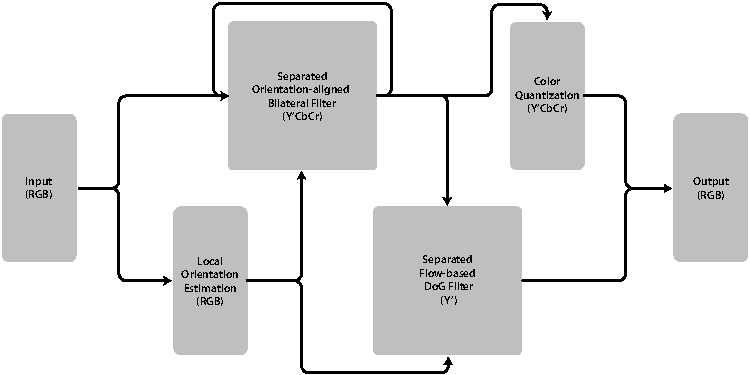
\includegraphics[width=\textwidth]{graphics/test3}
    \caption{Stet clita kasd gubergren, no sea takimata sanctus est Lorem ipsum dolor sit amet. Lorem ipsum dolor sit amet, consetetur sadipscing elitr.}
\end{figure}

Consetetur sadipscing elitr, \citep{Yang.etal-1996} sed diam nonumy eirmod tempor invidunt ut labore et dolore magna aliquyam erat, sed diam voluptua. At vero eos et accusam et justo duo dolores et ea rebum. Stet clita kasd gubergren, no sea takimata sanctus est Lorem ipsum dolor sit amet. Lorem ipsum dolor sit amet, consetetur sadipscing elitr, sed diam nonumy eirmod tempor invidunt ut labore et dolore magna aliquyam erat, sed diam voluptua. At vero eos et accusam et justo duo dolores et ea rebum. Stet clita kasd gubergren, no sea takimata sanctus est Lorem ipsum dolor sit amet. Lorem ipsum dolor sit amet, consetetur sadipscing elitr, sed diam nonumy eirmod tempor invidunt ut labore et dolore magna aliquyam erat, sed diam voluptua. At vero eos et accusam et justo duo dolores et ea rebum. Stet clita kasd gubergren, no sea takimata sanctus.   


\subsection{At vero eos et accusam}
Lorem ipsum dolor sit amet, consetetur sadipscing elitr, sed diam nonumy eirmod tempor invidunt ut labore et dolore magna aliquyam erat, sed diam voluptua. At vero eos et accusam et justo duo dolores et ea rebum. Stet clita kasd gubergren, no sea takimata sanctus est Lorem ipsum dolor sit amet. Lorem ipsum dolor sit amet, consetetur sadipscing elitr, sed diam nonumy eirmod tempor invidunt ut labore et dolore magna aliquyam erat, sed diam voluptua. At vero eos et accusam et justo duo dolores et ea rebum. Stet clita kasd gubergren, no sea takimata sanctus est Lorem ipsum dolor sit amet. Lorem ipsum dolor sit amet, consetetur sadipscing elitr, sed diam nonumy eirmod tempor invidunt ut labore et dolore magna aliquyam erat, sed diam voluptua. At vero eos et accusam et justo duo dolores et ea rebum. Stet clita kasd gubergren, no sea takimata sanctus est Lorem ipsum dolor sit amet.   
Duis autem vel eum iriure dolor in hendrerit in vulputate velit esse molestie consequat, vel illum dolore eu feugiat nulla facilisis at vero eros et accumsan et iusto odio dignissim qui blandit praesent luptatum zzril delenit augue duis dolore te feugait nulla facilisi. Lorem ipsum dolor sit amet, consectetuer adipiscing elit, sed diam nonummy nibh euismod tincidunt ut laoreet dolore magna aliquam erat volutpat.   

Ut wisi enim ad minim veniam, quis nostrud exerci tation ullamcorper suscipit lobortis nisl ut aliquip ex ea commodo consequat. Duis autem vel eum iriure dolor in hendrerit in vulputate velit esse molestie consequat, vel illum dolore eu feugiat \citep{Guichard.Morel-2003} nulla facilisis at vero eros et accumsan et iusto odio dignissim qui blandit praesent luptatum zzril delenit augue duis dolore te feugait nulla facilisi.   
Nam liber tempor cum soluta nobis eleifend option congue nihil imperdiet doming id quod mazim placerat facer possim assum. Lorem ipsum dolor sit amet, consectetuer adipiscing elit, sed diam nonummy nibh euismod tincidunt ut laoreet dolore magna aliquam erat volutpat. Ut wisi enim ad minim veniam, quis nostrud exerci tation ullamcorper suscipit lobortis nisl ut aliquip ex ea commodo consequat.   
Duis autem vel eum iriure dolor in hendrerit in vulputate velit esse molestie consequat, vel illum dolore eu feugiat nulla facilisis.   

\begin{figure}
    \centering%
    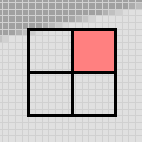
\includegraphics[width=0.32\textwidth]{graphics/test0}
    \caption{Stet clita kasd gubergren, no sea takimata sanctus est.}
\end{figure}


\section{At accusam aliquyam}
At vero eos et accusam et justo duo dolores et ea rebum. Stet clita kasd gubergren, no sea takimata sanctus est Lorem ipsum dolor sit amet. Lorem ipsum dolor sit amet, consetetur sadipscing elitr, sed diam nonumy eirmod tempor invidunt ut labore et dolore magna aliquyam erat, sed diam voluptua. At vero eos et accusam et justo duo dolores et ea rebum. Stet clita kasd gubergren, no sea takimata sanctus est Lorem ipsum dolor sit amet. Lorem ipsum dolor sit amet, consetetur sadipscing elitr, At accusam aliquyam diam diam dolore dolores duo eirmod eos erat, et nonumy sed tempor et et invidunt justo labore Stet clita ea et gubergren, kasd magna no rebum. sanctus sea sed takimata ut vero voluptua. est Lorem ipsum dolor sit amet. Lorem ipsum dolor sit amet, consetetur sadipscing elitr, sed diam nonumy eirmod tempor invidunt ut labore et dolore magna aliquyam erat.   
\begin{itemize}
\item Duis autem vel eum iriure dolor in hendrerit in vulputate velit esse molestie consequat, vel illum dolore eu feugiat nulla facilisis at vero eros et
\item Et iusto odio dignissim qui blandit praesent luptatum zzril delenit augue duis dolore te feugait nulla facilisi. Lorem ipsum dolor sit.
\item Amet, consectetuer adipiscing elit, sed diam nonummy nibh euismod tincidunt ut laoreet dolore magna aliquam erat volutpat.   
\end{itemize}

Consetetur sadipscing elitr, \citep{Barash.Comaniciu-2004} sed diam nonumy eirmod tempor invidunt ut labore et dolore magna aliquyam erat, sed diam voluptua. At vero eos et accusam et justo duo dolores et ea rebum. Stet clita kasd gubergren, no sea takimata sanctus est Lorem ipsum dolor sit amet. Lorem ipsum dolor sit amet, consetetur sadipscing elitr, sed diam nonumy eirmod tempor invidunt ut labore et dolore magna aliquyam erat, sed diam voluptua. At vero eos et accusam et justo duo dolores et ea rebum. Stet clita kasd gubergren, no sea takimata sanctus est Lorem ipsum dolor sit amet. Lorem ipsum dolor sit amet, consetetur sadipscing elitr, sed diam nonumy eirmod tempor invidunt ut labore et dolore magna aliquyam erat, sed diam voluptua. At vero eos et accusam et justo duo dolores et ea rebum. Stet clita kasd gubergren, no sea takimata sanctus.   
Lorem ipsum dolor sit amet, consetetur sadipscing elitr, sed diam nonumy eirmod tempor invidunt ut labore et dolore magna aliquyam erat, sed diam voluptua. At vero eos et accusam et justo duo dolores et ea rebum. Stet clita kasd gubergren, no sea takimata sanctus est Lorem ipsum dolor sit amet. Lorem ipsum dolor sit amet, consetetur sadipscing elitr, sed diam nonumy eirmod tempor invidunt ut labore et dolore magna aliquyam erat, sed diam voluptua. At vero eos et accusam et justo duo dolores et ea rebum. Stet clita kasd gubergren, no sea takimata sanctus est Lorem ipsum dolor sit amet. Lorem ipsum dolor sit amet, consetetur sadipscing elitr, sed diam nonumy eirmod tempor invidunt ut labore et dolore magna aliquyam erat, sed diam voluptua. At vero eos et accusam et justo duo dolores et ea rebum. Stet clita kasd gubergren, no sea takimata sanctus est Lorem ipsum dolor sit amet.   
Duis autem vel eum iriure dolor in hendrerit in vulputate velit esse molestie consequat, vel illum dolore eu feugiat nulla facilisis at vero eros et accumsan et iusto odio dignissim qui blandit praesent luptatum zzril delenit augue duis dolore te feugait nulla facilisi. Lorem ipsum dolor sit amet, consectetuer adipiscing elit, sed diam nonummy nibh euismod tincidunt ut laoreet dolore magna aliquam erat volutpat.   

\begin{figure}
    \subcaptionbox{\label{fig:test3a}Test 1}{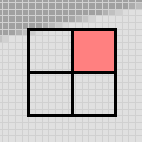
\includegraphics[width=0.32\textwidth]{graphics/test0}}%
    \hfill%
    \subcaptionbox{\label{fig:test3b}Test 2}{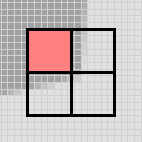
\includegraphics[width=0.32\textwidth]{graphics/test1}}%
    \hfill%
    \subcaptionbox{\label{fig:test3c}Test 3}{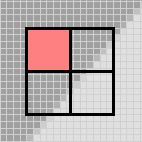
\includegraphics[width=0.32\textwidth]{graphics/test2}}%
    \caption{Stet clita kasd gubergren, no sea takimata}
    \label{fig:test3}
\end{figure}

\textbf{Ut wisi enim} ad minim veniam, quis nostrud exerci tation ullamcorper suscipit lobortis nisl ut aliquip ex ea commodo consequat. Duis autem vel eum iriure dolor in hendrerit in vulputate velit esse molestie consequat, vel illum dolore eu feugiat nulla facilisis at vero eros et accumsan et iusto odio dignissim qui blandit praesent luptatum zzril delenit augue duis dolore te feugait nulla facilisi.   
Nam liber tempor cum soluta nobis eleifend option congue nihil imperdiet doming id quod mazim placerat facer possim assum. Lorem ipsum dolor sit amet, consectetuer adipiscing elit, sed diam nonummy nibh euismod tincidunt ut laoreet dolore magna aliquam erat volutpat. Ut wisi enim ad minim veniam, quis nostrud exerci tation ullamcorper suscipit lobortis nisl ut aliquip ex ea commodo consequat.   
Duis autem vel eum iriure dolor in hendrerit in vulputate velit esse molestie consequat, vel illum dolore eu feugiat nulla facilisis.   

At vero eos et accusam et \citep{Black.Rangarajan-1996} justo duo dolores et ea rebum. Stet clita kasd gubergren, no sea takimata sanctus est Lorem ipsum dolor sit amet. Lorem ipsum dolor sit amet, consetetur sadipscing elitr, sed diam nonumy eirmod tempor invidunt ut labore et dolore magna aliquyam erat, sed diam voluptua. At vero eos et accusam et justo duo dolores et ea rebum. Stet clita kasd gubergren, no sea takimata sanctus est Lorem ipsum dolor sit amet. Lorem ipsum dolor sit amet, consetetur sadipscing elitr, At accusam aliquyam diam diam dolore dolores duo eirmod eos erat, et nonumy sed tempor et et invidunt justo labore Stet clita ea et gubergren, kasd magna no rebum. sanctus sea sed takimata ut vero voluptua. est Lorem ipsum dolor sit amet. Lorem ipsum dolor sit amet, consetetur sadipscing elitr, sed diam nonumy eirmod tempor invidunt ut labore et dolore magna aliquyam erat.   

Referenzieren von Abbildungen: Abbildunng~\ref{fig:test3}, Abbildung~\ref{fig:test3a}, Abbildung~\ref{fig:test3}\subref{fig:test3a}-\subref{fig:test3c}.

Consetetur sadipscing elitr, sed diam nonumy eirmod tempor invidunt ut labore et dolore magna aliquyam erat, sed diam voluptua. At vero eos et accusam et justo duo dolores et ea rebum. Stet clita kasd gubergren, no sea takimata sanctus est Lorem ipsum dolor sit amet. Lorem ipsum dolor sit amet, consetetur sadipscing elitr, sed diam nonumy eirmod tempor invidunt ut labore et dolore magna aliquyam erat, sed diam voluptua. At vero eos et accusam et justo duo dolores et ea rebum. Stet clita kasd gubergren, no sea takimata sanctus est Lorem ipsum dolor sit amet. Lorem ipsum dolor sit amet, consetetur sadipscing elitr, sed diam nonumy eirmod tempor invidunt ut labore et dolore magna aliquyam erat, sed diam voluptua. At vero eos et accusam et justo duo dolores et ea rebum. Stet clita kasd gubergren, no sea takimata sanctus.   

Lorem ipsum dolor sit amet, consetetur sadipscing elitr, sed diam nonumy eirmod tempor invidunt ut labore et dolore magna aliquyam erat, sed diam voluptua. At vero eos et accusam et justo duo dolores et ea rebum. Stet clita kasd gubergren, no sea takimata sanctus est Lorem ipsum dolor sit amet. Lorem ipsum dolor sit amet, consetetur sadipscing elitr, sed diam nonumy eirmod tempor invidunt ut labore et dolore magna aliquyam erat, sed diam voluptua. At vero eos et accusam et justo duo dolores et ea rebum. Stet clita kasd gubergren, no sea takimata sanctus est Lorem ipsum dolor sit amet. Lorem ipsum dolor sit amet, consetetur sadipscing elitr, sed diam nonumy eirmod tempor invidunt ut labore et dolore magna aliquyam erat, sed diam voluptua. At vero eos et accusam et justo duo dolores et ea rebum. Stet clita kasd gubergren, no sea takimata sanctus est Lorem ipsum dolor sit amet.   
Duis autem vel eum iriure dolor in hendrerit in vulputate velit esse molestie consequat, vel illum dolore eu feugiat nulla facilisis at vero eros et accumsan et iusto odio dignissim qui blandit praesent luptatum zzril delenit augue duis dolore te feugait nulla facilisi. Lorem ipsum dolor sit amet, consectetuer adipiscing elit, sed diam nonummy nibh euismod tincidunt ut laoreet dolore magna aliquam erat volutpat.   
Ut wisi enim ad minim veniam, quis nostrud exerci tation ullamcorper suscipit lobortis nisl ut aliquip ex ea commodo consequat. Duis autem vel eum iriure dolor in hendrerit in vulputate velit esse molestie consequat, vel illum dolore eu feugiat nulla facilisis at vero eros et accumsan et iusto odio dignissim qui blandit praesent luptatum zzril delenit augue duis dolore te feugait nulla facilisi.   
Nam liber tempor cum soluta nobis eleifend option congue nihil imperdiet doming id quod mazim placerat facer possim assum. Lorem ipsum dolor sit amet, consectetuer adipiscing elit, sed diam nonummy nibh euismod tincidunt ut laoreet dolore magna aliquam erat volutpat. Ut wisi enim ad minim veniam, quis nostrud exerci tation ullamcorper suscipit lobortis nisl ut aliquip ex ea commodo consequat.   
Duis autem vel eum iriure dolor in hendrerit in vulputate velit esse molestie consequat, vel illum dolore eu feugiat nulla facilisis.   

\lstinputlisting[float,caption={Consetetur sadipscing elitr, sed diam nonumy eirmod tempor invidunt ut labore et dolore magna.}]{graphics/bf.glsl}%

At vero eos et accusam et justo duo dolores et ea rebum. Stet clita kasd gubergren, no sea takimata sanctus est Lorem ipsum dolor sit amet. Lorem ipsum dolor sit amet, consetetur sadipscing elitr, sed diam nonumy eirmod tempor invidunt ut labore et dolore magna aliquyam erat, sed diam voluptua. At vero eos et accusam et justo duo dolores et ea rebum. Stet clita kasd gubergren, no sea takimata sanctus est Lorem ipsum dolor sit amet. Lorem ipsum dolor sit amet, consetetur sadipscing elitr, At accusam aliquyam diam diam dolore dolores duo eirmod eos erat, et nonumy sed tempor et et invidunt justo labore Stet clita ea et gubergren, kasd magna no rebum. sanctus sea sed takimata ut vero voluptua. est Lorem ipsum dolor sit amet. Lorem ipsum dolor sit amet, consetetur sadipscing elitr, sed diam nonumy eirmod tempor invidunt ut labore et dolore magna aliquyam erat.   

Consetetur sadipscing elitr, sed diam nonumy eirmod tempor invidunt ut labore et dolore magna aliquyam erat, sed diam voluptua. At vero eos et accusam et justo duo dolores et ea rebum. Stet clita kasd gubergren, no sea takimata sanctus est Lorem ipsum dolor sit amet. Lorem ipsum dolor sit amet, consetetur sadipscing elitr, sed diam nonumy eirmod tempor invidunt ut labore et dolore magna aliquyam erat, sed diam voluptua. At vero eos et accusam et justo duo dolores et ea rebum. Stet clita kasd gubergren, no sea takimata sanctus est Lorem ipsum dolor sit amet. Lorem ipsum dolor sit amet, consetetur sadipscing elitr, sed diam nonumy eirmod tempor invidunt ut labore et dolore magna aliquyam erat, sed diam voluptua. At vero eos et accusam et justo duo dolores et ea rebum. Stet clita kasd gubergren, no sea takimata sanctus.   

Lorem ipsum dolor sit amet, consetetur sadipscing elitr, sed diam nonumy eirmod tempor invidunt ut labore et dolore magna aliquyam erat, sed diam voluptua. At vero eos et accusam et justo duo dolores et ea rebum. Stet clita kasd gubergren, no sea takimata sanctus est Lorem ipsum dolor sit amet. Lorem ipsum dolor sit amet, consetetur sadipscing elitr, sed diam nonumy eirmod tempor invidunt ut labore et dolore magna aliquyam erat, sed diam voluptua. At vero eos et accusam et justo duo dolores et ea rebum. Stet clita kasd gubergren, no sea takimata sanctus est Lorem ipsum dolor sit amet. Lorem ipsum dolor sit amet, consetetur sadipscing elitr, sed diam nonumy eirmod tempor invidunt ut labore et dolore magna aliquyam erat, sed diam voluptua. At vero eos et accusam et justo duo dolores et ea rebum. Stet clita kasd gubergren, no sea takimata sanctus est Lorem ipsum dolor sit amet.   
Duis autem vel eum iriure dolor in hendrerit in vulputate velit esse molestie consequat, vel illum dolore eu feugiat nulla facilisis at vero eros et accumsan et iusto odio dignissim qui blandit praesent luptatum zzril delenit augue duis dolore te feugait nulla facilisi. Lorem ipsum dolor sit amet, consectetuer adipiscing elit, sed diam nonummy nibh euismod tincidunt ut laoreet dolore magna aliquam erat volutpat.   

\begin{figure}
    \subcaptionbox{Test 1}{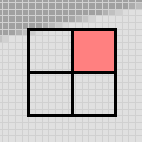
\includegraphics[width=0.32\textwidth]{graphics/test0}}%
    \hfill%
    \subcaptionbox{Test 2}{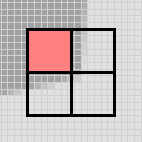
\includegraphics[width=0.32\textwidth]{graphics/test1}}%
    \hfill%
    \subcaptionbox{Test 3}{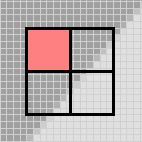
\includegraphics[width=0.32\textwidth]{graphics/test2}}%
    \par\medskip%
    \subcaptionbox{Test 1}{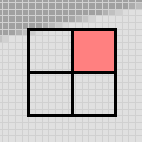
\includegraphics[width=0.32\textwidth]{graphics/test0}}%
    \hfill%
    \subcaptionbox{Test 2}{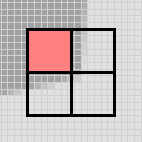
\includegraphics[width=0.32\textwidth]{graphics/test1}}%
    \hfill%
    \subcaptionbox{Test 3}{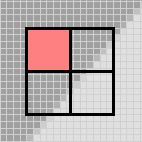
\includegraphics[width=0.32\textwidth]{graphics/test2}}%
    \caption{Stet clita kasd gubergren, no sea takimata sanctus est. Stet clita kasd gubergren, no sea takimata sanctus est.}
\end{figure}

Ut wisi enim ad minim veniam, quis nostrud exerci tation ullamcorper suscipit lobortis nisl ut aliquip ex ea commodo consequat. Duis autem vel eum iriure dolor in hendrerit in vulputate velit esse molestie consequat, vel illum dolore eu feugiat nulla facilisis at vero eros et accumsan et iusto odio dignissim qui blandit praesent luptatum zzril delenit augue duis dolore te feugait nulla facilisi.   
Nam liber tempor cum soluta nobis eleifend option congue nihil imperdiet doming id quod mazim placerat facer possim assum. Lorem ipsum dolor sit amet, consectetuer adipiscing elit, sed diam nonummy nibh euismod tincidunt ut laoreet dolore magna aliquam erat volutpat. Ut wisi enim ad minim veniam, quis nostrud exerci tation ullamcorper suscipit lobortis nisl ut aliquip ex ea commodo consequat.   
Duis autem vel eum iriure dolor in hendrerit in vulputate velit esse molestie consequat, vel illum dolore eu feugiat nulla facilisis.   

At vero eos et accusam et justo duo dolores et ea rebum. Stet clita kasd gubergren, no sea takimata sanctus est Lorem ipsum dolor sit amet. Lorem ipsum dolor sit amet, consetetur sadipscing elitr, sed diam nonumy eirmod tempor invidunt ut labore et dolore magna aliquyam erat, sed diam voluptua. At vero eos et accusam et justo duo dolores et ea rebum. Stet clita kasd gubergren, no sea takimata sanctus est Lorem ipsum dolor sit amet. Lorem ipsum dolor sit amet, consetetur sadipscing elitr, At accusam aliquyam diam diam dolore dolores duo eirmod eos erat, et nonumy sed tempor et et invidunt justo labore Stet clita ea et gubergren, kasd magna no rebum. sanctus sea sed takimata ut vero voluptua. est Lorem ipsum dolor sit amet. Lorem ipsum dolor sit amet, consetetur sadipscing elitr, sed diam nonumy eirmod tempor invidunt ut labore et dolore magna aliquyam erat.   
Consetetur sadipscing elitr, sed diam nonumy eirmod tempor invidunt ut labore et dolore magna aliquyam erat, sed diam voluptua. At vero eos et accusam et justo duo dolores et ea rebum. Stet clita kasd gubergren, no sea takimata sanctus est Lorem ipsum dolor sit amet. Lorem ipsum dolor sit amet, consetetur sadipscing elitr, sed diam nonumy eirmod tempor invidunt ut labore et dolore magna aliquyam erat, sed diam voluptua. At vero eos et accusam et justo duo dolores et ea rebum. Stet clita kasd gubergren, no sea takimata sanctus est Lorem ipsum dolor sit amet. Lorem ipsum dolor sit amet, consetetur sadipscing elitr, sed diam nonumy eirmod tempor invidunt ut labore et dolore magna aliquyam erat, sed diam voluptua. At vero eos et accusam et justo duo dolores et ea rebum. Stet clita kasd gubergren, no sea takimata sanctus.   
Lorem ipsum dolor sit amet, consetetur sadipscing elitr, sed diam nonumy eirmod tempor invidunt ut labore et dolore magna aliquyam erat, sed diam voluptua. At vero eos et accusam et justo duo dolores et ea rebum. Stet clita kasd gubergren, no sea takimata sanctus est Lorem ipsum dolor sit amet. Lorem ipsum
% % !TeX root = foo-thesis.tex

\chapter{Sample File from SIAM \LaTeX\ Book Macro Package}

%\begin{chapterquote}[120pt]
%We have nothing to fear but fear itself.\\
%---{\upshape Franklin D. Roosevelt}\\[6pt]
%I am not a crook.\\
%---{\upshape Richard M. Nixon}
%\end{chapterquote}

\newtheorem{theorem}{Theorem}
\newtheorem{lemma}{Lemma}
\newtheorem{proposition}{Proposition}
\newtheorem{corollary}{Corollary}
\newtheorem{definition}{Definition}

\newcommand{\pe}{\psi}
\def\d{\delta} 
\def\ds{\displaystyle} 
\def\e{{\epsilon}} 
\def\eb{\bar{\eta}}  
\def\enorm#1{\|#1\|_2} 
\def\Fp{F^\prime}  
\def\fishpack{{FISHPACK}} 
\def\fortran{{FORTRAN}} 
\def\gmres{{GMRES}} 
\def\gmresm{{\rm GMRES($m$)}} 
\def\Kc{{\cal K}} 
\def\norm#1{\|#1\|} 
\def\wb{{\bar w}} 
\def\zb{{\bar z}} 
\def\bfE{\mbox{\boldmath$E$}}
\def\bfG{\mbox{\boldmath$G$}}


\section{Introduction and Examples}
This paper presents a sample file for the use of SIAM's
\LaTeX\ macro package. It illustrates the features\index{Features} of the%
\footnote{This is a sample footnote. This is a sample footnote. 
This is a sample footnote. This is a sample footnote. 
This is a sample footnote. This is a sample footnote.}
macro package, using actual examples culled from various
papers published in SIAM's journals. It is to be expected
that this sample will provide examples of how to use the
macros to generate standard elements of journal papers,
e.g., theorems, definitions, or figures. This paper also
serves as an example of SIAM's stylistic preferences for
the formatting of such elements as bibliographic references,
displayed equations, and equation arrays, among others.
Some special circumstances are not dealt with in this
sample file; for such information one should see the
included documentation file.

{\em Note:} This paper is not to be read in any form for content. 
The conglomeration of equations, lemmas, and other text elements were 
put together solely for typographic illustrative purposes and don't 
make any sense as lemmas, equations, etc.

\subsection{Sample text}\index{Sample text}
Let $S=[s_{ij}]$ ($1\leq i,j\leq n$) be a $(0,1,-1)$-matrix
of order $n$. Then $S$ is a {\em sign-nonsingular matrix}
(SNS-matrix) provided that each real matrix with the same
sign pattern as $S$ is nonsingular. There has been
considerable recent interest in constructing and
characterizing SNS-matrices \cite{Healey.etal-2004}, \cite{Dai.etal-2007}. There
has also been interest in strong forms of
sign-nonsingularity \cite{Balikai.etal-2008}. In this paper we give a new
generalization of SNS-matrices and investigate some of
their basic properties.


Let $S=[s_{ij}]$ be a $(0,1,-1)$-matrix of order $n$ and
let $C=[c_{ij}]$ be a real matrix of order $n$. The pair
$(S,C)$ is called a {\em matrix pair of order} $n$.
Throughout, $X=[x_{ij}]$ denotes a matrix of order $n$
whose entries are algebraically independent indeterminates
over the real field. Let $S\circ X$ denote the Hadamard
product (entrywise product) of $S$ and $X$. We say that the
pair $(S,C)$ is a {\em sign-nonsingular matrix pair of
order} $n$, abbreviated SNS-{\em matrix pair of order} $n$,
provided that the matrix \[A=S\circ X+C\] is nonsingular
for all positive real values of the $x_{ij}$.  If $C=O$
then the pair $(S,O)$ is a SNS-matrix pair if and only if
$S$ is a SNS-matrix.  If $S=O$ then the pair $(O,C)$ is a
SNS-matrix pair if and only if $C$ is nonsingular. Thus
SNS-matrix pairs include both nonsingular matrices and
sign-nonsingular matrices as special cases.

The pairs $(S,C)$ with
\[S=\left[\begin{array}{cc}1&0\\0&0\end{array}\right],\qquad 
C=\left[\begin{array}{cc}1&1\\1&1\end{array}\right]\] and 
\[S=\left[\begin{array}{ccc}1&1&0\\1&1&0\\0&0&0\end{array}\right],\qquad 
C=\left[\begin{array}{ccc}0&0&1\\0&2&0\\
3&0&0\end{array}\right]\] are examples of SNS-matrix pairs.

\subsection{Some list environments}
In this paper we consider the evaluation of integrals of the 
following forms:
\begin{equation}
\int_a^b \left( \sum_i E_i B_{i,k,x}(t) \right)
         \left( \sum_j F_j B_{j,l,y}(t) \right) dt,\label{problem}
\end{equation}
\begin{equation}
\int_a^b f(t) \left( \sum_i E_i B_{i,k,x}(t) \right) dt,\label{problem2}
\end{equation}
where $B_{i,k,x}$ is the $i$th B-spline of order $k$ defined over the
knots $x_i, x_{i+1}, \ldots, x_{i+k}$.
We will consider B-splines normalized so that their integral is one.
The splines may be of different orders and
defined on different knot sequences $x$ and $y$.
Often the limits of integration will be the entire real line, $-\infty$
to $+\infty$. Note that (\ref{problem}) is a special case of (\ref{problem2})
where $f(t)$ is a spline.


There are five different methods for calculating (\ref{problem})
that will be considered; here is the \verb+remunerate+ list:
\begin{enumerate}
\item Use Gauss quadrature on each interval.
\item Convert the integral to a linear combination of
      integrals of products of B-splines and provide a recurrence for
      integrating the product of a pair of B-splines.
\item Convert the sums of B-splines to piecewise
      B\'{e}zier format and integrate segment
      by segment using the properties of the Bernstein polynomials.
\item Express the product of a pair of B-splines as a linear combination
      of B-splines.
      Use this to reformulate the integrand as a linear combination
      of B-splines, and integrate term by term.
\item Integrate by parts.
\end{enumerate}
Of these five, only methods 1 and 5 are suitable for calculating 
(\ref{problem2}). The first four methods will be touched on and the 
last will be discussed at length.

Here is the bullet list:
\begin{itemize}
\item Use Gauss quadrature on each interval.
\item Convert the integral to a linear combination of
      integrals of products of B-splines and provide a recurrence for
      integrating the product of a pair of B-splines.
\item Convert the sums of B-splines to piecewise
      B\'{e}zier format and integrate segment
      by segment using the properties of the Bernstein polynomials.
\item Express the product of a pair of B-splines as a linear combination
      of B-splines.
      Use this to reformulate the integrand as a linear combination
      of B-splines, and integrate term by term.
\item Integrate by parts.
\end{itemize}
and, finally, the \verb+romannum+ list:
\begin{enumerate}
\item Use Gauss quadrature on each interval.
\item Convert the integral to a linear combination of
      integrals of products of B-splines and provide a recurrence for
      integrating the product of a pair of B-splines.
\item Convert the sums of B-splines to piecewise
      B\'{e}zier format and integrate segment
      by segment using the properties of the Bernstein polynomials.
\item Express the product of a pair of B-splines as a linear combination
      of B-splines.
      Use this to reformulate the integrand as a linear combination
      of B-splines, and integrate term by term.
\item Integrate by parts.
\end{enumerate}

%\subsection{An algorithm}
%Here is a sample algorithm:
%\begin{algorithm}{The Sample Algorithm}
%For $i=1$ to 10\\
%print ``Hello world''\\
%end
%\end{algorithm}
%Some text after the algorithm. Some text after the algorithm. Some text after the algorithm. 
%Some text after the algorithm. Some text after the algorithm. 

\subsection{Some displayed equations}
     By introducing the product topology on  $\mathbb{R}^{m \times m} \times
\mathbb{R}^{n \times n}$  with the induced inner product
\begin{equation}
\langle (A_{1},B_{1}), (A_{2},B_{2})\rangle := \langle A_{1},A_{2}\rangle 
+ \langle B_{1},B_{2}\rangle,\label{eq2.10}
\end{equation}
we calculate the Fr\'{e}chet derivative of  $F$  as follows:
\begin{align}
 F'(U,V)(H,K) &= \langle R(U,V),H\Sigma V^{T} + U\Sigma K^{T} -
P(H\Sigma V^{T} + U\Sigma K^{T})\rangle \nonumber \\
         &= \langle R(U,V),H\Sigma V^{T} + U\Sigma K^{T}\rangle \label{eq2.11} \\
&= \langle R(U,V)V\Sigma^{T},H\rangle + \langle \Sigma^{T}U^{T}R(U,V),K^{T}\rangle.     \nonumber
\end{align}
In the middle line of (\ref{eq2.11}) we have used the fact that the range of
$R$ is always perpendicular to the range of $P$.  The gradient $\nabla F$  of
$F$, therefore,  may be interpreted as the
pair of matrices:
\begin{equation}
 \nabla F(U,V) = (R(U,V)V\Sigma^{T},R(U,V)^{T}U\Sigma ) \in
R^{m \times m} \times R^{n \times n}.       			\label{eq2.12}
\end{equation}
Because of the product topology, we know
\begin{equation}
 {\cal T}_{(U,V)}({\cal O} (m) \times {\cal O} (n)) =
{\cal T}_{U}{\cal O} (m) \times {\cal T}_{V}{\cal O} (n),  		\label{eq2.13}
\end{equation}
where  ${\cal T}_{(U,V)}({\cal O} (m) \times {\cal O} (n))$  stands for the
tangent space to the manifold  ${\cal O} (m) \times {\cal O} (n)$  at  $(U,V)
\in {\cal O} (m) \times {\cal O} (n)$  and so on.  The projection of
$\nabla F(U,V)$  onto  ${\cal T}_{(U,V)}({\cal O} (m) \times {\cal O} (n))$,
therefore, is the product of the projection of the first component of
$\nabla F(U,V)$  onto  ${\cal T}_{U}{\cal O} (m)$  and the projection of the
second component of  $\nabla F(U,V)$  onto  ${\cal T}_{V}{\cal O} (n)$. 
In particular, we claim that the
projection $ g(U,V)$  of the gradient  $\nabla F(U,V)$  onto
${\cal T}_{(U,V)}({\cal O} (m) \times {\cal O} (n))$  is given by the pair of
matrices:
\begin{align}
g(U,V) =& \left( \frac{R(U,V)V\Sigma^{T}U^{T}-U\Sigma V^{T}R(U,V)^{T}}{2}U,
\right.			\nonumber \\[-1.5ex]
\label{eq2.14}\\[-1.5ex]
&\quad\!\left. \frac{R(U,V)^{T}U\Sigma V^{T}-V
   \Sigma^{T}U^{T}R(U,V)}{2}V \right).\nonumber
\end{align}
Thus, the vector field
\begin{equation}
\frac{d(U,V)}{dt} = -g(U,V) 	\label{eq2.15}
\end{equation}
defines a steepest descent flow on the manifold  ${\cal O} (m) \times
{\cal O} (n)$ for the objective function  $F(U,V)$.

\section{Main Results}

Let $(S,C)$ be a matrix pair of order $n$.  The determinant
\[\det (S\circ X+C)\] 
is a polynomial in the indeterminates of $X$ of degree at
most $n$ over the real field. We call this polynomial the
{\em indicator polynomial} of the matrix pair $(S,C)$
because of the following proposition.

\begin{theorem} 
\label{th:prop} 
The matrix pair $(S,C)$ is a {\rm SNS}-matrix pair if and
only if all the nonzero coefficients in its indicator
polynomial have the same sign and there is at least one
nonzero coefficient.
\end{theorem}

\begin{proof}
Assume that $(S,C)$ is a SNS-matrix pair.  Clearly the
indicator polynomial has a nonzero coefficient.  Consider a
monomial
\begin{equation} 
\label{eq:mono} 
b_{i_{1},\ldots,i_{k};j_{1},\ldots,j_{k}}x_{i_{1}j_{1}}\cdots
x_{i_{k}j_{k}}
\end{equation} 
occurring in the indicator polynomial with a nonzero
coefficient.  By taking the $x_{ij}$ that occur in
(\ref{eq:mono}) large and all others small, we see that any
monomial that occurs in the indicator polynomial with a
nonzero coefficient can be made to dominate all others.
Hence all the nonzero coefficients have the same sign. The
converse is immediate. \qquad\end{proof}


For SNS-matrix pairs $(S,C)$ with $C=O$ the indicator
polynomial is a homogeneous polynomial of degree $n$. In
this case Theorem \ref{th:prop} is a standard fact about
SNS-matrices.

\begin{lemma}[Stability]
\label{stability}
Given $T>0$, suppose that $\| \epsilon (t) \|_{1,2} \leq h^{q-2}$
for $0 \leq t \leq T$ and $q \geq 6$. 
Then there exists a positive number $B$ that depends on
$T$ and the exact solution $\pe$ only such that for all $0 \leq t \leq T$,
\begin{equation}
\label{Gron}
\frac {d}{dt} \| \epsilon (t) \| _{1,2}  \leq B
   ( h^{q-3/2} + \| \epsilon (t) \|_{1,2})\;.
\end{equation}
The function $B(T)$ can be chosen to be nondecreasing in time.
\end{lemma}

\begin{theorem} 
\label{th:gibson} 
The maximum number of nonzero entries in a {\rm SNS}-matrix
$S$ of order $n$ equals \[\frac{n^{2}+3n-2}{2}\] with
equality if and only if there exist permutation matrices
such that $P|S|Q=T_{n}$ where
\begin{equation} 
\label{eq:gibson} 
T_{n}=\left[\begin{array}{cccccc} 1&1&\cdots&1&1&1\\
1&1&\cdots&1&1&1\\ 0&1&\cdots&1&1&1\\ 
\vdots&\vdots&\ddots&\vdots&\vdots&\vdots\\ 
0&0&\cdots&1&1&1\\ 0&0&\cdots&0&1&1\end{array}\right]. 
\end{equation} 
\end{theorem}

We note for later use that each submatrix of $T_{n}$ of
order $n-1$ has all 1s on its main diagonal.

We now obtain a bound on the number of nonzero entries of
$S$ in a SNS-matrix pair $(S,C)$ in terms of the degree of
the indicator polynomial. We denote the strictly upper
triangular (0,1)-matrix of order $m$ with all 1s above the
main diagonal by $U_{m}$. The all 1s matrix of size $m$ by
$p$ is denoted by $J_{m,p}$.

\begin{proposition}[Convolution theorem]
\label{pro:2.1}  Let
\begin{eqnarray*}
a\ast u(t) = \int_0^t a(t- \tau) u(\tau) d\tau, \hspace{.2in} t \in
(0, \infty).
\end{eqnarray*}
Then
\begin{eqnarray*}
\widehat{a\ast u}(s) = \widehat{a}(s)\widehat{u}(s).
\end{eqnarray*}
\end{proposition}

\begin{lemma}
\label{lem:3.1}
For $s_0 >0$, if
$$
\int_0^{\infty} e^{-2s_0 t}v^{(1)}(t) v(t) dt \; \leq 0 \;,
$$
then
\begin{eqnarray*}
\int_0^{\infty} e^{-2s_0 t} v^2(t) dt \; \leq \; \frac{1}{2s_0} v^2(0).
\end{eqnarray*}
\end{lemma}

\noindent{\em Proof.}
Applying integration by parts, we obtain
\begin{eqnarray*}
\int_0^{\infty} e^{-2s_0 t} [v^2(t)-v^2(0)] dt
&=&\lim_{t\rightarrow \infty}\left (
-\frac{1}{2s_0}e^{-2s_0 t}v^2(t) \right ) +\frac{1}{s_0}
\int_0^{\infty} e^{-2s_0 t}v^{(1)}(t)v(t)dt\\
&\leq& \frac{1}{s_0} \int_0^{\infty} e^{-2s_0 t} v^{(1)}(t)v(t) dt \;\;
\leq \;\; 0.
\end{eqnarray*}

\begin{corollary}\label{c4.1}
Let $ \bfE $ satisfy $(5)$--$(6)$ and
suppose $ \bfE^h $ satisfies $(7)$ and $(8)$
with a general $ \bfG $.  Let $ \bfG= \nabla \times {\bf \Phi} + \nabla p,$
$p \in H_0^1 (\Omega) $. Suppose that $\nabla p$ and $ \nabla \times 
{\bf \Phi} $ satisfy all the assumptions of Theorems $4.1$ and  
$4.2$, respectively. In addition suppose all the regularity
assumptions of Theorems $4.1$--$4.2$ are satisfied.  Then 
for $ 0 \le t \le T $ and $ 0 < \epsilon \le \epsilon_0 $ there exists a 
constant $ C = C(\epsilon, T) $ such that
$$
\Vert (\bfE - \bfE^h)(t) \Vert_0 \le C h^{k+1- \epsilon},
$$
where $ C $ also depends on the constants given in Theorems 
$4.1$ and $4.2$.
\end{corollary}


\begin{definition}
Let $S$ be an isolated invariant set with isolating neighborhood $N$.
An {\em index pair} for $S$ is a pair of compact sets $(N_{1},N_{0})$
with $N_{0} \subset N_{1} \subset N$ such that:
\begin{enumerate}
\item $cl(N_{1} \backslash N_{0})$
is an isolating neighborhood for $S$.
\item $N_{i}$ is positively invariant relative to $N$ for $i=0,1$,
i.e., given
$x \in N_{i}$ and $x \cdot [0,t] \subset N$, then $x \cdot [0,t] \subset
N_{i}$.
\item $N_{0}$ is an exit set for $N_{1}$, i.e. if $x \in N_{1}$,
$x \cdot [0, \infty ) \not\subset N_{1}$, then there is a $T \geq 0$ such
that $x \cdot [0,T] \subset N_{1}$ and $x \cdot T \in N_{0}$.
\end{enumerate}
\end{definition}


\begin{figure}
\caption{{\rm Log}$_{10}$ of the residual norm versus the number of
{\rm GMRES$(m)$} iterations for the finite difference methods.} 
\label{diff} 
\end{figure}


\subsection{Numerical experiments}
We conducted numerical experiments 
in computing inexact Newton steps for discretizations of a  
{\em modified Bratu problem}, given by  
\begin{eqnarray} 
{\ds \Delta w + c e^w + d{ \frac{\partial w}{\partial x} } } 
&=&{\ds f \quad {\rm in}\ D, }\nonumber\\[-1.5ex]
\label{bratu} \\[-1.5ex]
{\ds w }&=&{\ds 0 \quad {\rm on}\ \partial D , } \nonumber
\end{eqnarray} 
where $c$ and $d$ are constants. The actual Bratu problem has $d=0$ and  
$f \equiv0$. It provides a simplified model of nonlinear diffusion  
phenomena, e.g., in combustion and semiconductors, and has been 
considered by Glowinski, Keller, and Rheinhardt \cite{Paris-2008}, 
as well as by a number of other investigators; see \cite{Brachmann.etal-2007} 
and the references therein. See also problem 3 by Glowinski and  Keller  
and problem 7 by Mittelmann in the collection of nonlinear model 
problems assembled by Mor\'e \cite{Yang.etal-2007}. The modified problem  
(\ref{bratu}) has been used as a test problem for inexact Newton 
methods by Brown and Saad \cite{Smith.etal-2008}.

In our experiments, we took $D = [0,1]\times[0,1]$, $f \equiv0$, 
$c=d=10$, and discretized (\ref{bratu}) using the usual second-order 
centered differences over a $100\times100$ mesh of equally 
spaced points in $D$. In \gmres($m$), we took $m=10$ and used fast  
Poisson right preconditioning as in the experiments in \S2. The computing  
environment was as described in \S2. All computing was done  
in double precision.


In the first set of experiments, we allowed each method to  
run for $40$ {\gmresm} iterations, starting with zero as the initial  
approximate solution, after which the limit of residual norm  
reduction had been reached. The results are shown in Fig.~\ref{diff}.  



In Fig.~\ref{diff}, the top curve was produced by method FD1. 
The second curve from the top is actually a superposition of  
the curves produced by methods EHA2 and FD2; the two curves are 
visually indistinguishable. Similarly, the third curve from  
the top is a superposition of the curves produced by methods EHA4 
and FD4, and the fourth curve from the top, which lies barely above  
the bottom curve, is a superposition of the curves produced by  
methods EHA6 and FD6. The bottom curve was produced by method A.


\begin{table}
\caption{Statistics over $20$ trials of {\rm GMRES$(m)$} iteration numbers,  
$F$-evaluations, and run times required to reduce the residual norm by  
a factor of $\e$. For each method, the number of {\rm GMRES$(m)$} iterations  
and $F$-evaluations was the same in every trial.}
\footnotesize
\centerline{\begin{tabular}{|c|c|c|c|c|c|} \hline
&& Number of & Number of & Mean Run Time & Standard \\
Method & $\e$ & Iterations & $F$-Evaluations& (Seconds) & Deviation \\ \hline
\lower.3ex\hbox{EHA2} & \lower.3ex\hbox{$10^{-10}$} & \lower.3ex\hbox{26} &
\lower.3ex\hbox{32} & \lower.3ex\hbox{47.12} & \lower.3ex\hbox{.1048} \\
FD2 & $10^{-10}$ & 26 & 58 & 53.79 & .1829 \\ \hline  
\lower.3ex\hbox{EHA4} & \lower.3ex\hbox{$10^{-12}$} & \lower.3ex\hbox{30} & 
\lower.3ex\hbox{42} & \lower.3ex\hbox{56.76} & \lower.3ex\hbox{.1855} \\ 
FD4 & $10^{-12}$ & 30 & 132 & 81.35 & .3730 \\ \hline  
\lower.3ex\hbox{EHA6} & \lower.3ex\hbox{$10^{-12}$} & \lower.3ex\hbox{30} & 
\lower.3ex\hbox{48} & \lower.3ex\hbox{58.56} & \lower.3ex\hbox{.1952} \\ 
FD6 & $10^{-12}$ & 30 & 198 & 100.6 & .3278 \\ \hline  
\end{tabular}}
\label{diffstats} 
\end{table}


In the second set of experiments, our purpose was to assess the 
relative amount of computational work required by the methods  
which use higher-order differencing to reach comparable levels  
of residual norm reduction. We compared pairs of methods EHA2  
and FD2, EHA4 and FD4, and EHA6 and FD6 by observing in each of 
20 trials the number of {\gmresm} iterations, number of $F$-evaluations,  
and run time required by each method to reduce the residual norm 
by a factor of $\e$, where for each pair of methods $\e$ was chosen  
to be somewhat greater than the limiting ratio of final to  
initial residual norms obtainable by the methods. In these trials,  
the initial approximate solutions were obtained by generating random  
components as in the similar experiments in \S2. We note that for every  
method, the numbers of {\gmresm} iterations and $F$-evaluations required  
before termination did not vary at all over the 20 trials. The {\gmresm}
iteration counts, numbers of $F$-evaluations, and means and standard  
deviations of the run times are given in Table \ref{diffstats}.



In our first set of experiments, we took $c=d=10$ and used right 
preconditioning with a fast Poisson solver from {\fishpack}  
\cite{Santella.DeCarlo-2004}, which is very effective for these  
fairly small values of $c$ and $d$. We first started each method 
with zero as the initial approximate solution and allowed it  
to run for 40 {\gmresm} iterations, after which the limit of residual  
norm reduction had been reached. Figure (not included) shows plots  
of the logarithm of the Euclidean norm of the residual versus  
the number of {\gmresm} iterations for the three methods. We note
that in  Fig.~XX and in all other figures below, the plotted
residual norms were not the values maintained by {\gmresm}, but rather
were computed as accurately as possible ``from scratch.''  That is, 
at each {\gmresm} iteration, the current approximate solution was 
formed and its product with the coefficient matrix was subtracted 
from the right-hand side, all in double precision.  
It was important to compute the residual norms in this way because  
the values maintained by {\gmresm} become increasingly untrustworthy  
as the limits of residual norm reduction are neared; see \cite{Grayson-1987}.  
It is seen in Fig.~XX 
that Algorithm EHA achieved  
the same ultimate level of residual norm reduction as the FDP  
method and required only a few more {\gmresm} iterations to do
so.

In our second set of experiments, we took $c=d=100$ and carried out  
trials analogous to those in the first set above. No preconditioning  
was used in these experiments, both because we wanted to compare 
the methods without preconditioning and because the fast  
Poisson preconditioning used in the first set of experiments is 
not cost effective for these large values of $c$ and $d$. We first  
allowed each method to run for 600 {\gmresm} iterations, 
starting with zero as the initial approximate solution, after which  
the limit of residual norm reduction had been reached.


% force line breaks inside URLs
\begingroup
\setcounter{biburllcpenalty}{7000}
\setcounter{biburlucpenalty}{8000}
\sloppy

\printbibliography[title={Literaturverzeichnis},category=cited,heading=bibintoc]

% Further Reading
% \citesupplementary{Alvarez.etal-1992}
% \printbibliography[title={Weiterf{"u}hrende Literatur},category=supplementary,resetnumbers=true,heading=bibintoc]

\endgroup

% Debug: uncited
%\nocite{*}
%\printbibliography[title={Unzitiert},notcategory=cited,resetnumbers=true,heading=bibintoc]

% \appendix
% % !TeX root = foo-thesis.tex

\chapter{Test Anhang}

Lorem ipsum dolor sit amet, consetetur sadipscing elitr, sed diam nonumy eirmod tempor invidunt ut labore et dolore magna aliquyam erat, sed diam voluptua. At vero eos et accusam et justo duo dolores et ea rebum. Stet clita kasd gubergren, no sea takimata sanctus est Lorem ipsum dolor sit amet. Lorem ipsum dolor sit amet, consetetur sadipscing elitr, sed diam nonumy eirmod tempor invidunt ut labore et dolore magna aliquyam erat, sed diam voluptua. At vero eos et accusam et justo duo dolores et ea rebum. Stet clita kasd gubergren, no sea takimata sanctus est Lorem ipsum dolor sit amet. Lorem ipsum dolor sit amet, consetetur sadipscing elitr, sed diam nonumy eirmod tempor invidunt ut labore et dolore magna aliquyam erat, sed diam voluptua. At vero eos et accusam et justo duo dolores et ea rebum. Stet clita kasd gubergren, no sea takimata sanctus est Lorem ipsum dolor sit amet.   

Duis autem vel eum iriure dolor in hendrerit in vulputate velit esse molestie consequat, vel illum dolore eu feugiat nulla facilisis at vero eros et accumsan et iusto odio dignissim qui blandit praesent luptatum zzril delenit augue duis dolore te feugait nulla facilisi. Lorem ipsum dolor sit amet, consectetuer adipiscing elit, sed diam nonummy nibh euismod tincidunt ut laoreet dolore magna aliquam erat volutpat.   

Ut wisi enim ad minim veniam, quis nostrud exerci tation ullamcorper suscipit lobortis nisl ut aliquip ex ea commodo consequat. Duis autem vel eum iriure dolor in hendrerit in vulputate velit esse molestie consequat, vel illum dolore eu feugiat nulla facilisis at vero eros et accumsan et iusto odio dignissim qui blandit praesent luptatum zzril delenit augue duis dolore te feugait nulla facilisi.   


\section{Eum Iriure Dolor in Hendrerit}

Lorem ipsum dolor sit amet, consetetur sadipscing elitr, sed diam nonumy eirmod tempor invidunt ut labore et dolore magna aliquyam erat, sed diam voluptua. At vero eos et accusam et justo duo dolores et ea rebum. Stet clita kasd gubergren, no sea takimata sanctus est Lorem ipsum dolor sit amet. Lorem ipsum dolor sit amet, consetetur sadipscing elitr, sed diam nonumy eirmod tempor invidunt ut labore et dolore magna aliquyam erat, sed diam voluptua. At vero eos et accusam et justo duo dolores et ea rebum. Stet clita kasd gubergren, no sea takimata sanctus est Lorem ipsum dolor sit amet. Lorem ipsum dolor sit amet, consetetur sadipscing elitr, sed diam nonumy eirmod tempor invidunt ut labore et dolore magna aliquyam erat, sed diam voluptua. At vero eos et accusam et justo duo dolores et ea rebum. Stet clita kasd gubergren, no sea takimata sanctus est Lorem ipsum dolor sit amet.   

Duis autem vel eum iriure dolor in hendrerit in vulputate velit esse molestie consequat, vel illum dolore eu feugiat nulla facilisis at vero eros et accumsan et iusto odio dignissim qui blandit praesent luptatum zzril delenit augue duis dolore te feugait nulla facilisi. Lorem ipsum dolor sit amet, consectetuer adipiscing elit, sed diam nonummy nibh euismod tincidunt ut laoreet dolore magna aliquam erat volutpat.   

Ut wisi enim ad minim veniam, quis nostrud exerci tation ullamcorper suscipit lobortis nisl ut aliquip ex ea commodo consequat. Duis autem vel eum iriure dolor in hendrerit in vulputate velit esse molestie consequat, vel illum dolore eu feugiat nulla facilisis at vero eros et accumsan et iusto odio dignissim qui blandit praesent luptatum zzril delenit augue duis dolore te feugait nulla facilisi.   

Nam liber tempor cum soluta nobis eleifend option congue nihil imperdiet doming id quod mazim placerat facer possim assum. Lorem ipsum dolor sit amet, consectetuer adipiscing elit, sed diam nonummy nibh euismod tincidunt ut laoreet dolore magna aliquam erat volutpat. Ut wisi enim ad minim veniam, quis nostrud exerci tation ullamcorper suscipit lobortis nisl ut aliquip ex ea commodo consequat.   

Duis autem vel eum iriure dolor in hendrerit in vulputate velit esse molestie consequat, vel illum dolore eu feugiat nulla facilisis.   

At vero eos et accusam et justo duo dolores et ea rebum. Stet clita kasd gubergren, no sea takimata sanctus est Lorem ipsum dolor sit amet. Lorem ipsum dolor sit amet, consetetur.


\section{Stet Clita Kasd Gubergren}

Lorem ipsum dolor sit amet, consetetur sadipscing elitr, sed diam nonumy eirmod tempor invidunt ut labore et dolore magna aliquyam erat, sed diam voluptua. At vero eos et accusam et justo duo dolores et ea rebum. Stet clita kasd gubergren, no sea takimata sanctus est Lorem ipsum dolor sit amet. Lorem ipsum dolor sit amet, consetetur sadipscing elitr, sed diam nonumy eirmod tempor invidunt ut labore et dolore magna aliquyam erat, sed diam voluptua. At vero eos et accusam et justo duo dolores et ea rebum. Stet clita kasd gubergren, no sea takimata sanctus est Lorem ipsum dolor sit amet. Lorem ipsum dolor sit amet, consetetur sadipscing elitr, sed diam nonumy eirmod tempor invidunt ut labore et dolore magna aliquyam erat, sed diam voluptua. At vero eos et accusam et justo duo dolores et ea rebum. Stet clita kasd gubergren, no sea takimata sanctus est Lorem ipsum dolor sit amet.   

Duis autem vel eum iriure dolor in hendrerit in vulputate velit esse molestie consequat, vel illum dolore eu feugiat nulla facilisis at vero eros et accumsan et iusto odio dignissim qui blandit praesent luptatum zzril delenit augue duis dolore te feugait nulla facilisi. Lorem ipsum dolor sit amet, consectetuer adipiscing elit, sed diam nonummy nibh euismod tincidunt ut laoreet dolore magna aliquam erat volutpat.   

Ut wisi enim ad minim veniam, quis nostrud exerci tation ullamcorper suscipit lobortis nisl ut aliquip ex ea commodo consequat. Duis autem vel eum iriure dolor in hendrerit in vulputate velit esse molestie consequat, vel illum dolore eu feugiat nulla facilisis at vero eros et accumsan et iusto odio dignissim qui blandit praesent luptatum zzril delenit augue duis dolore te feugait nulla facilisi.   

Nam liber tempor cum soluta nobis eleifend option congue nihil imperdiet doming id quod mazim placerat facer possim assum. Lorem ipsum dolor sit amet, consectetuer adipiscing elit, sed diam nonummy nibh euismod tincidunt ut laoreet dolore magna aliquam erat volutpat. Ut wisi enim ad minim veniam, quis nostrud exerci tation ullamcorper suscipit lobortis nisl ut aliquip ex ea commodo consequat.   

Duis autem vel eum iriure dolor in hendrerit in vulputate velit esse molestie consequat, vel illum dolore eu feugiat nulla facilisis.   

At vero eos et accusam et justo duo dolores et ea rebum. Stet clita kasd gubergren, no sea takimata sanctus est Lorem ipsum dolor sit amet. Lorem ipsum dolor sit amet, consetetur


\cleardoublepage

% % !TeX root = foo-thesis.tex

\chapter{Test Anhang2}

Lorem ipsum dolor sit amet, consetetur sadipscing elitr, sed diam nonumy eirmod tempor invidunt ut labore et dolore magna aliquyam erat, sed diam voluptua. At vero eos et accusam et justo duo dolores et ea rebum. Stet clita kasd gubergren, no sea takimata sanctus est Lorem ipsum dolor sit amet. Lorem ipsum dolor sit amet, consetetur sadipscing elitr, sed diam nonumy eirmod tempor invidunt ut labore et dolore magna aliquyam erat, sed diam voluptua. At vero eos et accusam et justo duo dolores et ea rebum. Stet clita kasd gubergren, no sea takimata sanctus est Lorem ipsum dolor sit amet. Lorem ipsum dolor sit amet, consetetur sadipscing elitr, sed diam nonumy eirmod tempor invidunt ut labore et dolore magna aliquyam erat, sed diam voluptua. At vero eos et accusam et justo duo dolores et ea rebum. Stet clita kasd gubergren, no sea takimata sanctus est Lorem ipsum dolor sit amet.   

Duis autem vel eum iriure dolor in hendrerit in vulputate velit esse molestie consequat, vel illum dolore eu feugiat nulla facilisis at vero eros et accumsan et iusto odio dignissim qui blandit praesent luptatum zzril delenit augue duis dolore te feugait nulla facilisi. Lorem ipsum dolor sit amet, consectetuer adipiscing elit, sed diam nonummy nibh euismod tincidunt ut laoreet dolore magna aliquam erat volutpat.   

Ut wisi enim ad minim veniam, quis nostrud exerci tation ullamcorper suscipit lobortis nisl ut aliquip ex ea commodo consequat. Duis autem vel eum iriure dolor in hendrerit in vulputate velit esse molestie consequat, vel illum dolore eu feugiat nulla facilisis at vero eros et accumsan et iusto odio dignissim qui blandit praesent luptatum zzril delenit augue duis dolore te feugait nulla facilisi.   


\section{Eum Iriure Dolor in Hendrerit}

Lorem ipsum dolor sit amet, consetetur sadipscing elitr, sed diam nonumy eirmod tempor invidunt ut labore et dolore magna aliquyam erat, sed diam voluptua. At vero eos et accusam et justo duo dolores et ea rebum. Stet clita kasd gubergren, no sea takimata sanctus est Lorem ipsum dolor sit amet. Lorem ipsum dolor sit amet, consetetur sadipscing elitr, sed diam nonumy eirmod tempor invidunt ut labore et dolore magna aliquyam erat, sed diam voluptua. At vero eos et accusam et justo duo dolores et ea rebum. Stet clita kasd gubergren, no sea takimata sanctus est Lorem ipsum dolor sit amet. Lorem ipsum dolor sit amet, consetetur sadipscing elitr, sed diam nonumy eirmod tempor invidunt ut labore et dolore magna aliquyam erat, sed diam voluptua. At vero eos et accusam et justo duo dolores et ea rebum. Stet clita kasd gubergren, no sea takimata sanctus est Lorem ipsum dolor sit amet.   

Duis autem vel eum iriure dolor in hendrerit in vulputate velit esse molestie consequat, vel illum dolore eu feugiat nulla facilisis at vero eros et accumsan et iusto odio dignissim qui blandit praesent luptatum zzril delenit augue duis dolore te feugait nulla facilisi. Lorem ipsum dolor sit amet, consectetuer adipiscing elit, sed diam nonummy nibh euismod tincidunt ut laoreet dolore magna aliquam erat volutpat.   

Ut wisi enim ad minim veniam, quis nostrud exerci tation ullamcorper suscipit lobortis nisl ut aliquip ex ea commodo consequat. Duis autem vel eum iriure dolor in hendrerit in vulputate velit esse molestie consequat, vel illum dolore eu feugiat nulla facilisis at vero eros et accumsan et iusto odio dignissim qui blandit praesent luptatum zzril delenit augue duis dolore te feugait nulla facilisi.   

Nam liber tempor cum soluta nobis eleifend option congue nihil imperdiet doming id quod mazim placerat facer possim assum. Lorem ipsum dolor sit amet, consectetuer adipiscing elit, sed diam nonummy nibh euismod tincidunt ut laoreet dolore magna aliquam erat volutpat. Ut wisi enim ad minim veniam, quis nostrud exerci tation ullamcorper suscipit lobortis nisl ut aliquip ex ea commodo consequat.   

Duis autem vel eum iriure dolor in hendrerit in vulputate velit esse molestie consequat, vel illum dolore eu feugiat nulla facilisis.   

At vero eos et accusam et justo duo dolores et ea rebum. Stet clita kasd gubergren, no sea takimata sanctus est Lorem ipsum dolor sit amet. Lorem ipsum dolor sit amet, consetetur.


\section{Stet Clita Kasd Gubergren}

Lorem ipsum dolor sit amet, consetetur sadipscing elitr, sed diam nonumy eirmod tempor invidunt ut labore et dolore magna aliquyam erat, sed diam voluptua. At vero eos et accusam et justo duo dolores et ea rebum. Stet clita kasd gubergren, no sea takimata sanctus est Lorem ipsum dolor sit amet. Lorem ipsum dolor sit amet, consetetur sadipscing elitr, sed diam nonumy eirmod tempor invidunt ut labore et dolore magna aliquyam erat, sed diam voluptua. At vero eos et accusam et justo duo dolores et ea rebum. Stet clita kasd gubergren, no sea takimata sanctus est Lorem ipsum dolor sit amet. Lorem ipsum dolor sit amet, consetetur sadipscing elitr, sed diam nonumy eirmod tempor invidunt ut labore et dolore magna aliquyam erat, sed diam voluptua. At vero eos et accusam et justo duo dolores et ea rebum. Stet clita kasd gubergren, no sea takimata sanctus est Lorem ipsum dolor sit amet.   

Duis autem vel eum iriure dolor in hendrerit in vulputate velit esse molestie consequat, vel illum dolore eu feugiat nulla facilisis at vero eros et accumsan et iusto odio dignissim qui blandit praesent luptatum zzril delenit augue duis dolore te feugait nulla facilisi. Lorem ipsum dolor sit amet, consectetuer adipiscing elit, sed diam nonummy nibh euismod tincidunt ut laoreet dolore magna aliquam erat volutpat.   

Ut wisi enim ad minim veniam, quis nostrud exerci tation ullamcorper suscipit lobortis nisl ut aliquip ex ea commodo consequat. Duis autem vel eum iriure dolor in hendrerit in vulputate velit esse molestie consequat, vel illum dolore eu feugiat nulla facilisis at vero eros et accumsan et iusto odio dignissim qui blandit praesent luptatum zzril delenit augue duis dolore te feugait nulla facilisi.   

Nam liber tempor cum soluta nobis eleifend option congue nihil imperdiet doming id quod mazim placerat facer possim assum. Lorem ipsum dolor sit amet, consectetuer adipiscing elit, sed diam nonummy nibh euismod tincidunt ut laoreet dolore magna aliquam erat volutpat. Ut wisi enim ad minim veniam, quis nostrud exerci tation ullamcorper suscipit lobortis nisl ut aliquip ex ea commodo consequat.   

Duis autem vel eum iriure dolor in hendrerit in vulputate velit esse molestie consequat, vel illum dolore eu feugiat nulla facilisis.   

At vero eos et accusam et justo duo dolores et ea rebum. Stet clita kasd gubergren, no sea takimata sanctus est Lorem ipsum dolor sit amet. Lorem ipsum dolor sit amet, consetetur


\cleardoublepage


\backmatter

% List of ToDos
% \listoftodos

\printstatutorydeclaration

\end{document}
